% BU ECE template for MS thesis and PhD dissertation.
%
%==========================================================================%
% MAIN PREAMBLE 
%==========================================================================%
\documentclass[12pt,letterpaper]{report}          % Single-sided printing for the library
%\documentclass[12pt,twoside]{report} % Double-sided printing
\usepackage[intlimits]{amsmath}
\usepackage{amsfonts,amssymb}
\DeclareSymbolFontAlphabet{\mathbb}{AMSb}
%\usepackage{natbib}
\usepackage{apalike}
\usepackage{float}
\usepackage[bf]{caption}       
\setcaptionmargin{0.5in}
\usepackage{fancyhdr}
%\usepackage{fancyheadings}
\usepackage{fancybox}
\usepackage{ifthen}
\usepackage{bu_ece_thesis}
\usepackage{url}
\usepackage{lscape,afterpage}
\usepackage{xspace}
\usepackage{epstopdf} 
\usepackage{subfig}
%==========================================================================%
%%% graphicx and pdf creation
\usepackage{graphicx}
\usepackage{appendix}
%\usepackage{psfrag}
%\DeclareGraphicsExtensions{.eps}   % extension for included graphics
%\usepackage{thumbpdf}              % thumbnails for ps2pdf
%\usepackage[ps2pdf,                % hyper-references for ps2pdf
%bookmarks=true,%                   % generate bookmarks ...
%bookmarksnumbered=true,%           % ... with numbers
%hypertexnames=false,%              % needed for correct links to figures !!!
%breaklinks=true,%                  % breaks lines, but links are very small
%linkbordercolor={0 0 1},%          % blue frames around links
%pdfborder={0 0 112.0}]{hyperref}%  % border-width of frames 
%                                   % will be multiplied with 0.009 by ps2pdf
%\hypersetup{
%  pdfauthor   = {Joe Graduate <joe.graduate@bu.edu>},
%  pdftitle    = {dissertation.pdf},
%  pdfsubject  = {doctoral dissertations},
%  pdfkeywords = {mathematics, science, technology},
%  pdfcreator  = {LaTeX with hyperref package},
%  pdfproducer = {dvips + ps2pdf}
%}
%==========================================================================%
% customized commands can be placed here
%\newcommand{\figref}[1]{Figure~\ref{#1}}
%\newcommand{\chapref}[1]{Chapter~\ref{#1}}
%\newcommand{\latex}{\LaTeX\xspace}
%==========================================================================%

%==========================================================================%
% BEGIN
%==========================================================================%
\begin{document}

% The preliminary pages
% This file contains all the necessary setup and commands to create
% the preliminary pages according to the buthesis.sty option.

\title{Network Mechanisms Underlying Stable Motor Actions}

\author{William A. Liberti III}

% Type of document prepared for this degree:
%   1 = Master of Science thesis,
%   2 = Doctor of Philisophy dissertation.
%   3 = Master of Science thesis and Doctor of Philisophy dissertation.
\degree=2

\prevdegrees{B.S. Boston University, 2012}

\department{Department of Biology}

% Degree year is the year the diploma is expected, and defense year is
% the year the dissertation is written up and defended. Often, these
% will be the same, except for January graduation, when your defense
% will be in the fall of year X, and your graduation will be in
% January of year X+1
\defenseyear{2017}
\degreeyear{2017}

% For each reader, specify appropriate label {First, Second, Third},
% then name, and title. IMPORTANT: The title should be:
%   "Professor of Electrical and Computer Engineering",
% or similar, but it MUST NOT be:
%   Professor, Department of Electrical and Computer Engineering"
% or you will be asked to reprint and get new signatures.
% Warning: If you have more than five readers you are out of luck,
% because it will overflow to a new page. You may try to put part of
% the title in with the name.
\reader{First}{Timothy Gardner, Ph.D.}{Associate Professor of Biology}
\reader{Second}{Ian Davison, Ph.D.}{Assistant Professor of Biology }
\reader{Third}{Alberto Cruz-Martin, Ph.D.}{Assistant Professor of Biology }
%\reader{Fourth}{Jeffrey Gavornik, PhD}{Assistant Professor of Biology }
%\reader{Fifth}{Christopher Harvey, PhD}{Assistant Professor of Neurobiology, Harvard Medical School  }

% The Major Professor is the same as the first reader, but must be
% specified again for the abstract page. Up to 4 Major Professors
% (advisors) can be defined. 
\numadvisors=1
\majorprof{Timothy Gardner, Ph.D., Associate Professor of Biology }{}
%\majorprofb{First M. Last, PhD}{{Professor of Computer Science}}
%\majorprofc{First M. Last, PhD}{{Professor of Astronomy}}
%\majorprofd{First M. Last, PhD}{{Professor of Biomedical Engineering}}

%%%%%%%%%%%%%%%%%%%%%%%%%%%%%%%%%%%%%%%%%%%%%%%%%%%%%%%%%%%%%%%%  

%                       PRELIMINARY PAGES
% According to the BU guide the preliminary pages consist of:
% title, copyright (optional), approval,  acknowledgments (opt.),
% abstract, preface (opt.), Table of contents, List of tables (if
% any), List of illustrations (if any). The \tableofcontents,
% \listoffigures, and \listoftables commands can be used in the
% appropriate places. For other things like preface, do it manually
% with something like \newpage\section*{Preface}.

% This is an additional page to print a boxed-in title, author name and
% degree statement so that they are visible through the opening in BU
% covers used for reports. This makes a nicely bound copy. Uncomment only
% if you are printing a hardcopy for such covers. Leave commented out
% when producing PDF for library submission.
%\buecethesistitleboxpage

% Make the titlepage based on the above information.  If you need
% something special and can't use the standard form, you can specify
% the exact text of the titlepage yourself.  Put it in a titlepage
% environment and leave blank lines where you want vertical space.
% The spaces will be adjusted to fill the entire page.
\maketitle
\cleardoublepage

% The copyright page is blank except for the notice at the bottom. You
% must provide your name in capitals.
\copyrightpage
\cleardoublepage

% Now include the approval page based on the readers information
\approvalpage
\cleardoublepage

% Here goes your favorite quote. This page is optional.
\newpage
%\thispagestyle{empty}
\phantom{.}
\vspace{4in}

\begin{singlespace}
\begin{quote}
  \textit{Te occidere possunt sed te edere non possunt nefas est}\\

\end{quote}
\end{singlespace}

% \vspace{0.7in}
%
% \noindent
% [The descent to Avernus is easy; the gate of Pluto stands open night
% and day; but to retrace one's steps and return to the upper air, that
% is the toil, that the difficulty.]

\cleardoublepage

% The acknowledgment page should go here. Use something like
% \newpage\section*{Acknowledgments} followed by your text.

%% TO DO: finish acknolegements 
%%%%%%%%%%%%
\addcontentsline{toc}{chapter}{\numberline{}Acknowledgements}%
\newpage
\section*{\centerline{Acknowledgments}}








This body of work is comprised of a few bricks of success held together by a hidden mortar made from countless failures. Every result described in this thesis was accomplished with the help and support of fellow lab mates and collaborators. Especially I would like to thank Jeff Markowitz, Greg Guitchounts, and Daniel Leman.

I received tremendous support from my thesis committee- especially Ian Davison and Alberto Cruz-Martin. I want to thank my advisor Tim Gardner for teaching me how to think- really, helping me learn how to exercise some control over how and what to think, to balance exploration with being a finisher. Being conscious and aware enough to choose what to pay attention to and to choose how to construct meaning from experience. 

I want to thank my friends in Biology, and the Graduate program in Neuroscience- to Shelly and Sandi especially- for letting a wayward soul into the fold. 

Finally, I am blessed to have an amazing, talented family who not only provided unwavering support, but also surprisingly fruitful scientific collaborations and insight. 

\vskip 1in

%\noindent
%%Janusz Konrad\\
%Professor\\
%ECE Department
\cleardoublepage
%%%%%%%%%%%%

% The abstractpage environment sets up everything on the page except
% the text itself.  The title and other header material are put at the
% top of the page, and the supervisors are listed at the bottom.  A
% new page is begun both before and after.  Of course, an abstract may
% be more than one page itself.  If you need more control over the
% format of the page, you can use the abstract environment, which puts
% the word "Abstract" at the beginning and single spaces its text.
\addcontentsline{toc}{chapter}{\numberline{}Abstract}%
\begin{abstractpage}
% ABSTRACT

While we can learn to produce stereotyped movements and maintain this ability for years, it is unclear how populations of individual neurons change their firing properties to coordinate these skills. This has been difficult to address because there is a lack of tools that can monitor populations of single neurons in freely behaving animals for the durations required to remark on their tuning. 

This thesis is divided into two main directions- device engineering and systems neuroscience. The first section describes the development of an electrode array comprised of tiny self-splaying carbon fibers that are small and flexible enough to avoid the immune response that typically limits electrophysiological recordings. I also describe the refinement of a head-mounted miniature microscope system, optimized for multi-month monitoring of cells expressing genetically encoded calcium indicators in freely behaving animals. In the second section, these tools are used to answer basic systems neuroscience questions in an animal with one of the most stable, complex learned behaviors in the animal kingdom: songbirds. This section explores the functional organization and long-term network stability of HVC, the songbird premotor cortical microcircuit that controls song. 

Our results reveal that neural activity in HVC is correlated with a length scale of $100\mu$m. At this mesocopic scale, basal-ganglia projecting excitatory neurons, on average, fire at a specific phase of a local 30Hz network rhythm. These results show that premotor cortical activity is inhomogeneous in time and space, and that a mesoscopic dynamical pattern underlies the generation of the neural sequences controlling song.  At this mesoscopic level, neural coding is stable for weeks and months. These ensemble patterns persist after peripheral nerve damage, revealing that sensory-motor correspondence is not required to maintain the stability of the underlying neural ensemble. However, closer examination of individual excitatory neurons reveals that the participation of cells can change over the timescale of days- with particularly large shifts occurring over instances of sleep. Our findings suggest that  \emph{fine-scale drift of projection neurons, stabilized by mesoscopic level dynamics dominated by inhibition, forms the mechanistic basis of memory maintenance and and motor stability.} 

\end{abstractpage}
\cleardoublepage

% Now you can include a preface. Again, use something like
% \newpage\section*{Preface} followed by your text

% Table of contents comes after preface
\addcontentsline{toc}{chapter}{\numberline{}Table of Contents}%
\renewcommand{\contentsname}{ \centering Table of Contents}
\tableofcontents
\cleardoublepage




% If you do not have tables, comment out the following lines
%\newpage
%\listoftables
%\cleardoublepage

% If you have figures, uncomment the following line
\addcontentsline{toc}{chapter}{\numberline{}List of Figures}%
\renewcommand{\listfigurename}{ \centering List of Figures}
\newpage
\listoffigures
\cleardoublepage

% List of Abbrevs is NOT optional (Martha Wellman likes all abbrevs listed)
\addcontentsline{toc}{chapter}{\numberline{}List of Abbreviations}%
\chapter*{\centering List of Abbreviations}

\bgroup
\def\arraystretch{1.}%  1 is the default, change whatever you need

\begin{center}
  \begin{tabular}{lll}

    \hspace*{2em} & \hspace*{1in} & \hspace*{4.5in} \\
    AFP  & \dotfill & Anterior Forebrain Pathway \\
    BMI   & \dotfill & Brain Machine Interface \\
    CAD  & \dotfill & Computer-Aided Design \\
    DLM & \dotfill & dorsolateral anterior thalamic nucleus \\
    FWHM & \dotfill & Full-Width at Half Maximum \\
    CNC & \dotfill & Complementary metal-oxide-semiconductor \\
    HVC & \dotfill & Computer numerical control  \\
    HVC$_{RA}$  & \dotfill & HVC neuron that projects to RA \\
	HVC$_{X}$  & \dotfill & HVC neuron that projects to Area X\\
	HVC$_{AV}$  & \dotfill & HVC neuron that projects to Avalanche \\
	HVC$_{I}$  & \dotfill & HVC interneuron\\
    ISIH  & \dotfill & Inter-spike interval histogram\\
    LFP  & \dotfill & Local Field Potential \\
    LMAN  & \dotfill & lateral magnocellular nucleus of the anterior neostriatum \\
    RSV & \dotfill &  Rous sarcoma virus \\
    SNR  & \dotfill & signal-to-noise ratio \\
    SD  & \dotfill & standard deviation \\
    STL & \dotfill & STereoLithography \\
    UVA   & \dotfill & nucleus uvaeformis \\
    VMP  & \dotfill & vocal-motor pathway \\
    
  \end{tabular}
\end{center}
\cleardoublepage

% END OF THE PRELIMINARY PAGES

\newpage
\endofprelim
        
\cleardoublepage

% -------------------------------------
% CHAPTER 1: INTRODUCTION
% -------------------------------------
\chapter{Introduction}
\label{chapter:Introduction}
\thispagestyle{myheadings}

\graphicspath{{1_Intro/Figures/}}

\section{Motivation}
\label{sec:history}

From speech production to athletic performance, implementing reproducible motor gestures is integral to expressing meaningful actions. While it is clearly important to have the ability to execute  learned skills with high precision, often over the timescales of years, it is not clear how centrally controlled motor systems maintain this ability. A simple theory is that the individual neurons involved are as stable as the motor skill itself, where reproducible actions result from stereotyped patterns of neural activity. However, it is clear that we rely on external feedback to guide learned skills. Neurons must somehow acclimate to changes in our behavioral state and environment to produce desired motor outputs. These conditions can vary greatly, even over the course of hours, suggesting that individual neurons may need to significantly change their firing properties over these timescales to produce the same motor output. Neuronal circuits must constantly evaluate the tradeoffs between stable operating regimes and plastic adaptation to changing environmental demands. This balancing act is not trivial. In most cases, individual neurons remain physically integrated with surrounding circuitry for several decades. While it is clear that axons and dendrites can be highly dynamic even in adult animals \cite{Holtmaat2009-ie}, it is not clear to what extent individual neurons maintain stable activity patterns over extended time periods in the face of changing environmental demands.
 
Even given constant environmental conditions it is not clear how reproducible the timing and participation of cells in central motor networks are when performing the same action. In fact, the stability of neural tuning for motor systems is not necessarily expected.  Vast numbers of neurons in motor cortex converge to relatively few muscles, suggesting that a given muscular activation pattern could be produced by many, potentially redundant, patterns of neural activity. In parallel, single neurons in motor cortex have been shown to switch tuning properties in a task-dependent manner \cite{Koralek2012-nd}. While the production of stereotyped movements is important for many motor tasks, it is equally critical to maintain the ability to flexibly adapt this motor plan in response to changing environmental conditions to achive dynamic motor objectives. 
 
Neurophysiological evidence suggests that at a mesoscopic scale, neural populations exhibit similar activity patterns over time. In mice, surface cortical layers maintain heterogeneous, log-normally distributed firing rates that remain largely stable across learning \cite{Barth2012-bu}. Sensory cortical areas contain sparsely active neurons interspersed within networks of largely unresponsive cells \cite{Hromadka2008-uv} \cite{Lefort2009-ne}  \cite{Yassin2010-if} and this functional architecture is largely preserved over days to weeks \cite{Margolis2012-pt}, although it is unclear what mechanisms direct these embedded cells \cite{Hromadka2008-uv}. In the hippocampus, earlier electrophysiological methods tracking tens of cells emphasized stable neural tuning over a timescale of a week, whereas recent studies tracking thousands of cells using new optical techniques revealed that $75-85\%$ of the cells change their tuning properties within the same timeframe (Ziv et al. 2013). In the whisker motor cortex, individual neurons in mice trained on an object detection task were not active reliably, but the relationship between ensemble measurements and behavior remained stable \cite{Huber2012-hf}. These studies support the view that for stable behaviors, individual neurons involved can show substantial changes in participation.
 
Adaptive neural tuning is likely driven by homeostatic processes- neurons retain a tendency toward a relatively stable equilibrium between competing interdependent network elements \cite{Turrigiano2008-hq} . Homeostatic tuning has been observed in vivo, particularly in the visual system using chronic multielectrode recordings to monitor firing rates in the visual cortex of freely behaving rats during chronic monocular visual deprivation \cite{Hengen2013-js} \cite{Mrsic-Flogel2007-ed}. Similar tuning has been seen in the Barrel cortex \cite{Holtmaat2009-ie} and hippocampus  \cite{Hirase2001-ow} \cite{Goold2010-fb}. Intriguingly, it seems as though much of these homeostatic processes are occurring over periods of sleep \cite{Hengen2013-js} \cite{Mrsic-Flogel2007-ed} \cite{Hengen2016-nw}.
 
To address how motor networks achieve stable behavioral outputs, it is critical that we study an experimentally tractable animal model that can learn to produce stereotyped motor sequences. Invertebrates such as the larval zebrafish present an appealing model, given recent advances in volumetric video-rate imaging of calcium dynamics in large numbers of neurons during fictive swimming  \cite{Ahrens2012-nu}. Yet, it is not clear if larval zebrafish are capable of more complex motor behaviors. Rodents produce stereotyped sequences in their grooming rituals \cite{Colonnese1996-bi} and to a certain extent their overall behavioral performance \cite{Wiltschko2015-hz}. However, these grooming rituals and behavioral gestures remain challenging to quantify \cite{Wiltschko2015-hz}. While rodents produce ultrasonic vocalizations that are easy to quantify, \cite{Holy2005-jv} it is unclear if ultrasonic vocalizations are learned or even centrally controlled. One promising alternative is to study skilled reaches in mice \cite{Azim2014-te}. Unfortunately, for all of these behaviors, the central motor circuits underlying each behavior remain undefined. 
 
Songbirds present a unique opportunity to study the neural mechanisms underling learned, stereotyped motor sequences. Birdsong is an easily quantifiable sequential behavior that is both learned and reproducible on a millisecond time-scale. Zebra finches recapitulate the same song for years \cite{Lombardino2000-cb}  and the neural circuitry that produces song is extremely well studied and well-defined \cite{Nottebohm1976-hv} \cite{Nottebohm1976-bq}

Even when environmental conditions and behavioral performance variability are constrained, questions about coding spatiotemporal organization and stability at the single neuron level have been notoriously difficult to address given the technical challenge of stably recording from single neurons over timescales relevant for learning. A major push in this thesis is to develop technologies to maintain chronic recordings of the same neurons over days.  I will describe devices developed for extracellular recordings \emph{(Chapter 2)} and for  optical imaging of genetically encoded calcium indicators \emph{(Chapter 3)} as well as their deployment to study a  behavior that is well-constrained and preserved for years \emph{(Chapter 4 \& Chapter 5)}. Using these techniques, we have been able to offer insights that reconcile these apparently contradictory views on motor tuning. Our experimental evidence suggests that the brain encodes learned behaviors coarsely at a mesoscopic level that is highly stable, but individual neurons embedded within these networks can change their firing patterns. Possibly, the stability of a memory may be rooted in the robustness of network patterns, where single neurons can adapt to optimize motor output. 


\section{Research outline}

This thesis is divided into two parts of approximately equal length. The first part describes the development and deployment of new tools to study motor stability in awake, behaving animals. The second section focuses on the characterization of mesoscopic and fine scale network dynamics of the song premotor cortical zone HVC ( used here as a proper name) in zebra finches through in vivo electrophysiology and calcium imaging. 
 
\textbf{PART 1:} \textit{Engineering tools for long term neural recording in small animals }

\begin{itemize}
	\item \textbf{Chapter 2} discusses the development of the carbon fiber electrode array that enabled the experiments described in \emph{Chapter 4 \& Chapter 5}. The array is comprised of a 16 channels that self-splay upon entering the brain like the bristles of a paintbrush, providing densely sampled recordings with  a minimally invasive interface. 
		
	\item \textbf{Chapter 3} discusses the development of a 3D printed, wireless capable miniature microscope for single-photon fluorescence imaging in freely behaving animals, that enabled  experiments described in \emph{Chapter 5}. The device is made from 3D printed parts and off-the-shelf components. These microscopes weigh less than 2g, can be configured to image a variety of fluorophores, and can be used wirelessly or in conjunction with active commutators. Microscope control software, based in Swift for macOS, provides low-latency image processing capabilities for closed-loop, or BMI, experiments.
	\end{itemize}


\textbf{PART 2:} \textit{Systems level description of HVC dynamics}

\begin{itemize}
	\item \textbf{Chapter 4}  describes a series of experiments where we recorded both single units and local field potentials (LFPs) in the freely behaving zebra finch using self-splaying carbon fiber electrodes and miniature head-mounted microscopes. We reveal that excitatory and inhibitory neurons were entrained to opposite phases of a prominent 30Hz LFP, and that nearby projection neurons are active close in time,  strongly suggesting that local inhibition gates excitatory neuron firing.

	\item  \textbf{Chapter 5} describes that in the song  premotor nucleus, HVC, mesoscopic patterns of inhibition are stable for months, but that interspersed populations of projection neurons coding for song can change from day to day. The most dramatic shifts occur over intervals of sleep. In contrast to the transient participation of excitatory neurons, ensemble measurements dominated by inhibition persist unchanged even after damage to downstream motor nerves. These observations offer a principle of motor stability: spatiotemporal patterns of inhibition can maintain a stable scaffold for motor dynamics while the population of principal neurons that directly drive behavior shift from one day to the next.

	\item Finally, I conclude with a discussion of future directions based on these experiments in \textbf{Chapter 6}.
		
	\end{itemize}


\section{Background}


\subsection{ General Motor Learning/ Maintenance}

Successful sensorimotor learning depends on the generation of a skilled motor behavior that consistently yields outcomes that are expected or favorable. Motor skill learning is canonically defined as the repetitive, trial-and-error process used to form and increase the speed and accuracy of a new motor behavior \cite{Diedrichsen2015-zc}  \cite{Shmuelof2014-xs} \cite{Shmuelof2014-tn}. Learning a new motor skill begins with a rapid initial improvement followed by more moderate refinements over a longer time period \cite{Karni1998-mu}. The early stages involve exploration of a range of behaviors and outcome-based evaluation and selection.  Later in the learning process, repetition-based refinements of the task dominate, driving the formation of a highly stereotyped movement with minimal trial-to-trial variability. 

The process of updating a system by reinforcing internal states that led to favorable outcomes is a fundamental tenant of reinforcement learning \cite{Kaelbling1996-op} \cite{Andrew1998-kn} \cite{Sutton1998-bp}. Framing neurobiological learning in this computational framework has contributed greatly to understanding how biological networks process information \cite{Niv2009-qd}  and, in turn, these studies have inspired algorithms for machine learning \cite{Sutton1998-bp}. Reinforcement learning explicitly requires exploration. The network probes the consequences of various actions and registers or updates their values. This process allows the network to adaptively and contextually regulate the expression of the probed actions. There is increasing evidence that the brain implements computations predicted by reinforcement learning theory \cite{Daw2006-jd}  \cite{Niv2009-qd} \cite{Eshel2015-qd}  \cite{Schultz1997-vh}.
 
Neuronal circuits have to achieve an ongoing trade-off between attempts to achieve stable operating regimes while evaluating and updating output in order to retain plasticity mechanisms for adapting to changing environmental demands. A critical step in addressing the detailed biological mechanisms in reinforcement learning is to have a well constrained behavior that naturally converges around a set point, where stability in light of environmental challenges is actively maintained. 

\subsection{Zebra Finch Song Behavior}


Songbirds present themselves as an excellent model to study the neural activity that produces stable behavior. While the vocal repertoire of the zebra finch is diverse and complex \cite{Woolley2005-of}, the stereotypical male courtship song provides a unique opportunity for reproducible hypothesis testing, making it one of  the most studied and best understood models for motor learning \cite{Williams2004-hn}. The neural circuits that underlie song behavior are well defined, extensively studied, and in key respects homologous to the cortico-basal ganglia circuits underlying sensory-motor learning in mammals. 

\begin{figure}[!htb]
 %\begin{minipage}[t]{0.49\linewidth}\centering
    \includegraphics[width=15cm]{figure1.png}
    \centering
\medskip
\caption[Song structure of the male zebra finch]{\footnotesize  \textbf{Song structure of the male zebra finch} Spectrogram demonstrating the behavior of the adult male zebra finch songbird, including the song bout, and its comprising motifs. Each motif, in turn, is comprised of vocal elements called syllables. }

\label{fig:Sampling}
\end{figure}

For the male zebra finch, singing behavior is a complex, learned, stereotyped motor action that is behaviorally relevant, and, once learned, is performed with great precision. Each song bout consists of many repetitions of a canonical or dominant motif that spans 0.5-1 seconds \cite{Williams2004-hn} with an occasional minor variation \cite{Sossinka1980-lf}. Adult finches will produce hundreds and thousands of motifs per hour in isolation \cite{Pytte2011-pb}. A motif is then comprised of 3-7 smaller vocal elements called syllables that range from tens to hundreds of milliseconds in duration, and each syllable is highly stereotyped \cite{Glaze2006-rl}. The stereotyped nature and repetition frequency of zebra finch song make them  well-suited for the study of sequential motor behaviors.
					
The zebra finch is considered a \emph{closed-ended learner}, which means that they do not learn new vocal elements after the first 90 days after hatching, the period of flexible vocal exploration \cite{Funabiki2009-ah}. However, adult zebra finches do retain some plasticity in adulthood, and they are able to modify both the spectral and the temporal characteristics of individual syllables, but only to a limited extent. Finches can learn to change features of their song in response to experimentally-delivered conditional auditory feedback (CAF) \cite{Ali2013-db} \cite{Andalman2009-lj}. Additionally, the stereotopy and spectral structure of song degrades significantly after deafening in the adult, an effect that is reversed by lesions of the basal ganglia \cite{Brainard2001-ep} \cite{Hamaguchi2014-sx}. Interestingly, there is a dramatic change in variability when zebra finches direct their songs to females. Even in juveniles, the presence of a female leads to a sharp reduction in spectral variability and duration \cite{Aronov2012-jj} \cite{Kojima2011-wy}. A possible mechanisms for this effect is a reduction of variability in spiking in the song motor circuit involved in trial and error learning. \cite{Hessler1999-bo}  \cite{Kao2006-gp}.

\subsection{ Song Circuit overview}

\begin{figure}[!htb]
 %\begin{minipage}[t]{0.49\linewidth}\centering
    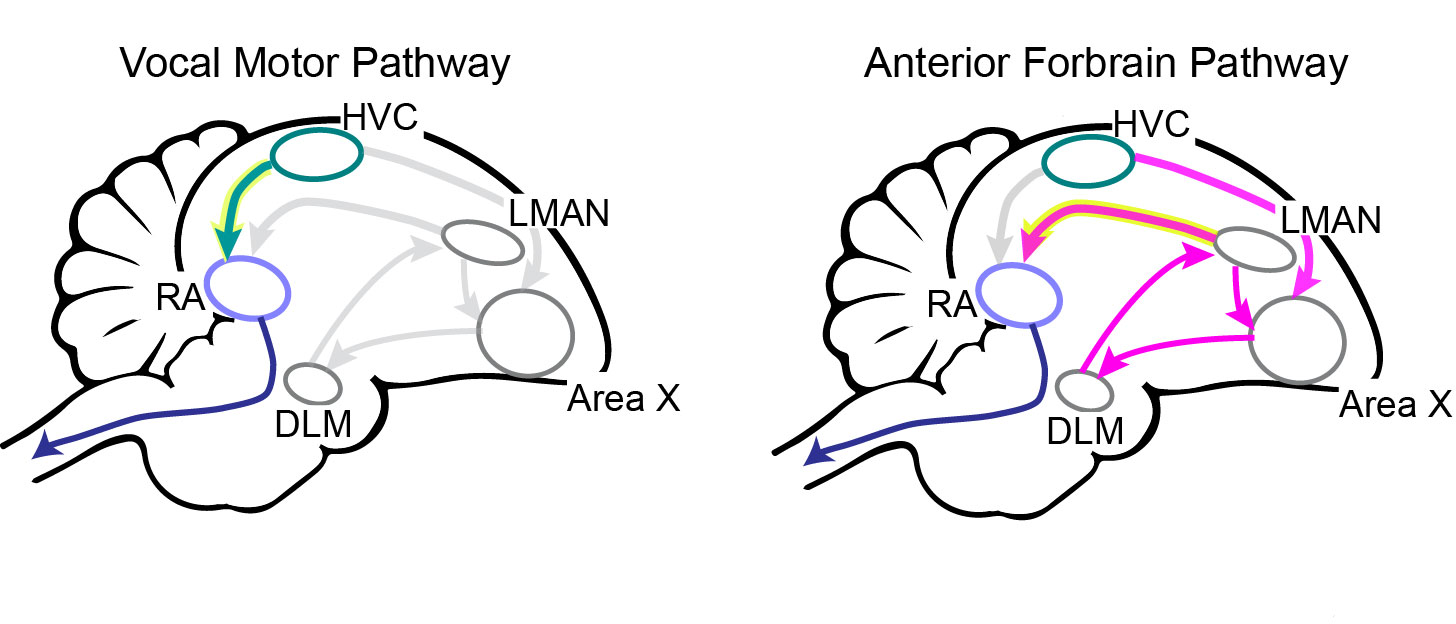
\includegraphics[width=14cm]{figure2.jpg}
    \centering
\medskip
\caption[Song circuit overview]{\footnotesize  \textbf{Song circuit overview.} \textbf{a}, \textit{Left,} Vocal Motor Pathway \textbf{(VMP)}, which acts as a simple motor hierarchy.  \textit{Right,} the Anterior Forebrain Pathway \textbf{(AFP)}, which is involved in trial-and error vocal learning.  It is important to note that both pathways include the nuclei HVC and RA.}

\label{fig:Sampling}
\end{figure}


The neural circuitry underlying the zebra finch's song is one of the best described in neuroscience. This circuit is distributed throughout the brain in small computational engines called \emph{nuclei}, that are distributed into two primary pathways: the\emph{ vocal motor pathway} (VMP) that mediates adult, stereotyped vocal performance, and the \emph{anterior forebrain pathway} (AFP) that underlies vocal exploration and learning \cite{Aronov2008-kx} \cite{Olveczky2005-mc}. Of critical interest are two nuclei. The first is the premotor nucleus,\emph{ HVC}, which is the shared origin of the VMP and the AFP. The second is the \emph{robust nucleus of the arcopallium} (RA), a critical component of the descending motor pathway where both the VMP and the AFP converge. From RA, neurons project to the hypoglossal nucleus \emph{nXII}, in the brainstem and neurons in the caudal portion of nXII directly innervate the muscles controlling the syrinx \cite{Olveczky2005-mc} \cite{Vicario1988-dl}. RA has a weak projection to the nXII and another projection to brainstem nuclei that controls breathing \cite{Sturdy2003-ed} \cite{Krutzfeldt2004-po}. Both pathways are described in some detail below. 


\subsection{Vocal Motor pathway	}

At the apex of the VMP, there is a strong non-topographic projection from HVC to RA (Foster and Bottjer, 1998). Physiological evidence suggests that HVC neurons projecting to RA (HVC$_{RA}$) provide temporal control of song through addressing disparate, discrete locations within RA. In turn, different RA neurons innervate different muscle groups in the bird's vocal organ \cite{Fee2011-en}. Supporting this, unilateral lesions of RA in the adult result in severe deficits in vocal production (Ashmore et al., 2008), whereas unilateral lesions of HVC mostly affect song sequencing \cite{Williams2004-hn}. This effect is relatively subtle compared to bilateral lesions that cause adults to revert to juvenile-like subsong \cite{Aronov2008-kx}. A one-to-many projection from HVC to RA would allow individual HVC$_{RA}$ neuron bursts to coordinate the activity of multiple muscles at a single point in time. In this way, the VMP is simply a motor control hierarchy.


\subsection{Anterior Forebrain Pathway (AFP)}

Anatomically, in the AFP, projection neurons begin in HVC, which sends axons to the striatopallidal nucleus \emph{Area X}. This area shares strong physiological similarities to the mammalian basal ganglia \cite{Goldberg2010-fm}  \cite{Fee2011-en}. Pallidal neurons in Area X project to the dorsolateral division of the medial thalamus (DLM). DLM, in turn, projects to LMAN, which sends bifurcating axon collaterals to both RA and back to Area X \cite{Nixdorf-Bergweiler1995-nj}  \cite{Vates1995-zr}. Lesions of LMAN or Area X have not been shown to have a pronounced effect on the structure or timing of adult song \cite{Olveczky2005-mc} (Scharff and Nottebohm, 1991) (Sohrabji et al., 1990). However, lesions of either DLM or LMAN in juveniles and adults result in a significant decrease in trial-to-trial song variability and song stereotypy increases \cite{Aronov2008-kx}  \cite{Fee2011-en} \cite{Kao2006-gp}  \cite{Olveczky2005-mc}. Alternatively, bilateral lesions of HVC in adult birds leads to a regression of song to a state that resembles juvenile-like babbling \cite{Aronov2008-kx} . Together, these results suggest that the AFP, specifically the LMAN $\rightarrow$ RA projections, provides a source of trial and error variability, where the evaluation of this variation could form the basis of trial and error learning. Still, the basic mechanisms of how the AFP injects noise into RA, and how beneficial noise is incorporated into the VMP, remain to be directly observed. 
 
These theories have been tested explicitly in studies where the bird must shift the pitch of a targeted syllable to avoid playback of aversive white noise \cite{Andalman2009-lj} \cite{Tumer2007-oj}. If the AFP is inactivated after multiple days of learning, the pitch will revert back to the outcome of the previous day's learning. \cite{Tumer2007-oj} This observation strongly implies that the AFP rapidly generates fluctuations to explore advantageous variations and mediates fast learning and that VMP learns new motor programs slowly, potentially over periods of sleep \cite{Andalman2009-lj}.  


\subsection{HVC physiology}

Projection neurons in HVC can be broadly classified by their downstream projection targets, including basal ganglia-projecting neurons (HVC$_{X}$) that project to the AFP and are thought to be involved in trial-and-error learning and motor projecting neurons (HVC$_{RA}$), which in turn project to brainstem respiratory and vocal nuclei that directly drive the vocal organ \cite{Krutzfeldt2004-po}. A third, much larger projection neuron type that innervates the auditory region avalanche (HVC$_{AV}$) also sparsely populates the nucleus.
Individual HVC neurons fire a brief, 10ms volley of action potentials (where firing rates can exceed 100Hz!) at the same point in a song over many repetitions \cite{McCasland1987-cf}, sparsely coding for points in time throughout the song. \cite{Hahnloser2002-nl}. HVC$_{RA}$ neurons burst at a single point in a song with < 1ms onset jitter between repetitions of the same song. HVC$_{X}$ cells appear to share the same sparse coding properties of HVC$_{RA}$ neurons, though they tend to burst more than once per motif \cite{Kozhevnikov2007-jz}. HVC$_{I}$ neurons produce dense, complex, repeating patterns. Given that the downstream neurons in RA burst at many points throughout the song \cite{Leonardo2005-up}, it has been proposed that there is a many-to-one projection from HVC$_{RA}$ neurons. This convergence would allow single HVC$_{RA}$ neurons to act as the ticks of a clock with each 'tick' triggering the recruitment of multiple muscle groups as needed throughout the song.
 
Mild cooling of HVC with a bilaterally implanted Peltier device results in linear stretching of spectral components of a song, whereas cooling of RA does not affect song timing, suggesting that the neural dynamics generated by intrinsic circuitry within HVC controls moment-to-moment timings of acoustic features in the syllables of adult song. \cite{Long2008-go}  \cite{Fee2011-vs}. Also, dense sampling of projection neurons reveals largely uniform coverage in time \cite{Picardo2016-tj} \cite{Hahnloser2002-nl}). These results have suggested that a ballistic propagation of synaptically connected premotor neurons in HVC form a synaptic chain that forms a basic clock, dictating song timing in a top-down manner. 
However, direct excitatory synapses are sparse \cite{Kornfeld2017-lq} and excitatory neuron coupling is low \cite{Mooney2005-ev}. Moreover, it is clear that inhibition plays a large role in coordinating and stabilizing these dynamics \cite{Markowitz2013-ly}.

In a closely related species, the bengalese finch, cooling HVC alters the transition probabilities between syllables, reducing the number of repetitions of long-repeated syllables and increases the randomness of syllable sequences. In addition, HVC neurons in this species that project to the basal ganglia (HVC$_{X}$) display context-dependent activity correlated to syllable repetition and transition \cite{Wang2008-ml}. Additionally, in finches, stimulation of HVC during singing can terminate, restart, or rearrange song syntax \cite{Vu1998-gz}  \cite{Wang2008-ml}. Furthermore, UVA, an upstream input to HVC, displayed activity locked to the offsets of song motifs and song bouts. Taken together, this evidence suggests that timing and probabilistic sequencing of motor action can share the same localized neural circuit within HVC and that it can be influenced by its upstream inputs. 
 
	
Previous studies of HVC have only characterized the activity of small numbers of single neurons recorded serially \cite{Hahnloser2002-nl} \cite{Kozhevnikov2007-jz} Long et al., 2010; Yu and Margoliash, 1996). Until the work described in this thesis, no group has directly observed the relationship between single cells and network activity during the production of song. Rectifying the mismatch between models describing HVC dynamics and the lack of experimental data to validate them is a critical aim of this thesis. Even now, we are still only taking the first steps toward a long journey of understanding HVC at single cell resolution, and on a network scale. For example, basic questions about network function, such as how and to what degree the stability of neuronal activity is balanced with plasticity in brain circuitry, has been largely ignored- primarily because addressing these challenges requires longitudinal measurements from the same neurons in vivo, which has been difficult to achieve using classical neurophysiological techniques. The work described in the following chapters only scratches at the surface of these mysteries. 




%%%%=========[ Extra crap ===========%%



%\bigskip

%{\it Consider the following Java-JDT plugin name in German: "`Plugin-Entwicklungsumgebung"'.}

%\bigskip

%Clearly, this is a problem, and BU librarians will complain. One way of fixing
%this issue is to enclose the offending paragraph in {\tt
%	$\backslash$begin\{sloppypar\}} and {\tt $\backslash$end\{sloppypar\}},
%resulting in the following outcome:

%\bigskip

%\begin{sloppypar}
%	{\it Consider the following Java-JDT plugin name in German:
%		"`Plugin-Entwicklungsumgebung"'.}
%\end{sloppypar}

%\bigskip

%Indeed, although the paragraph spacing becomes sloppy, at least you can hand in
%the thesis!


%LaTeX has a steep learning curve. You can use the original book by Lamport to
%learn more \cite{lamport1985:latex}, but there are many on-line resources with
%excellent instructions and examples. Just Google a LaTeX topic you would like to
%explore.

%As far as editing and compilation of LaTeX sources, if you have not found one
%yet, TexStudio seems to be quite popular.


\cleardoublepage

% -------------------------------------
% CHAPTER 2: THE BODY OF THESIS
% -------------------------------------

  \newpage
  
  \clearpage
\vspace*{\fill}
\begin{center}
\begin{minipage}{.6\textwidth}



\centering{\Large{\textbf{Part I} \\
Engineering tools for long term neural recording in small animals.}}

\end{minipage}
\end{center}
\vfill % equivalent to \vspace{\fill}
\clearpage



  \newpage
  


\chapter{A carbon-fiber electrode array for long-term neural recording}
\label{chapter:body}
\thispagestyle{myheadings}

% set this to the location of the figures for this chapter. it may
% also want to be ../Figures/2_Body/ or something. make sure that
% it has a trailing directory separator (i.e., '/')!
\graphicspath{{2_Body/Figures/}}

This chapter is a reproduction of previously published work \cite{Guitchounts:2013bs}, and contains critical contributions from \emph{Dr. Jeffery Markowitz}, as well as \emph{Gregory Guitchounts}, who are equal co-authors on this manuscript. 

\section{Introduction}


A powerful approach to the study of learning involves tracking neural firing patterns across time. Optical methods for stable recording are developing rapidly (Harvey et al., 2012) but the temporal resolution of electrical recordings remains unsurpassed, and chronically implanted microelectrodes are central to scientific studies of neural circuit function in behaving animals, and central to the development of intracranial brain-machine interfaces in humans (Donoghue, 2008). In primate motor cortex, relatively large neurons can be tracked for weeks (Dickey et al., 2009; Fraser and Schwartz, 2012; Tolias et al., 2007) using commercially available electrode arrays. This has enabled researchers to study the stability of motor tuning (Chestek et al., 2007; Rokni et al., 2007) and the process of memory formation (Kentros et al., 2004; Thompson and Best, 1990); and it has provided the basis for brain machine interface technologies (Koralek et al., 2012).
Over time, chronically implanted electrodes are severely limited by a tissue reaction that eventually encapsulates the electrode, killing neurons in the vicinity of the electrode. The limitations of this tissue response are particularly acute if the goal is recording from densely packed neurons in small brains. For a silicone array whose cross- section is 15x200 $\mu$m, histological markers of gliosis and neuron death reveal tissue damage extending up to 300 $\mu$m or more from the implant (Biran et al., 2005). This length-scale of tissue damage does not prohibit long term recording from pyramidal neurons in primate cortex whose large polarized dendrites and large somas (up to 100 $\mu$m) produce a strong signal for extracellular recording. However, the length scale of tissue damage becomes prohibitive when recording from many cell types in smaller organisms. For example, in the songbird nucleus HVC (used here as a proper name), somas are only 8-15 $\mu$m in diameter (Mooney and Prather, 2005) and closely-packed in clusters making soma-soma contact (Scott et al., 2012). Dendrites in HVC are also compact (40-100 $\mu$m radius), and spherical in shape rather than polarized (Katz and Gurney, 1981; Lewicki, 1996; Mooney and Prather, 2005). To isolate the weak signal generated from these cells, electrodes with small recording surfaces are advanced with motorized microdrives, allowing $\mu$m-scale control over electrode positioning. The absence of any report of single neuron isolation in HVC with a fixed chronic electrode implant underscores the difficulty of recording small cells with an implant whose damage length scale is large relative to the target neurons. Examples of multi-day recordings in mouse hippocampus can be found (Kentros et al., 2004; Koralek et al., 2012) that employ movable tetrode microwires, but recording methods that make this process more efficient are needed. Ultimately, to facilitate long term recordings from densely packed neurons in small animals, and to improve the longevity of human and primate neural interfaces, electrode designs are needed that reduce chronic tissue damage. The cross-section of implanted electrodes must be minimized to reduce chronic disruption of the blood brain barrier (Biran et al., 2005; Polikov et al., 2005). Orthogonal pressures are driving an increase in the number of recording sites per implant, but increasing the density of recording sites may be counter-productive if the implant size also increases. 

Recently proposed carbon fiber ultramicroelectrodes promise to reduce damage
upon implantation, and may partially evade immune rejection (Kozai et al., 2012). Glass insulated carbon fibers have been used for cyclic voltammetry and extracellular recording for some time (Armstrong-James and Millar, 1979; Garris et al., 1994), but the essential advance of the proposed microthread electrode involves doing away with the large-diameter glass insulation in favor of a thin (1 $\mu$m) layer of parylene deposited over a small (3-7$\mu$m) diameter carbon fiber. This also serves to dramatically reduce the stiffness of the implant, another factor hypothesized to contribute to tissue damage (Subbaroyan et al., 2005). The small profile over the full length of the electrode, in principle, could provide for minimal chronic tissue damage and neuron death. The small scale of the proposed carbon microthread electrode makes implantation challenging. Practical methods for building and implanting high channel-count carbon fiber electrodes remain undefined. The present study describes one such design.

The 16 channel carbon fiber array described here has a final cross-section of approximately 26  $\mu$m, on par with single micro-wires in commercial microwire arrays (30-50$\mu$m wires in all Tucker Davis microwire arrays, for example.) The principle innovations of this work arise from carbon fiber manipulations using the elements of fire, air and water: burning partially submerged carbon fibers leads to a consistent electrode tip preparation. Drawing carbon fibers through an air-water interface leads to surface-tension driven bundling of the fibers, resulting in an implantable array. To test the design, we examined the neural representation of song execution in zebra finches- a uniquely tractable test-bed for assessing chronic electrode stability. Zebra finch song is a stereotyped natural behavior produced by a distinctive learned pattern of neural activity. As the bird sings, each of three cell types in pre-motor nucleus HVC interneurons, basal ganglia-projecting neurons, and motor output neurons discharge in a stereotyped, characteristic pattern with minimal spike-time jitter ($<$1 ms for motor output neurons) between renditions of the same song (Hahnloser et al., 2002; Kozhevnikov and Fee, 2007).

The various cell types in HVC are small (8-15  $\mu$m), and synchronous elevated firing rates of interneurons during song make isolation of single units challenging. Current approaches to recording the three cell types in HVC require the use of high impedance electrodes positioned close to individual cells using a motorized microdrive (Fee and Leonardo, 2001). Neurons isolated in this manner in HVC are typically not recorded for a time-scale longer than tens of minutes. Using fixed implants of the carbon fiber arrays described here, we recorded unambiguous single units in HVC over timescales of 4-12 hours, and sorted multi-unit clusters over time-scales of months. We find that the precise temporal patterns recorded in HVC are stable over the time-scales of our recordings. This feature provides a means of validating signal stability independently of spike waveforms, providing a useful test-bed to assess chronic recording methods.


\section{Results}
\subsection{Fire Sharpening}

The underwater firing process exposed 89 $\pm 17$  (SD) $\mu$m of insulation as measured by widefield and confocal microscopy (n = 34 tips), leaving sharpened, uniform tips (see SEM images in Figure 2$\cdot$1c and fluorescent parylene images in Figure 2$\cdot$2). The torching process produced tips with an average impedance of 1.26 M$\Omega$ (n = 210 tips) (Figure 2$\cdot$3a). Impedances measured in vivo after implanting showed a wide range of values in the weeks following implant (Figure 2$\cdot$3b).

\begin{figure}[!htb]
 %\begin{minipage}[t]{0.49\linewidth}\centering
    \includegraphics[width=8cm]{chapter2/figure1.png}
    \centering
\medskip
\caption[Array assembly.]{\footnotesize  \textbf{Array assembly.} \textbf{a}, \textit{Left,} Diagram of the 3D-printed plastic block with wells for 16 carbon fibers. Fibers are threaded through the wells on the top of the block and exit through the hole on the bottom. \textit{Middle}, To expose the connector-side ends of the fibers from parylene, the fibers are heated by passing them through a gas/oxygen torch. \textit{Right}, The wells are then filled with conductive silver paint to make electric contact with an Omnetics connector, which slides into the plastic block wells. \textbf{b}, Fire-sharpening of electrode tips. \textit{Left}, the assembled array is lowered into a water bath with the tips of the carbon fibers protruding above the surface of the water. \textit{Bottom}, SEM image of a blunt cut carbon fiber electrode, with insulation frayed near the tip. \textit{Middle}, A gas/oxygen torch is passed over the surface of the water, burning the carbon and the insulating parylene down to the water surface. \textit{Bottom}, After passing the torch over the exposed tips, the carbon fiber tapers to a sharp point. \textit{Right}, The array is then taken out of the water, with the tips pointing down; surface tension acts to bring the carbon fibers into a single tight bundle. \textbf{c}, The assembled array. The 16-electrode bundle is approximately 26 $\mu$m in diameter (upper right). The immersion tip burning process exposes approximately 89 $\mu$m of carbon (lower right).}
\label{fig:Sampling}
\end{figure}


\begin{figure}[!htb]
 %\begin{minipage}[t]{0.49\linewidth}\centering
    \includegraphics[width=12cm]{chapter2/figure2.png}
    \centering
\medskip
\caption[Wide-field imaging of a coated carbon fiber.]{\footnotesize  \textbf{Wide-field imaging of a coated carbon fiber.} \textbf{a}, \textit{Left}, wide-field image of a carbon fiber coated in fluorescent Parylene-C, after it had been fire-sharpened. \textit{Middle}, UV filter image for the same fiber. \textit{Right}, Merged images of the wide-field and fluorescence view shows that the fire sharpening method exposes an average of 89 $\pm 17$ $\mu$m. \textbf{b}, Another example fiber.}
\label{fig:Sampling}
\end{figure}

\subsection{Acute recordings}

To initially assess the viability of carbon fiber electrode arrays for recording at various depths we recorded extracellular signal acutely in anesthetized or awake head-fixed birds (n=4 cells from 4 birds). Figure 2$\cdot$4 shows average waveforms from well-isolated neurons and spike trains recorded in auditory area Field L in awake head-fixed birds with an SNR of 9.18 and 3.00 (Figure 2$\cdot$4a and 2$\cdot$4d, respectively); in premotor nucleus HVC in an anesthetized bird with an SNR of 21.64 (Figure 2$\cdot$4b) and in basal ganglia nucleus Area X in an anesthetized bird with an SNR of 3.50 (Figure 2$\cdot$4c). Carbon fiber arrays were thus able to measure signals from a range of cell types across a variety of brain regions, including a recording zone 3.0 mm deep (Area X).

\begin{figure}[!htb]
 %\begin{minipage}[t]{0.49\linewidth}\centering
    \includegraphics[width=9cm]{chapter2/figure3.png}
    \centering
\medskip
\caption[Electrode impedances.]{\footnotesize  \textbf{Electrode impedances.} \textbf{a}, Histogram of the fire-sharpened pre-implant electrode impedance (n = 210 fibers; median = 1.0M$\Omega$). \textbf{b}, Impedance of fibers in 7 implanted arrays measured at various time points after implanting. Colors indicate fibers grouping into arrays. The pre-implant impedances (in saline) in corresponding colors are shown at Day 0.}
\label{fig:Sampling}
\end{figure}

\begin{figure}[!htb]
 %\begin{minipage}[t]{0.49\linewidth}\centering
    \includegraphics[width=9cm]{chapter2/figure4.png}
    \centering
\medskip
\caption[Average waveforms of isolated single units recorded acutely with 16 channel carbon fiber arrays.]{\footnotesize  \textbf{Average waveforms of isolated single units recorded acutely with 16 channel carbon fiber arrays.} \textbf{a}, A unit recorded in auditory area Field L in an awake head-fixed bird (SNR=9.18). \textbf{b}, A unit from the pre-motor nucleus HVC in an anesthetized bird (SNR=21.64). \textbf{c}, An isolated unit found in the basal ganglia of an anesthetized bird (SNR=3.50). \textbf{d}, A unit recorded in Field L of an awake, head-fixed bird (SNR=3). Insets show corresponding spike trains . Inset scale bars: (A) 200 $\mu$V, 50 s; (B) 400 $\mu$V, 100 s; (C) 100 $\mu$V, 1 s; (D) 100 $\mu$V, 5 s. Pink indicates standard deviation.}
\label{fig:Sampling}
\end{figure}

\subsection{Single-unit recordings in freely behaving birds}

Our primary goal was to develop an electrode capable of tracking single units and small multi-unit clusters over extended periods of time. Thus, to assess the reliability and longevity of single cell signal, we implanted 16 channel carbon fiber arrays into the premotor nucleus HVC (n=10 birds), an area that produces precise neural firing patterns that ultimately drive muscular sequences to produce song (Long et al., 2010).

Spikes were aligned to all renditions of a given vocal element for a single day and displayed as a raster plot (Figure 2$\cdot$5). Figure 2$\cdot$7 shows one such raster from a putative HVC interneuron (classified as single-unit by the standard criterion, see Section 2.3.5) recorded over a period of 15 days. Average waveforms and ISIHs from the 1st, 7th and 14th days are consistent throughout the period (Figure 2$\cdot$6). The average firing patterns are also stable over these time-scales.

\begin{figure}[!htb]
 %\begin{minipage}[t]{0.49\linewidth}\centering
    \includegraphics[width=12cm]{chapter2/figure5.png}
    \centering
\medskip
\caption[Single-unit recording in a singing bird.]{\footnotesize  \textbf{Single-unit recording in a singing bird.} Example of a putative interneuron recorded in the pre-motor nucleus HVC aligned to song. \textit{Top}, the time-frequency histogram of aligned renditions of the same song motif. \textit{Middle} and \textit{Bottom}, spike raster from a single unit aligned to song and a raw trace from the same channel.}
\label{fig:Sampling}
\end{figure}

Additionally, in some cells we found distinctive waveforms and discharge patterns characteristic of principal neurons; that is, sparse high-frequency bursting aligned to a single point in the birds song (Figure 2$\cdot$8). The cell recorded for this figure met the standard criterion for single unit isolation. Prior recordings of this neuron type have required high impedance electrodes mounted on motorized microdrives that allow for fine positioning of the electrode in the vicinity of the neuron (Hahnloser et al., 2002). This is the first report of HVC projection neuron recordings from immobile chronic implants. The yield and longevity of all recorded neuron types are reported below.

\begin{figure}[!htb]
 %\begin{minipage}[t]{0.49\linewidth}\centering
    \includegraphics[width=11cm]{chapter2/figure6.png}
    \centering
\medskip
\caption[Clusters for the chronic signal]{\footnotesize  \textbf{Clusters for the chronic signal shown in previous figure.} \textit{Top row}, overlaid spike waveforms. \textit{Middle row}, spike waveform histograms. \textit{Bottom row}, spike ISIHs. The SNR changed from 2.39 on Day 1 of recording (left column) to 3.29 on Day 7 (middle column) and 2.09 on Day 14 (right column).}
\label{fig:Sampling}
\end{figure}


\begin{figure}[!htb]
 %\begin{minipage}[t]{0.49\linewidth}\centering
    \includegraphics[width=11cm]{chapter2/figure7.png}
    \centering
\medskip
\caption[Chronic recording stability in the singing bird.]{\footnotesize  \textbf{Chronic recording stability in the singing bird.} \textit{Top}, A putative HVC interneuron (single unit by the standard criterion) in bird recorded over 15 days. \textit{Bottom}, raw traces from the same channel on days 1, 7 and 14. Signal fading (as on day 14) indicates periods of partial loss of cell isolation.}
\label{fig:Sampling}
\end{figure}


On two occasions, a portion of the sharpened tip of an electrode apparently entered a cell, yielding intracellular-like traces that were stably held for 12 hours in one case and 36 hours in the next (Figure 2$\cdot$9). The intracellular-like cells recorded in area X and HVC were characterized by high amplitude spikes and positive subthreshold voltage ramps prior to spikes or bursts and stereotyped hyperpolarizing potentials following the burst in the area X cell. In these rare recordings a portion of the uninsulated (80 $\mu$m) tip must have remained outside the cell (Angle et al., 2012).

\subsection{Simultaneously recorded traces}

Of particular interest in multi-electrode recordings is not only the longevity of single- unit signal, but the ability to record multiple signals at once. In chronic implants of carbon fiber arrays, high quality multi-unit signal was often present on the majority of electrode contacts, though multiple rigorous single units were not recorded simulta- neously on any implant. With the small diameter and proximity of electrodes, individual neurons were occasionally visible on multiple channels simultaneously. Features of correlated signal across channels (i.e. tetrode effect) are commonly necessary to isolate densely packed neurons, but these features were not used here. However, we have observed  examples of channels with common signal on two channels from birds implanted with 16 channel arrays. This examples illustrate the potential of improving single unit isolation based on multi-electrode features in future carbon fiber electrode designs.



\subsection{Yield and single unit stability}

Single units defined by standard criteria were defined as containing (1) adequate SNR ($>$ 1.1) and (2) a minimal fraction of ISIs shorter than a refractory period of 1 ms ($<$ 5). After discarding clustered units that did not meet these criteria, we recorded an average of 5.3 neurons per bird as defined by the standard criterion (n=6) that ranged from as few as 2 neurons to as many as 8. This count includes both putative interneurons and projection neurons, classified according to their firing patterns.

\begin{figure}[!htb]
 %\begin{minipage}[t]{0.49\linewidth}\centering
    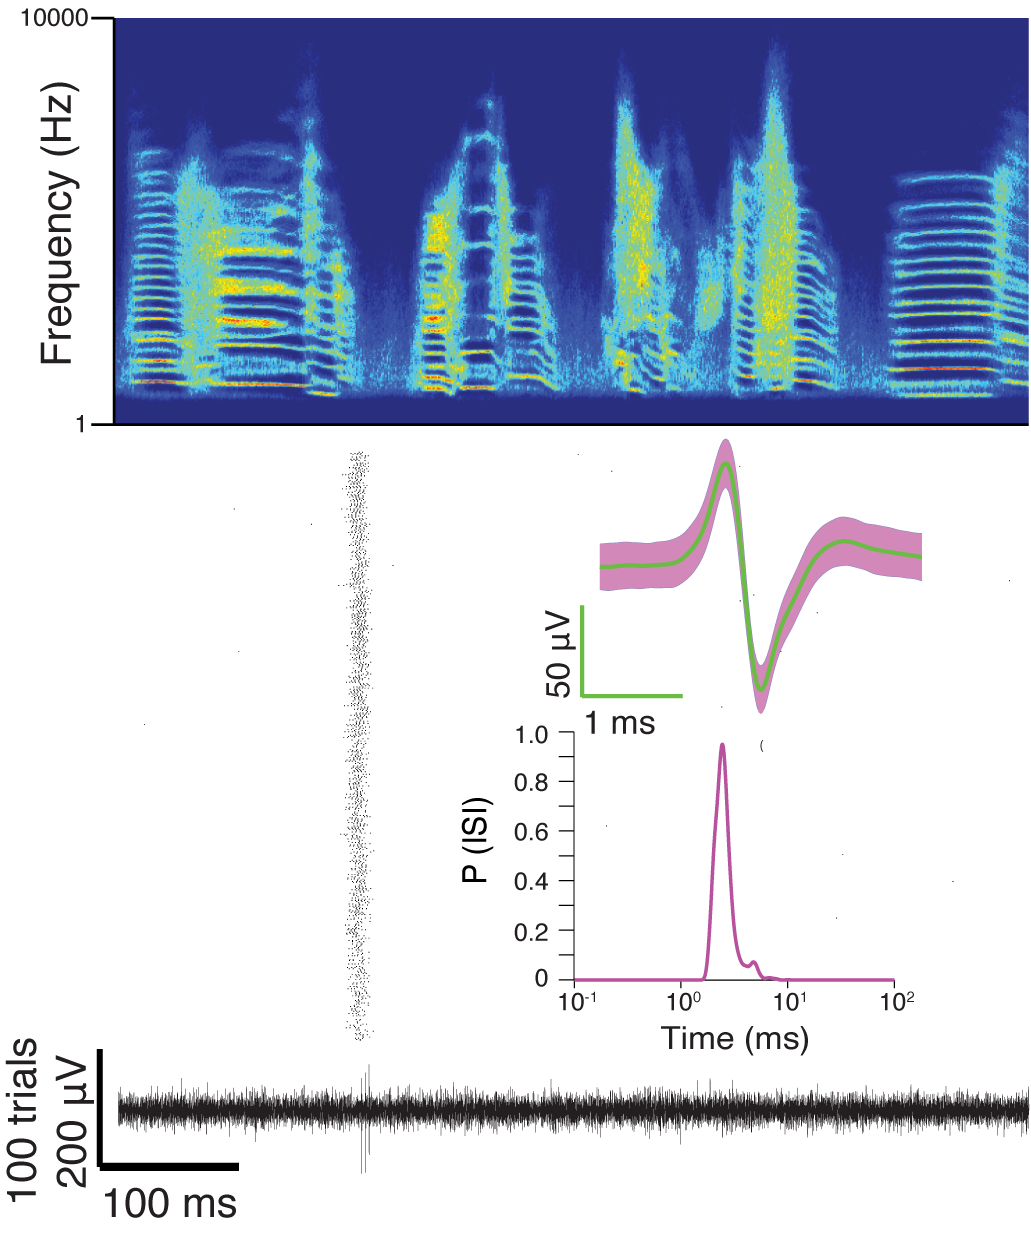
\includegraphics[width=9cm]{chapter2/figure9.png}
    \centering
\medskip
\caption[A principal cell recorded in HVC.]{\footnotesize  \textbf{A principal cell recorded in HVC.} \textit{Top}, Song-aligned spike raster of a putative RA-projecting neuron. \textit{Bottom}, The raw voltage trace from rendition 199 out of 500 song renditions recorded across 1 hour and 26 minutes. Insets show the average waveform with SD and ISI distribution.}
\label{fig:Sampling}
\end{figure}

Four rigorous single units (n=3 interneurons and n=1 projection neuron) (SNR$>$ 2.8
and 0\% ISI violations) were found in a set of n=4 implants. Finally, 16 projection neurons that did not meet the rigorous single unit criteria were recorded in at total of n=10 implants (SNR$<$ 2.8, though for this population all cells had 0\% ISI violations except two, which had 0.3\%). These cells produce a single burst one or two stereotyped times in the song, and single unit isolation could be confirmed in spite of the low SNR values. For this population of cells, we computed the fraction of contaminating spikes (spikes occurring within 100 ms of the burst, but outside a 10 ms window around the average burst time). The fraction of contaminating spikes ranged from F=0.425 in the most marginal case to F=0.008 in the best case, with an average of 0.128 $\pm$ .135
(SD). Examples of these raster plots are illustrated in Figure 2$\cdot$8.

\begin{figure}[!htb]
 %\begin{minipage}[t]{0.49\linewidth}\centering
    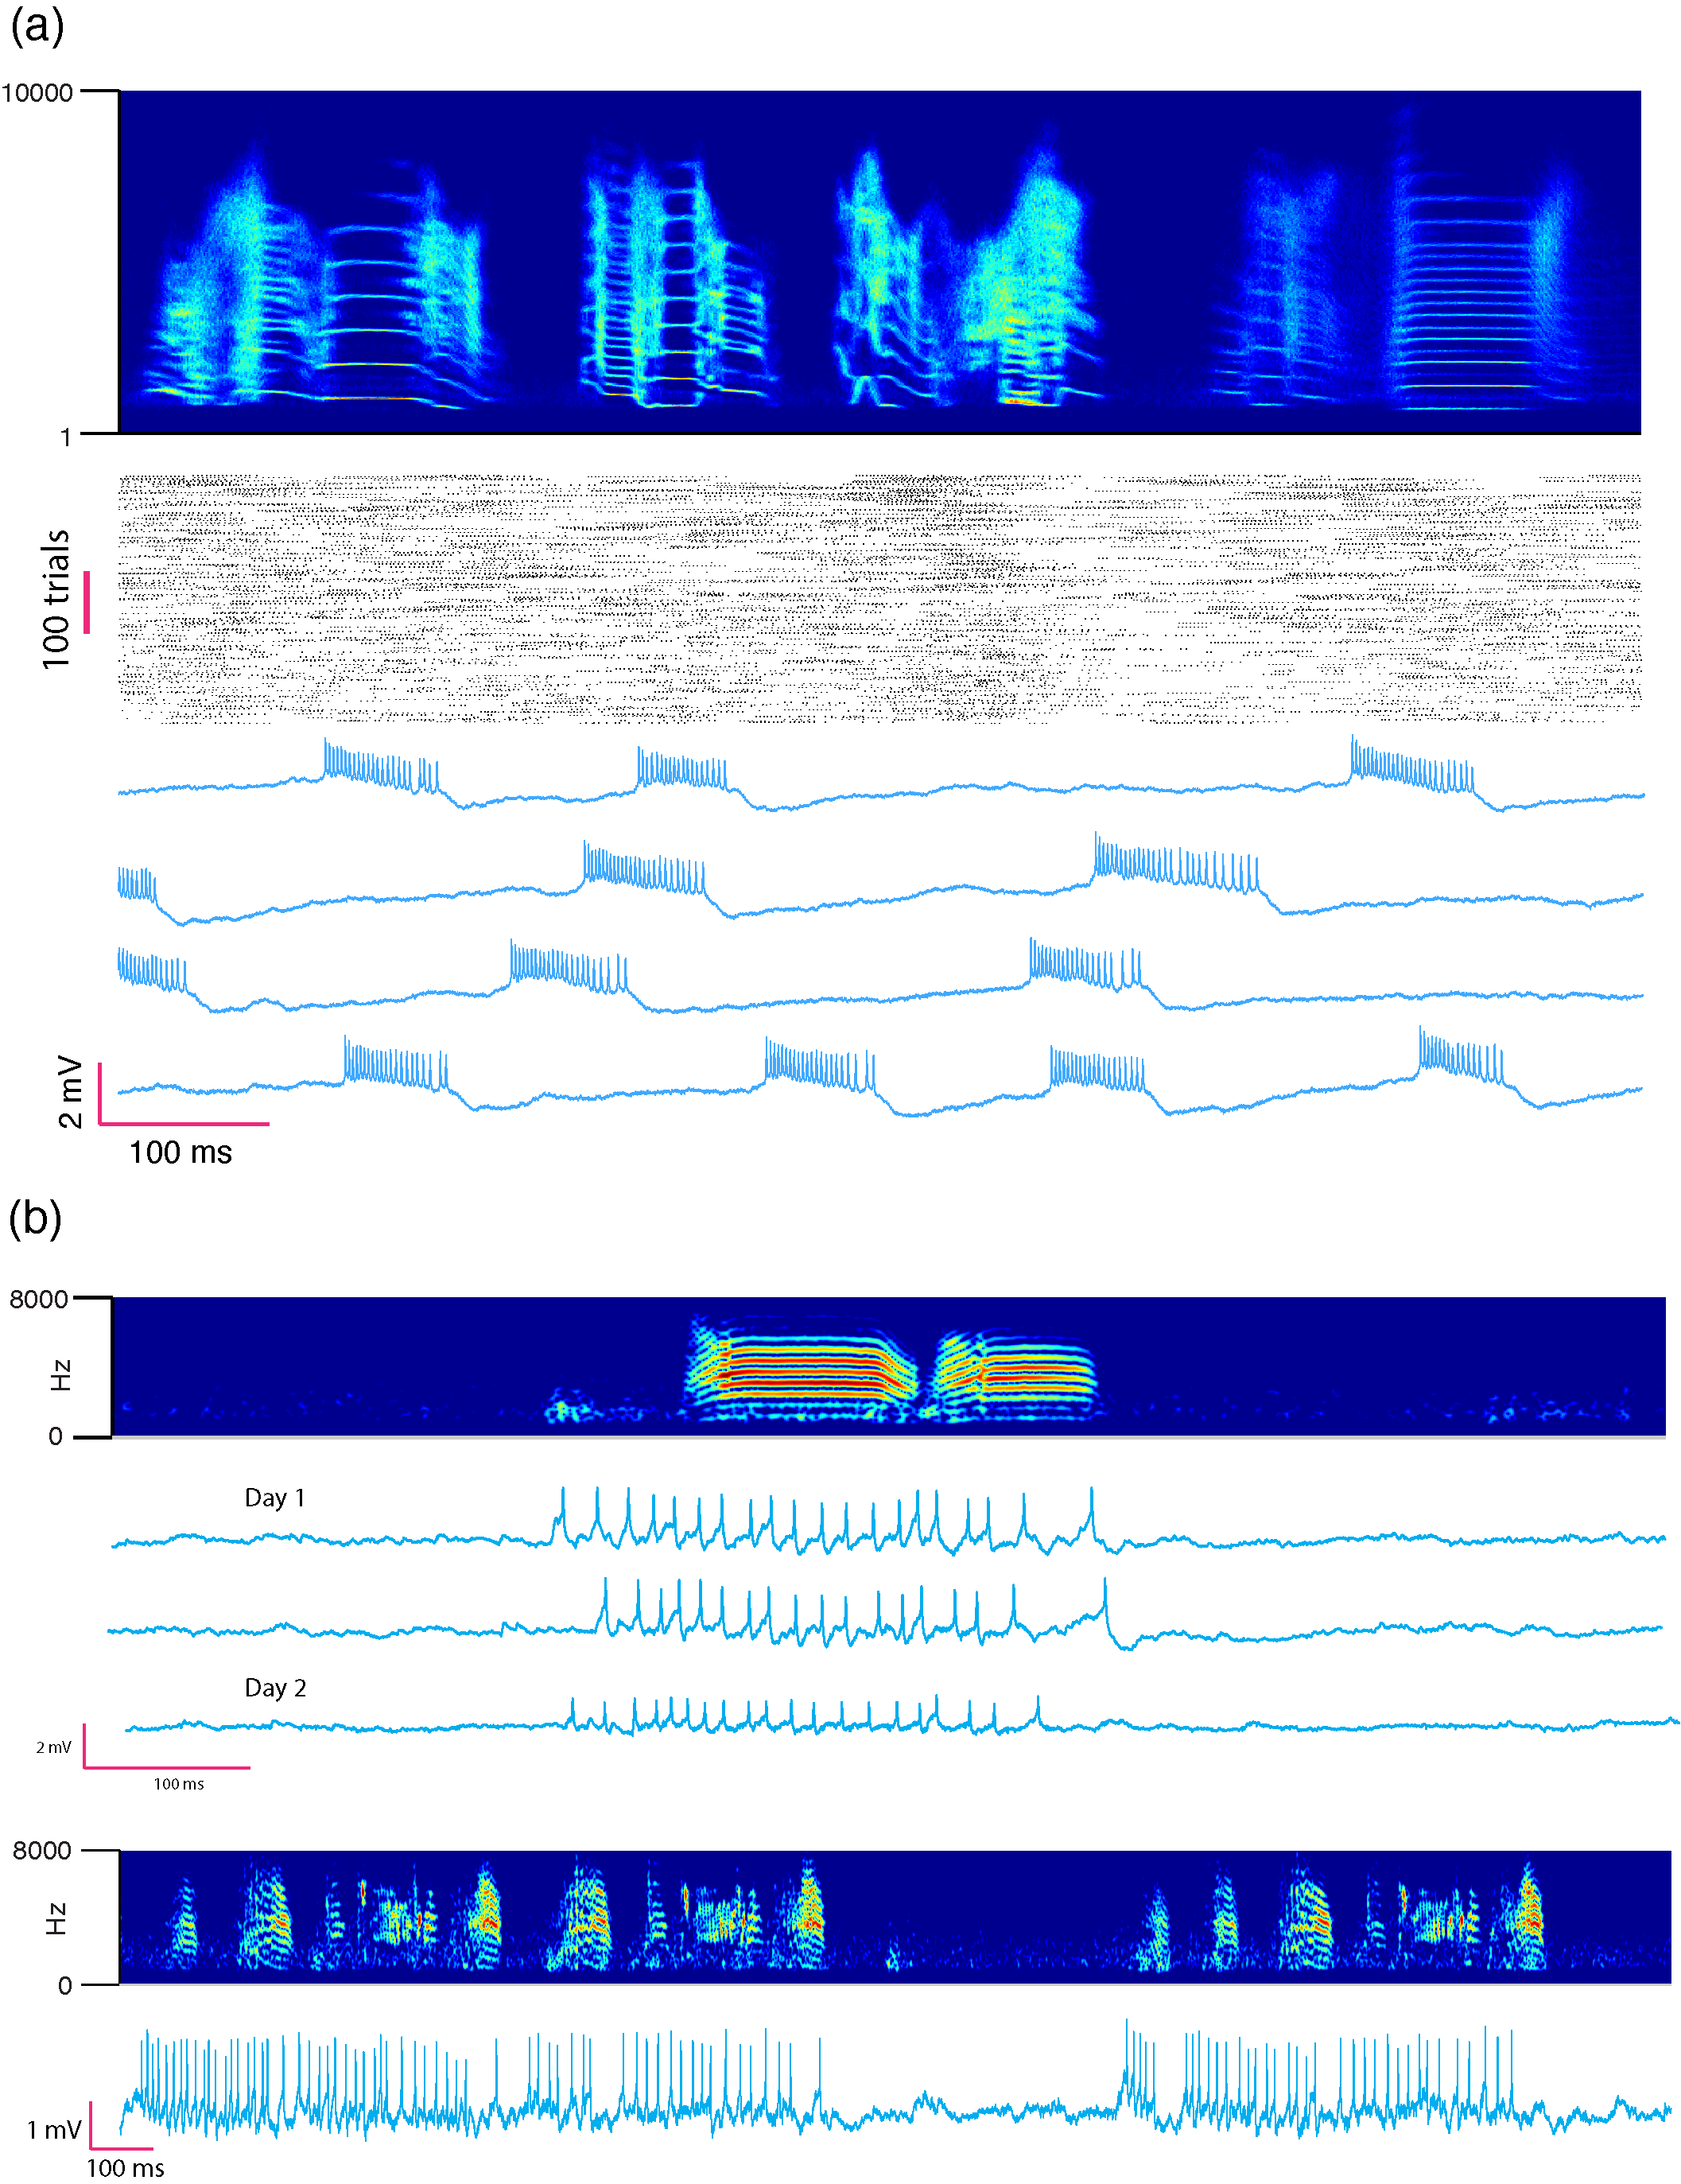
\includegraphics[width=10cm]{chapter2/figure11.png}
    \centering
\medskip
\caption[Intracellular-like traces in singing birds with carbon fibers. ]{\footnotesize  \textbf{Intracellular-like traces in singing birds with carbon fibers.} \textbf{a}, a bursting cell with high amplitude positive peaks recorded from a bird implanted in Area X. \textit{Top}, sonogram of the song; \textit{Middle}, spike raster; \textit{bottom}, low-pass filtered traces showing prominent LFP modulation during spiking. \textbf{b}, A similar cell recorded from a bird implanted in HVC. Unfiltered traces during a call, across two days (top); and during singing (bottom).
}
\label{fig:Sampling}
\end{figure}


To assess the stability of isolated units, we followed previously described methodols (Dickey et al., 2009; Fraser and Schwartz, 2012). From one day to the next, a stable waveform indicated continuity of recording from a single neuron. However, considering the population of all neurons recorded, waveform shapes were not unique, nor were ISIHs. One solution is to increase the dimensionality of the waveform shape by considering projections of the waveform on additional channels. However, in HVC of adult songbirds, a more powerful approach is possible based on the unique spike patterns produced by different neurons in HVC (Hahnloser et al., 2002; Kozhevnikov and Fee, 2007). For each neuron observed here, spike timing patterns were unique and stable across time. This is true both for clusters consisting of small numbers of cells, single interneurons (Figure 2$\cdot$10), and projection neurons (Figure 2$\cdot$8).

\begin{figure}[!htb]
 %\begin{minipage}[t]{0.49\linewidth}\centering
    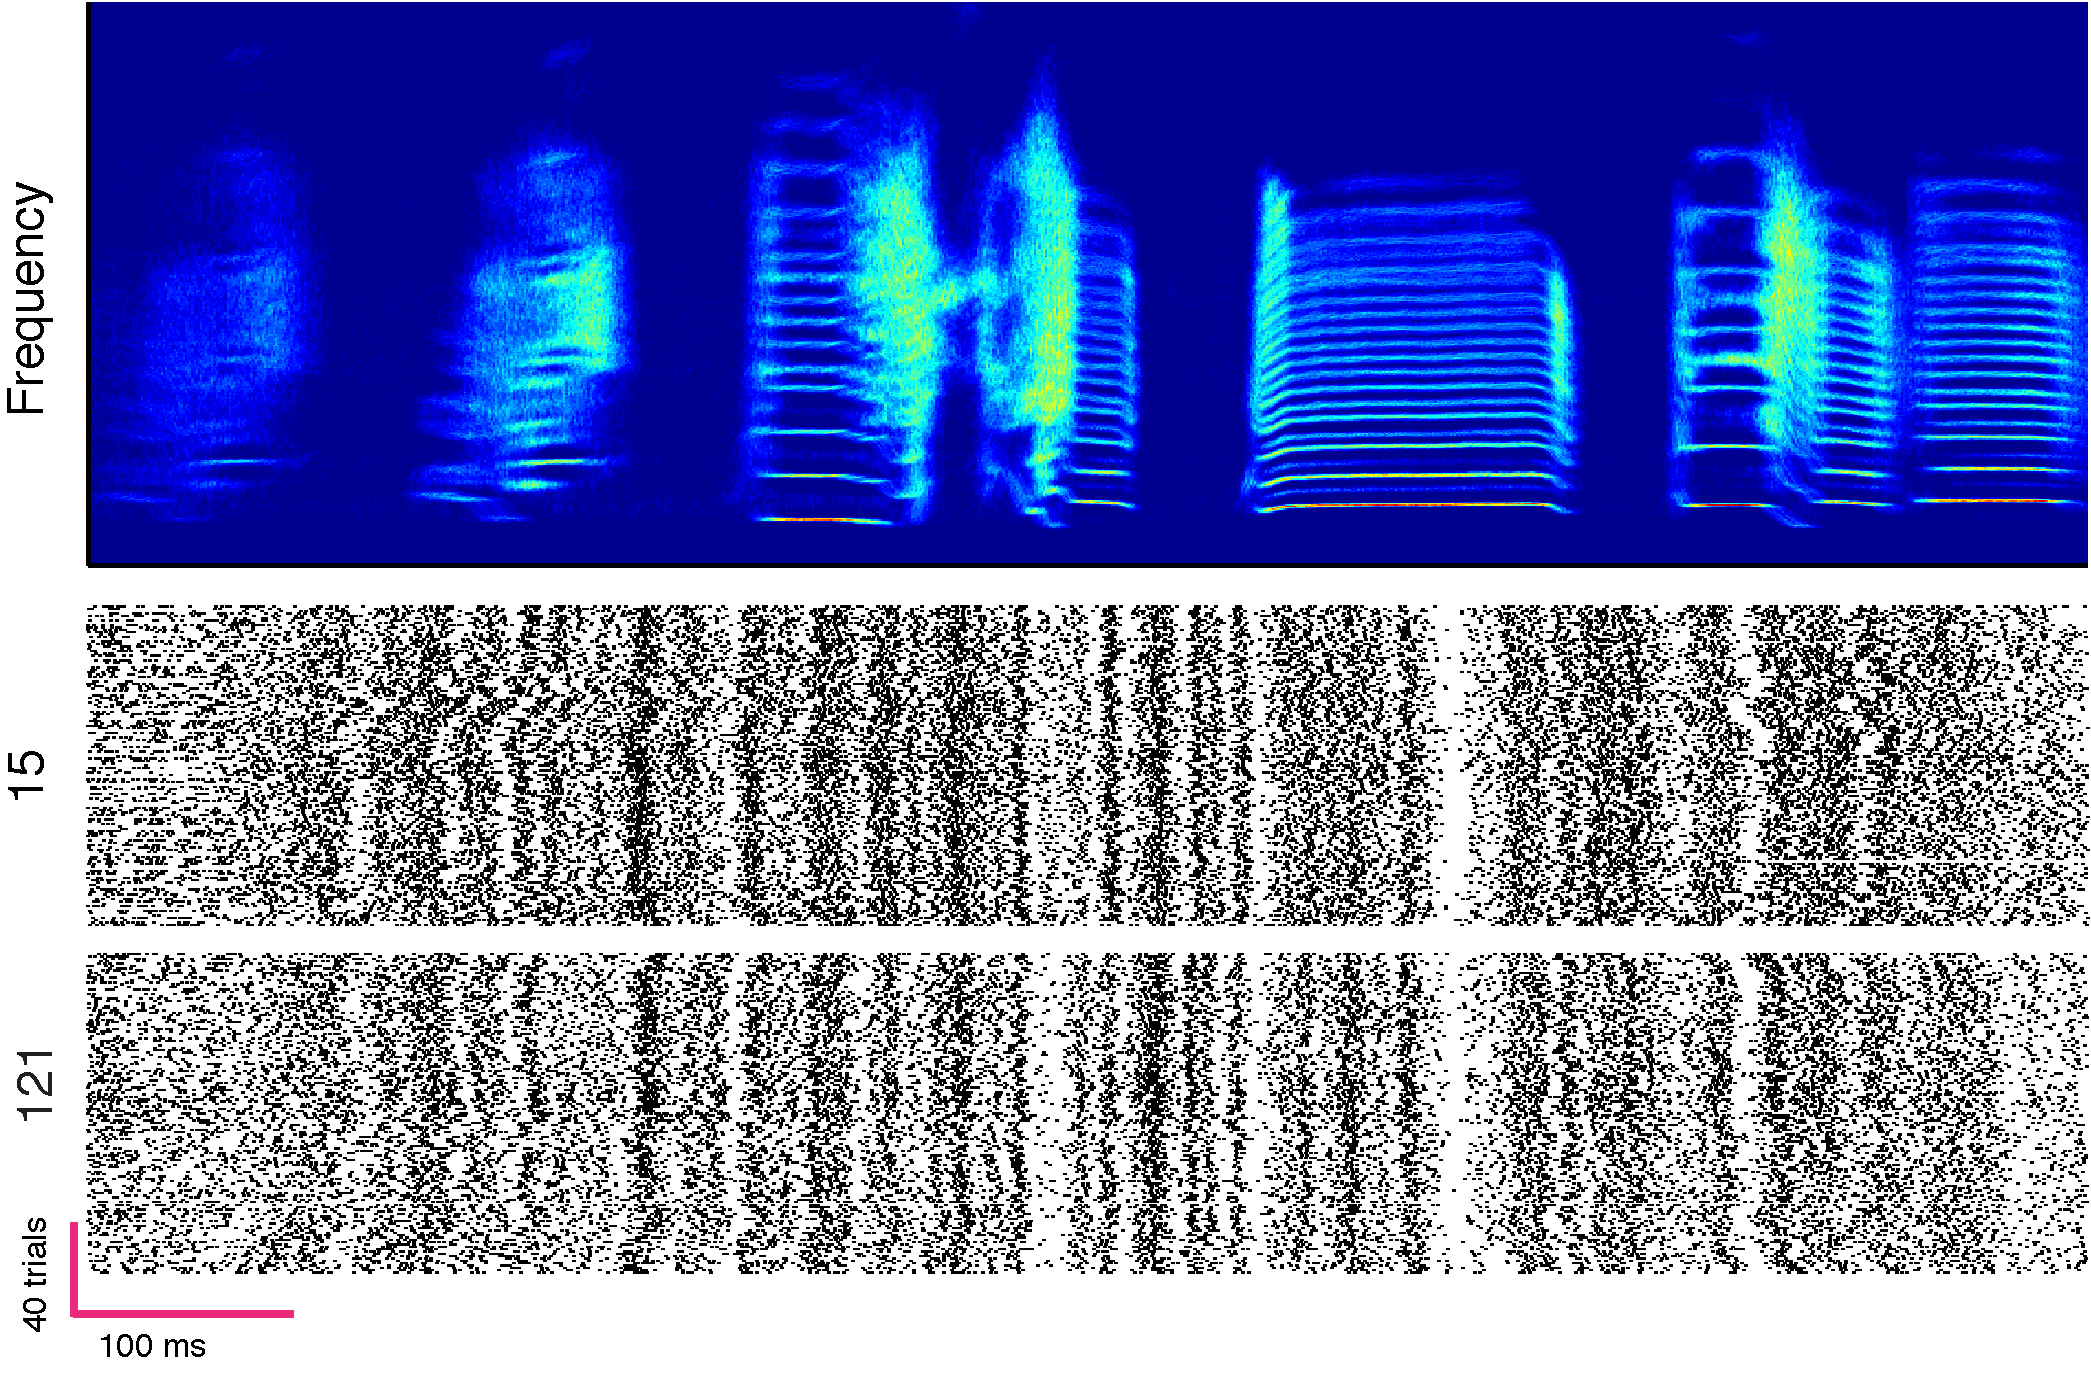
\includegraphics[width=11cm]{chapter2/figure13.png}
    \centering
\medskip
\caption[An HVC interneuron recorded on sessions 107 days apart.]{\footnotesize  \textbf{An HVC interneuron recorded on sessions 107 days apart.} Analysis on waveform shape, ISI distribution and firing pattern classifies the recordings as the same sorted cell, based on the standard criterion. Days post implant are shown on the left of each raster.
}
\label{fig:Sampling}
\end{figure}


Of the 27 neurons that passed the standard SNR and ISIH quality criteria (n=6 implants), we analyzed the 18 standard quality cells that were stable for more than one day (for the other 9, no suitable clusters on the same electrode channel were found after the first recording session). Of this set of 18, the cluster quality varied, with 5/18 having $<$ 1\% ISI violations and the rest $<$ 5\%.  Of this total, 11/18 were stable for one week, 6/18 for two weeks, and 4/18 for 30 days. Projection neurons were not recorded for more than 2 days.

For the rigorous single units (n=4) we analyzed all putative cell types. The longevity of each single unit recording is shown for each of 4 neurons, which ranges from 4 to 12 hours. (Outside of this time-scale, the cells fell below the threshold for rigorous single units, though they were still isolatable based on standard criteria that allowed for some error.)

\begin{figure}[!htb]
 %\begin{minipage}[t]{0.49\linewidth}\centering
    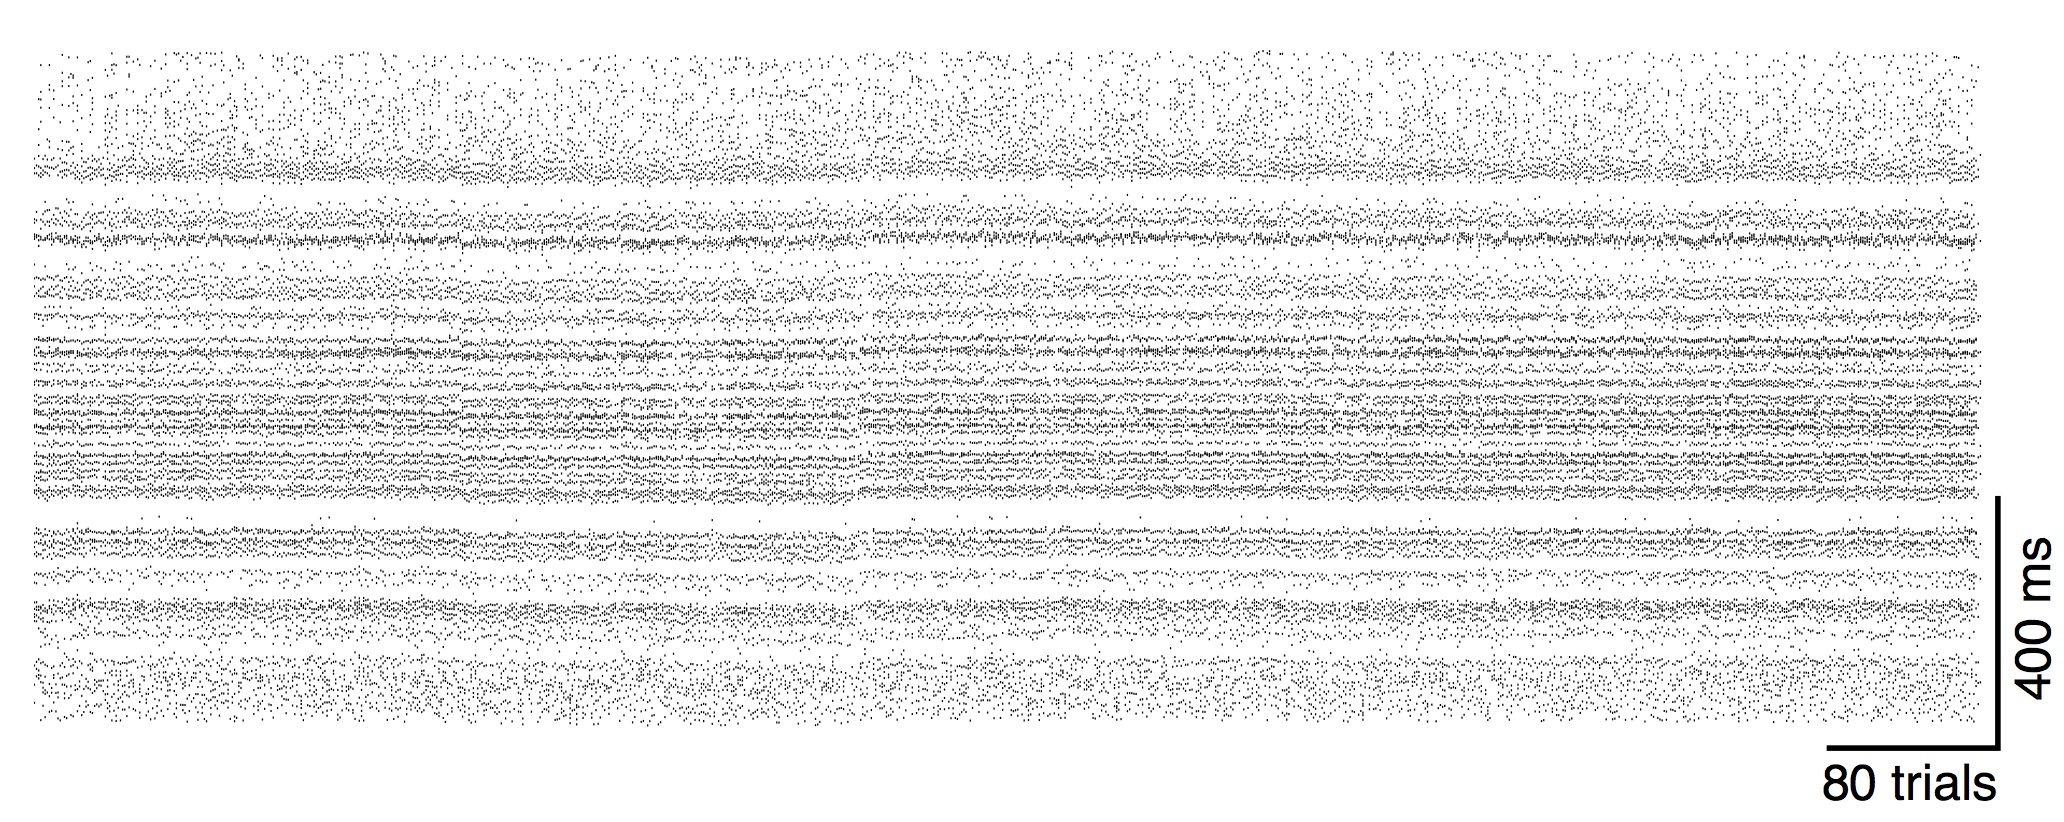
\includegraphics[width=15cm]{chapter2/figure14.png}
    \centering
\medskip
\caption[Example interneuron raster]{\footnotesize   \textbf{Spike raster for example neuron from Figure 2$\cdot$10.} All trials included in the analysis for the bottom example from Figure 2$\cdot$10 are shown in order from left to right.}

\label{fig:Sampling}
\end{figure}


\section{Methods}
\subsection{Carbon microthread arrays}


4.5-$\mu$m diameter carbon fiber threads (Goodfellow USA, Grade UMS2526) form the basis of the array. (Youngs modulus of 380 GPa compared to tungstens 400 GPa: volume resistivity 1000 $\mu\Omega$cm compared with 5.4 $\mu\Omega$cm for tungsten.)
 Epoxy sizing was removed by heating fibers at 400$^{\circ}$C for 6 hours (Lin et al., 1998) using a Paragon SC2 kiln (Paragon). A 1 $\mu$m layer of Parylene-C (di-chloro-di-p-xylylene) (Kisco) was then deposited using an SCS Labcoter 2 (PDS-2010, Specialty Coating Systems) using 2.3g of parylene and factory settings as follows: Furnace, 690$^{\circ}$C; Chamber Gauge, 135$^{\circ}$C; Vaporizer, 175$^{\circ}$C; and Vacuum at 15 vacuum units above base pressure. The integrity of the coating was verified through bubble testing initially, and defects were never found. Fourteen coated fibers and 1 coated or uncoated fiber (for the reference) were threaded through a custom plastic block designed in SolidWorks
(Dassault Systems) and 3-D printed using stereolithography (Realize Inc) (one channel out of the possible 16 was used for the microphone trace and one was shorted with the reference, making a total of 14 electrophysiology channels) (Figure 2$\cdot$1a, left). The block contains 16 wells (18x27 mils) that funnel the carbon fibers through a small aperture (12 mils in diameter) (block design files are available upon request). At this stage the carbon fibers exiting the aperture are splayed. On the top side, the block was cut to fit the straight tails of an Omnetics connector (A79038-001, Omnetics). Fibers at the mating end of the carbon were briefly passed through a gas/oxygen torch to remove insulation for making electrical contact (Smith Equipment) (Figure 2$\cdot$1a, middle). The fibers were then connected to an Omnetics connector using conductive silver paint (Silver Print part no. 842-20G, MG Chemicals), which was spread into the wells housing the carbon fibers. The connector was pressed into the silver-filled wells and glued to the plastic block using light bonded dental acrylic (Flow-It ALC, Pentron Clinical) (Figure 2$\cdot$1a, right).
Initially, the carbon fiber bundle was blunt cut with surgical scissors (Fine Science Tools) or a razor blade to expose the insulation. This resulted in widely varying impedances, often as high as 4 M$\Omega$ (measured at 1kHz with a Bak Electronics IMP-2 impedance tester). All impedance measures reported here are in phosphate buffered saline solution (Sigma Aldrich D5773 SIGMA). We next tried embedding the wires in carbowax (polyethylene glycol) and cutting using a vibratome, but this also did not reduce impedance. We then tried grinding the tips of the fibers on a spinning plate (a modified hard drive) for up to 30 minutes, but this did not produce desirable impedance either. To produce a consistent low-impedance tip, we developed a process of fire-sharpening with a gas/oxygen torch (flame 4.5 mm across, 7.5 mm in length). The key innovation involves holding the array underwater while burning exposed tips (Figure 2$\cdot$1b). With the array secured in a water bath with carbon fiber tips protruding above the surface of the water (Figure 2$\cdot$1b, left), the carbon was burned down to the surface of the water with the torch (Figure 2$\cdot$1b, middle). The water acted as a flame retardant/insulator, providing control over the amount of Parylene-C taken off of the tip of the carbon. This had two desirable effects: (1) sharpening the tip of the bundle, and (2) lowering the tip-impedance to an acceptable range for extracellular recording (Figure 2$\cdot$3). By comparison, we found blunt-cutting of the Parylene insulated electrodes to produce widely varying impedance values and unreliable signals. Figure 2$\cdot$1b, left panel, shows one blunt-cut electrode, revealing a carbon recording surface recessed from the cut Parylene surface. A recent study found it necessary to surface treat parylene-insulated carbon fibers with PEDOT for recording chronic extracellular signals (Kozai et al., 2012). The large surface area of the exposed carbon in the fire sharpened electrode may explain why chronic signals were found in the present study without additional surface modifications required in the previous study.
In a final step, the array was slowly drawn out of the bath with the wires facing down. In this step, surface tension pulls together the splayed fibers into a single bundle, and this bundle remains together after the fibers dry (Figure$\cdot$2 1b, right), allowing the entire bundle to be implanted. Figure 2$\cdot$1c shows the (approximately 250 mg) assembled 16 channel array. This final weight is comparable to commercially available electrode arrays with a similar number of contacts (300 mg for a 16 channel Omnetics TDT array, 140 mg for a 16 channel H-style probe from Neuronexus, and 130 mg for a 16 channel microwire array from Microprobes). In the final construction, the wires converged in one bundle with a bundle diameter of 26 $\mu$m (Figure 2$\cdot$1c). Each fiber terminated in uninsulated carbon, in a conical profile. The length of this cone was 89$\pm 17$ (SD) $\mu$m. The diameter of the bundle, along the full length of the array, is smaller than single wires in most commercial arrays (33-50 $\mu$m for all Tucker Davis microwire arrays).
Considering the time required to insulate the carbon, burn the fibers, and test impedance, array construction typically takes 3-4 hours for an experienced electrode
builder. In a sample of 16 arrays constructed by an expert, an average of 92 $\pm 17$ ($\pm$ indicates SD) of the wires were functional (n = 210 fibers), where functional electrodes are defined as having an impedance lower than 4 M$\Omega$. For an experienced electrode builder, the failure rate is low.

\subsection{Surgical Procedure}

All procedures were approved by the Institutional Animal Care and Use Committee of Boston University (protocol number 09-007). Zebra finches (n = 14; 4 for acute experiments, 10 for chronic HVC recordings and 2 for intracellular-like recordings) ($>$ 120 days post-hatch) were anesthetized with 4.0\% isoflurane and maintained at 1-2\% isoflurane during the aseptic surgical procedure. The analgesic Meloxicam (120 $\mu$L) was injected intramuscularly into the breast at the start of the procedure and the animal was placed into a stereotaxic instrument. Feathers were removed from the scalp and a Betadyne solution applied. Bupivicane (50 $\mu$L) was then injected subcutaneously into the scalp before an incision was made along the AP axis.
The skull over HVC was localized using stereotactic coordinates (30 head angle; 0.7 mm AP, 2.3 mm ML, 0.4-0.7 mm DV), and the the outer bone leaflet removed at the location of HVC with a dental drill. The lower bone leaflet was carefully removed with an opthalamic scalpel, similar to implant procedures for recording with microdrives (Long et al., 2010), exposing a hole of 100 $\mu$m diameter. A minimal durotomy was performed using an opthalamic scalpel (typical durotomy was less than 50 $\mu$m.). Electrodes were mounted on a digital manipulator attached to the stereotax and slowly lowered through the durotomy. During insertion into the brain, the carbon fibers would occasionally begin to visibly splay. After lowering the array to the appropriate depth, the position in the song nucleus HVC was verified using antidromic stimulation from a bipolar electrode implanted in downstream Area X (Hahnloser et al., 2002). After verifying the position of the array, the craniotomy was covered with the silicone elastomer Kwik-Sil (World Precision Instruments) and the array was glued into place using light-bonded acrylic (Flow-It ALC, Pentron) along the entire length of the electrode shank, such that no portion of the carbon fiber bundle was left exposed or loose.
The same surgical procedure was followed for the acute recordings in Area X and HVC. For acute recordings in auditory area Field L, adult ($>$ 120 DPH) female zebra finches were anesthetized with 4\% isoflurane (maintained at 1-2\%) and a custom-made stainless steel head-post was glued to the scalp over the left hemisphere. The birds were then given several hours to recover, after which they were head-fixed in a soundproof chamber. Recordings were made from spontaneously active cells in Field L. Following the acute recordings, birds were euthanized using 200 $\mu$L sodium pentobarbital (250 mg/kg) injected into the breast muscle.

\subsection{Electrophysiological Recording}
Acute recordings were performed using an RZ-5 BioAmp Processor and Medusa Pre-Amplifier (Tucker-Davis Technologies). Data was sampled at 25 kHz with filter cutoffs set to 300 Hz and 20 kHz. (Data from the acute recordings were not impacted by any aliasing due to the proximity of the high frequency filter and the sampling rate. See Figure 2$\cdot$2.) To record from behaving birds, we used the Intan Technologies 16 channel multiplexing headstage (RHA2116 with unipolar inputs) paired with the RHA2000-EVAL board for acquisition at 25 kHz. These head stages were configured with a fixed 11kHz lowpass filter. To send signals from the headstage to the evaluation board (RHA2000-EVAL), a custom flex PCB cable was designed that connected the headstage to a commutator (9-Channel SwivElectra, Crist Instruments), which then passed signal to the RHA2000-EVAL. All data was analyzed off-line using a series of custom MATLAB (Mathworks) scripts. During the experiment birds were recorded continuously for five days each week and left off the flex-PCB cable for two days a week. To record singing, a miniature microphone (Knowles Acoustics; Digi-Key catalog \# EM-23046-P16) was glued to the Intan headstage and recorded through an electrode channel, following a protocol that is now available online. For the data recorded here, the reference electrode for all channels and microphone was an uninsulated carbon fiber bundled along with 15 insulated fibers. Prior to spike sorting, this reference signal was occasionally replaced offline with a common average reference subtraction (Ludwig et al., 2009). In preliminary tests, referencing to one of the insulated electrodes also works fine. In practice, the referencing is accomplished by bridging the reference channel on the Intan headstage to an arbitrary electrode pin on the Intan headstage. (Note that the online protocol for microphone recording referenced above should be modified to ground one of the electrodes, so that the reference signal can be recorded. Subtracting the reference from the microphone signal offline will provide a cleaner microphone signal, though in practice referencing the mic to the brain works well most of the time, since the two signal amplitudes are of very different scales. )


\subsection{Data Analysis}

Song bouts were detected by looking for threshold crossings in the average power of the microphone trace between 2-6 kHz. Song syllables were clustered using previously defined methods (Poole et al., 2012). We used a manual cluster cut to train a support vector machine (Cortes and Vapnik, 1995), which subsequently identified all instances of that syllable automatically.
To analyze single-unit activity, voltage traces were aligned to singing and high
pass filtered with an 800 Hz cutoff (2nd order Butterworth filter). (Quiroga .6745
et al., 2004). After detecting positive- and negative-going threshold crossings, we took a 1.1 ms window centered on the threshold crossing and re-centered on the absolute minimum after interpolating by a factor of 8 using cubic splines. Features of the aligned spike windows were computed using principal components analysis (Abeles and Goldstein, 1977). We fit a mixture of Gaussians model to the features using the Expectation Maximization algorithm (Dempster et al., 1977), and to detect the number of components in the mixture we fit models with 2-7 components, and chose the best model by minimum description length (Rissanen, 1978).
We assessed the quality of clustering using signal-to-noise ratio (SNR), defined as the peak-to-peak voltage of mean spike waveform divided by the six times the standard deviation of the signal with all spikes removed. Only units exceeding a SNR of 1.1 were included for additional analysis (Ludwig et al., 2009). Additionally, inter-spike-interval histograms (ISIHs) were checked for refractory period violations, and the L-ratio and Isolation Distance were used to assess the quality of unit isolation
(Schmitzer-Torbert et al., 2005). The spike-sorting analysis described above applies an accepted standard for sorted single units that results in signals of varying degrees of isolation
In addition to this analysis, we applied a more stringent analysis for unambiguous single units which required a minimum SNR of 2.8 and 0\% ISI violations, which is sortable based on amplitude-threshold alone. For these rigorous single units, we also required stability of firing pattern. In what follows we report both on standard single units, or sorted multi-unit, and rigorous single units, making clear which criteria applies to each statement.

\subsection{Sorted multi-unit and single unit stability using spike features and spike train statistics}

A critical question in chronic studies is whether two different clusters on separate days represent the same neuron. To approach this problem quantitatively, we used methods developed in (Dickey et al., 2009; Fraser and Schwartz, 2012; Tolias et al., 2007). In brief, the similarity between mean waveforms and inter-spike-interval histograms were used as measures of the likelihood that clusters across recordings sessions represent the sorted multi-unit ensemble site. For waveform similarity, we used the Fisher- transformed peak normalized cross-correlation; for ISIH similarity, we used the Jensen Shannon divergence (Lin, 1991), a commonly used probability distance measure.
In HVC of an adult songbird, it is also possible to confirm recording stability by examining raster patterns across time. For neurons classified as stable by the methods described above, we found consistent firing patterns across time. This point is discussed in greater detail in the results section.

To verify the stability of rigorous single units, we continuously tracked the spike height, spike width, and change in firing pattern across bouts of singing. The change in firing pattern was assessed by computing the average smoothed instantaneous firing rate (Gaussian window, $\theta$ = 5 ms) (Leonardo and Fee, 2005) over a 25 trial sliding window and taking the root-mean-square error between successive window averages. Synchronous changes in spike features and the firing pattern indicated that the single-unit signal had been lost or contaminated by other cells.

\subsection{Imaging}

Scanning Electron Microscopy images of the carbon fiber arrays were taken at the Boston University Photonics Center using a Zeiss Supra 55VP Field Emission Scanning Electron Microscope. Confocal images were taken with an Olympus 1X70 microscope. For fluorescence imaging of electrode tips, we coated UMS carbon fibers with Parylene- C containing 1\% anthracene (141062 Sigma Aldrich) which fluoresces in ultraviolet light. Images were acquired using Olympus MagnaFIRE software and measurements of the length of the carbon fiber tip exposed from Parylene were made in Adobe Illustrator CS6 by merging the fluorescence with wide-field images.





%%==============[ CHAPTER 2 ]===============%%


\chapter{An open source, wireless capable miniature microscope system}
\label{chapter:body}

This chapter is a reproduction of previously published work (Liberti et al., 2017), and contains critical contributions from \emph{L. Nathan Perkins}, who is an equal co-author on this manuscript. 

\section{Introduciton}

Optical recording of neural activity in the brains of behaving animals has become an essential method in systems neuroscience. Through the use of genetically encoded calcium indicators, the principles of learning can be studied in large ensembles of neurons over timescales of weeks and months (Cai et al. 2016), (Ziv et al. 2013), (Liberti et al. 2016). An increasingly widespread and powerful method employs miniature head-mounted fluorescence microscopes to record cellular resolution activity in freely moving animals (Ghosh et al. 2011), (Barbera et al. 2016; Park et al. 2011). A variety of miniature head-mounted microscopes are available commercially, and the technique has been adopted by many labs (Betley et al. 2015), (Rubin et al. 2015), but these off-the-shelf devices currently lack a number of desirable features such as easy modification, wireless interfacing, color sensors, and flexible real-time analysis software. Some exciting custom built and/or open-source options have emerged (Cai et al. 2016), (Barbera et al. 2016), but the need remains for simple modular designs that use off the shelf parts and rapid prototyping tools such as a 3D printing. In our particular application, none of the existing options were sufficiently lightweight for the small animal models employed in our lab.  In response, we developed a flexible platform for miniature microscope design and fabrication that could address a variety of experimental needs. New features described in this project include an open-source 3D printed housing for easy experiment-specific reconfiguration, and wireless telemetry. For small animals such as juvenile mice or small songbirds that cannot easily carry the extra weight of the wireless transmitter and battery, we also describe a torque-sensing motorized commutator based on 3D printed parts and low cost hardware. A wired configuration connected through the commutator enables an ultralight configuration for recording (Fee and Leonardo 2001) . 
 
In addition to the microscope, this project describes open-source control software capable of low-latency image processing and feedback for closed-loop experiments. Such experiments can trigger stimulation or other feedback in response to either patterns of recorded neural activity or external analog inputs. As a proof of concept, we demonstrate this capability by performing a closed-loop experiment in which auditory feedback is triggered with precise latency on particular syllables of a zebra finch's song. 
 
We intend for this project to act synergistically with other emerging open-source neurophotonic efforts, to bring these new tools to a larger user base and provide a platform for innovative optical recording techniques across the wider scientific community.
 


\section{Methods}
\subsection{General Miniature Microscope Design}

\begin{figure}[!htb]
 %\begin{minipage}[t]{0.49\linewidth}\centering
    \includegraphics[width=10cm]{chapter3/figure1.png}
    \centering
\medskip
\caption[A custom 3D printed head-mounted fluorescence microscope.]{\footnotesize \textbf{A custom 3D printed head-mounted fluorescence microscope.}  \textbf{A}. Optical layout of emission pathway for miniature microscope.  \textbf{B.} Microscope schematic. Microscope body is lightweight and robust; CAD design is easily modified. \textbf{C.} A wide range of 3D printers and plastics were surveyed to maximize resolution and minimize autofluorescence. The red asterisk indicates our final choice of material: \textit{Formlabs Black resin}. Autofluorescence of the current design is 1/2 the autofluorescence of black Delrin, one material used for machined microscope designs. \textbf{D.} Photograph of the microscope produced on a consumer grade 3D printer (Form 2), with inset showing the 3D printed focussing threads with a pitch of 0.34 mm. 
}
\label{fig:Sampling}
\end{figure}

The microscope design was partially based on a previously described optical pathway Figure 3$\cdot$1A (Ghosh et al. 2011). These miniature microscopes use a gradient refractive index (GRIN) lens as a high quality, short focal length objective lens. This design takes advantage of the off-axis focusing properties of these lenses, enabling fine focus adjustments post implant. We performed our original experiments with a green fluorescence indicator (GCaMP6) and chose our standard filters accordingly. A blue LED produces excitation light (470 nm peak, LUXEON Rebel), powered by a microcontroller. A drum lens (Edmund Optics, NT45-549) directs the LED emission, which passes through a 4 mm � 4 mm excitation filter (Chroma, bandpass filter, 480/40 nm, 4 mm � 4 mm � 1.05 mm), deflects off a dichroic mirror (Chroma, 500 BS, 4 mm � 4.8 mm) and enters the imaging pathway via the gradient refractive index (GRIN) objective lens (GRINTech, GT-IFRL-200, 0.245 pitch length, 0.45 numerical aperture, or Edmund Optics 1.8mm Dia, 670 nm DWL, 0.23 pitch length, VIS Coated, GRIN Lens). Fluorescence from the sample returns through the objective, the dichroic, the emission filter (Chroma, bandpass filter, 535/50 nm, 4 mm x 4 mm x 1.05 mm) and an achromatic doublet lens (Edmund Optics, NT45-207, f = 15, 12.5 or 10 mm) that focuses the image onto the CMOS. This sensor is described in greater detail below. The frame rate of the camera is 30 Hz, and the field of view, when using a 15 mm achromat, is approximately  800$\mu$m x 600$\mu$m . 
 
Various 3D printing resins were screened for their light blocking capacity, minimum print resolution, and auto-fluorescence in response to imaging wavelengths. We surveyed ten 3D printer and plastic combinations to find a low cost, high quality print option. We chose to build our microscope using a commercially available, consumer grade desktop 3D printer (Formlabs Form 2, resin type FGPBLK01 and FGPBLK02). The material has half the autofluorescence as Delrin in the green emission channel (480 nm excitation, 510 nm emission). Other materials surveyed include black acrylic-like resin (Shapeways), opaque acrylic-like resin (Shapeways), Black Delrin (DuPont), Black Nylon (Shapeways), ABS-black (Realize inc), ABS-P430 Ivory (UPrint) and VeroBlack Matte (Objet) Figure 1C. With the Form 2 printer, parts can be printed with extremely small feature size (25$\mu$m layers, 140 $\mu$m laser spot size), which allows for printing high-resolution threads used to  adjust the focal length Figure 1D. The microscope housing is provided in the supplement, in the common STL format.


\subsection{Software Design}

Custom image acquisition software running on the macOS operating system leverages native AVFoundation frameworks to communicate with a USB frame grabber and capture a synchronized audio-video stream Figure 3$\cdot$2. Video and audio are written to disk in MPEG-4 container files with video encoded at full resolution using either H.264 or lossless MJPEG Open DML codecs and audio encoded using the AAC codec with a 48 kHz sampling rate. Data on the regions of interest, fluorescence and triggered feedback are simultaneously written to a table (CSV) that includes corresponding frame numbers. In addition, the software communicates with a microcontroller (Arduino 2560 Mega) via a USB-to-serial connection. The microcontroller board allows the software to control LED brightness, and provides an interface with other analog and digital signals. 

\subsection{Near-real-time Software Details}


\begin{figure}[!htb]
 %\begin{minipage}[t]{0.49\linewidth}\centering
    \includegraphics[width=13cm]{chapter3/figure2.png}
    \centering
\medskip
\caption[Performance of closed loop feedback based on near real-time audio or image processing using custom software and GUI]{\footnotesize \textbf{Performance of closed loop feedback based on near real-time audio or image processing using custom software and GUI.} \textbf{A.} Image of user interface of acquisition software written in Swift for macOS. The software allows for low-latency ROI tracking and microscope control. It also interfaces with a microcontroller with 54 digital I/O pins, 16 8-bit analog inputs and an ADC with two tightly synchronized 16-bit 48 kHz analog inputs (typically for audio). \textbf{B.} Example of feedback contingent on features of the audio input: white noise is triggered at a specific syllable of song. White dotted lines mark a single motif of song, blue indicates the target syllable. \textit{Top:} a 'catch' trial, where no feedback was delivered. \textit{Middle:} a 'hit' trial, where a 50ms white noise pulse was delivered. \textit{Bottom:} spectral density image of all song aligned trials (including hit and catch trials), demonstrating the reliability of the white noise pulse. \textbf{C.} Example of feedback contingent on ROI tracking. Black: voltage driving an LED light flash that is recorded in the field of the CMOS; blue: the cumulative probability density function (CDF) of a brief TTL pulse triggered by the software in response to the LED flash processed through the entire acquisition system. Event detection was based on ROI analysis on a Mac Mini computer. Latency of the full loop from camera to Arduino based TTL output is approximately 23.9 ms $\pm7.9$ ms (95\% confidence interval), with the jitter comparable to the frame rate of the camera. In this test, the LED was not synchronized to the onset of the frame, as would be the case for spontaneous video recording of neural activity. This represents the experimentally relevant performance of the system, intrinsically limited by the 33 ms frame rate of the camera. \textbf{D.} Of the total latency, image processing to extract fluorescence from ten cell-sized regions of interest contributes an average of only 0.17 ms; much of the ROI feedback latency is a reflection of the frame rate and acquisition time. \textbf{E}. Latency of auditory-based feedback, where a TTL pulse followed detections of a specific syllable structure (shown in B), had a latency of 12 ms $\pm6$ ms.
}
\label{fig:Sampling}
\end{figure}


The software is able to perform near real-time analysis on both the video stream as well as two independent analog channels. Sampled at 48 kHz, these can be used for analog inputs such as audio, TTL pulses, electrophysiology or data about behavioral context. These channels are used for low-latency data collection and triggering, with precise video alignment. For our songbird experiments, one of these channels is used for audio recording and song detection. In our experiments this has been particularly advantageous. We are able to activate the microscope's LED exclusively during periods when the animal is singing, restricting photobleaching and streamlining data collection. For this functionality, the audio stream is processed through a short-time Fourier transform to identify spectral content consistent with singing. 
 
Either the analog input or the video stream can be the substrate for near-real time computational analysis. This allows feedback to be selectively triggered during activity of interest on the video or analog channels. In the case of video-analysis, the uncompressed video stream is processed to extract fluorescence information for predefined regions of interest. Figure 3$\cdot$2 shows an example of how the software can be used with a predefined triggering rule that applies feedback contingent on fluorescence signals measured in specific ROIs. In this paradigm, the camera can be used as a brain machine interface (BMI) in which songbirds control sounds directly through the measured calcium signals in the brain (Clancy et al. 2014). Other applications of the software could include closed-loop stimulation experiments that seek to electrically or optically disrupt patterns of activity in real-time.

Figure 3$\cdot$2C depicts time between LED onset and feedback in our software test bed. The average time to trigger a feedback stimulus is 23.9 ms $\pm$ 7.9 ms (95\% confidence interval), including frame exposure, digitization, transmission, data acquisition and software processing. This latency reflects the intrinsic limitations of the 30 FPS (33 ms) frame rate as well as time spent capturing and decoding video, and communicating an output TTL with the Arduino controller through the serial port. Data acquisition, region of interest processing, and feedback triggering all occur within an average of 1.7 ms after frame capture (95\% confidence: $<$11 ms). This variability stems primarily from video encoding and storage, where the codec and write buffering necessitate increased processing time for a subset of frames. An additional  source of variability in processing time, which has a smaller impact and is shown Figure 3$\cdot$2D, relates to the number and complexity of the defined regions of interest. As the number and size of the regions of interest increases, the processing time increases. In tests involving ten cell-sized regions of interest, the average processing time was 0.17 ms with a range of  0.11 ms - 0.22 ms (95\% confidence interval).

\subsection{Auditory Feedback}

To test the acquisition pipeline for triggering on behavior, we used the integrated microphone on the head mounted microscopes to detect specific syllables of a bird's song and deliver white noise auditory feedback at specific delays after the syllable was produced. White noise bursts are a common aversive stimulus for differential reinforcement  in songbirds because it obscures normal feedback that the bird experiences (Andalman and Fee 2009), (Tumer and Brainard 2007). Custom Swift software was used for online detection of target syllables. White noise bursts were delivered at precise times relative to the target syllable during the bird's vocalization. The duration of white noise bursts was long enough to overlap with the remainder of the targeted syllable (50 ms). This feedback was delivered with minimal trial to trial jitter, on the order of 12 ms $\pm6$ ms latency from the target syllable, using a neural-network-based syllable detector (Pearre et al, 2017).

\subsection{CMOS Sensor and Wireless Transmitter}


\begin{figure}[!htb]
 %\begin{minipage}[t]{0.49\linewidth}\centering
    \includegraphics[width=12cm]{chapter3/figure3.png}
    \centering
\medskip
\caption[Wireless microscope acquisition system and performance.]{\footnotesize  \textbf{Wireless microscope acquisition system and performance.}  Signals from the camera can be relayed with an off-the-shelf wireless transmitter. \textbf{A.} Diagram of the system, mounted on a songbird. The microscope LED, CMOS and transmitter together draw approximately 100 mAh, at the typical input voltage of 3.5 v and the typical in-vivo imaging LED brightness. \textbf{B.} The wireless acquisition system uses a wireless receiver, frame-grabber and digitizer to acquire synchronized video and two channels of 48 kHz audio. \textbf{C.} Image of wireless transmitter and 50 mAh battery. \textbf{D.} Comparison of pixel noise in the wired and wireless conditions. \textbf{E}. Histogram of per-frame PSNR values of the wireless condition, as compared to the wired condition (at 3 meters). \textbf{F}. Variance of the mean pixel value, over 100 continuously recorded frames (per distance) using a 100mW trasnmitter. High variance indicates signal degradation due to transmission loss or interference. Over distances relevant for typical neuroscience applications in an indoor laboratory setting,  these transmitters are subject to minimal signal degradation.}
\label{fig:Sampling}
\end{figure}


The choice of CMOS imaging sensor is flexible. Benchtop systems and existing commercial solutions have employed a High Definition (HD) resolution sensor with on-board digitization in the microscope. However, due to out-of plane fluorescence, the resolution of single photon imaging in-vivo is typically much lower that the Nyquist sampling of a HD CMOS. At HD resolution, spatially oversampled images can result in a cumbersomely large file size that hinders data processing on conventional lab computers; as a result, it is common for  processing pipelines to start with spatial downsampling. Given the limited value in HD resolution for our application, we chose to start with a lower resolution sensor having only 640 x 480 pixels, a design choice that provided other benefits. Specifically, this lower resolution frame can be transmitted through a variety of low-cost, compact wireless transmitters Figure 3$\cdot$3. The NTSC video protocol we use here is a mature technology incorporated into many low cost devices such as wireless spy cameras or miniature cameras for remote control airplanes. The same format also allows for analog transmission via flexible tethers for use in small songbirds or juvenile mice. Minimal degradation over distances used in realistic experiments Figure 3$\cdot$3D,E and normal behavior of animals wearing the system (Supplemental Video 5) demonstrate that the system can be appropriately implemented in-vivo. However, the greatest utility will be in animals where a wired option is not possible or feasible, such as in behaving bats or crows, or where a data cable might restrict normal behavioral gestures.
 
The camera circuit employed for the microscopes in this study is an off-the-shelf integrated color CMOS camera system (3rd eye electronics, MC900). It uses a 1/3 inch color CMOS (OV7960 TSV). Each on-chip pixel is 6 $\mu$m, and the signal to noise ratio (SNR) for the camera is 52 dB, with a sensitivity of 0.008 Lux. The camera circuit is also available with an integrated microphone (MC900A). The circuit draws less than 70 mA with an operating voltage of 3.3-5 v. A total of five wires run from the microscope: one wire each for camera power, ground, audio, NTSC analog video, and LED power. These wires run through a custom flex-PCB interconnect (Rigiflex) up to a custom-built active commutator (described in greater detail below). The NTSC video signal and analog audio are digitized through a USB frame-grabber. The integrated video frame-grabber and analog-to-digital converter (AV2USB V1.4, or DM420) converts two channels of 48 kHz analog data (in the case of songbirds, used for audio) and a synchronized NTSC video stream for reading by the host computer. While the color NTSC cameras provide wireless and color imaging, it potentially results in lower SNR in the GFP band. This may not be ideal for some applications; fortunately, the CMOS is easily changed for users that do not require color or wireless recording. 
 
Off-the-shelf wireless transmitters are available for the NTSC format audio/video, and many weigh less than 0.6 grams (for example, BOSCAM TX24019, or many others) Figure 3$\cdot$3C These transmitters perform reliably over distances of 5 meters or more, a measure confirmed in Figure 3E. The small scale and relatively low power requirements of the transmitter make them an attractive modification for untethered recording in freely moving mice or other organisms. In our tests, we powered the device with a lightweight, consumer grade Lithium Polymer (LiPo) battery. The choice of battery depends on weight constraints of the animal species: we have tested small, 1 gram 50 mAh batteries for functional use up to 30 minutes, and 3 gram 105 mAh batteries for up to an hour, at average imaging LED intensities.  The microscope weighs 1.8 grams and the 50 mAh battery and transmitter adds an additional ~2 grams. This combination was burdensome for most zebra finches, although they are able to carry the complete system. The wireless system is ideal for larger animals, such as bats, rats or crows, that can carry the additional weight. We have had success in using this system in mice (unpublished observations).

\subsection{Commutator Design}

\begin{figure}[!htb]
 %\begin{minipage}[t]{0.49\linewidth}\centering
    \includegraphics[width=12cm]{chapter3/figure4.png}
    \centering
\medskip
\caption[3D printed active commutator system for chronic neural recording in small animals.]{\footnotesize  \textbf{3D printed active commutator system for chronic neural recording in small animals.}   \textbf{A.} Schematic of the 3D printed commutator. \textbf{B.} An image of an assembled commutator. \textbf{C.} These devices use the deflection of the magnetic field of a disk magnet located on a flex PCB cable to detect torque via a hall sensor. A feedback circuit mediated by a microcontroller corrects the deflection by rotating a slip ring via a servo-driven gearbox with a 1:1 ratio. \textbf{D.} Example of two different flex cables designs with 7-9 conductors, weighing under 0.25 grams. The additional wires are present for electrical/optical stimulation or other head-mounted accessories. Scale bar indicates 9 mm.
}
\label{fig:Sampling}
\end{figure}

To image in songbirds, which were unable to carry the extra weight of the battery and wireless transmitter, we developed a torque-sensing 3D printed commutator (Figure 4A), as well as lightweight (~0.1 g) low-noise, flexible PCB cables. The commutator was loosely inspired by previous designs (Fee and Leonardo 2001). These commutators allowed for 24/7 longitudinal recording without battery replacement or frequent handling of the animals. The ability to record longitudinally from animals may prove useful in larger animals, such as mice, as it avoids the complexity of battery management and charging.
The active commutator consists of a gear assembly (ABS-P430 Ivory, UPrint), along with seven electronic components that can be purchased for a total cost of under \$100. These additional components include a servo and a resistor, a slip ring commutator, a disk magnet and a hall sensor Figure 4C. The mechanical designs, editable stereolithography designs, and software to operate the commutator is included in the supplement.


\subsection{Surgical Procedure}

To label neurons in the song-related premotor nucleus HVC with a calcium indicator, birds received three 250 nl injections of lentivirus packaged with either GCaMP6s or GCaMP6f under a Rous sarcoma virus (RSV) promoter into the song premotor cortex. Virus is prepared as described previously (Liberti et al. 2016), and constructs are available in Addgene. To guide the injection of virus, the boundaries of HVC were determined by fluorescence targeting of a DiI retrograde tracer injected into the downstream song motor nucleus Area X. 



\subsection{Song Alignments}


For all neural recording modalities, trials were aligned to song using previously described methods (Poole et al. 2012), using the Euclidean distance in spectral features between the data and a template song in a sliding window. Local minima in the Euclidean distance were considered candidate hits, which were then plotted in 2 dimensions for the user to perform a cluster cut. No time warping was applied to any data (Glaze and Troyer 2006).



\subsection{Calcium Imaging ROI Analysis}


Calcium imaging data was analyzed as described previously  \cite{Markowitz:2015ko}. In brief, raw imaging data was motion corrected using a previously published algorithm (Guizar-Sicairos et al. 2008). Then, regions of interest (ROIs) were manually selected, and for each frame, pixels intensities were averaged for all pixels in the region. ROI traces were converted to $\Delta F/F_{0}$  by estimating $F_{0}$ as the 12th percentile in an 800 ms sliding window. 

\subsection{ Wireless imaging quality quantification}

Wireless imaging data quality was assessed by splitting the analog NTSC video signal into two paths: one to a wired frame-grabber, and the other through a wireless transmitter and receiver, to a second frame-grabber. This allows for explicit evaluation of the image quality for the same exact video stream, enabling frame-by-frame comparison of the wireless and wired conditions. The differences between frames encompasses both signal degradation due to wireless encoding, and noise introduced due to interference from other devices, giving a practical measurement of signal degradation. These experiments were performed in realistic lab conditions with a clear path from transmitter to receiver, but no additional steps were taken to mitigate potential sources of noise. 


\section{Results}

\begin{figure}[!htb]
 %\begin{minipage}[t]{0.49\linewidth}\centering
    \includegraphics[width=14cm]{chapter3/figure5.png}
    \centering
\medskip
\caption[Images and in-vivo video collected from the microscope.]{\footnotesize   \textbf{Images and in-vivo video collected from the microscope.}  \textbf{A.} Image taken by microscope of a High-Frequency NBS 1963A Resolution Test Target, showing 228 lines per mm. \textbf{B.} In-vivo widefield image of blood vessels over premotor area HVC in a zebra finch. \textbf{C.} Maximum intensity projection of $\Delta F/F_{0}$ video from a bout of singing. Imaging depth is 150-200 um below the surface of intact dura.  \textbf{D.} Time-intensity plot, where each pixel is colored by its center of mass in time. \textbf{E.} Stereotyped single neuron calcium traces recorded in singing birds using GCaMP6, aligned to song. textit{Top}: spectrogram of a single song rendition; textit{Bottom}: calcium traces from 18 ROIs over 50 song-aligned trials from a single bird. Vertical scale bar indicates standard deviation.}
\label{fig:Sampling}
\end{figure}

\subsection{Optical Recording of Neurons Expressing Genetically Encoded Calcium Indicators}
To provide information about the stability of excitatory cells, we used our miniature microscopes to perform optical imaging of genetically encoded calcium indicators Figure 3$\cdot$5 (Markowitz et al. 2015), (Liberti et al. 2016).  Electrophysiology methods are typically unable to track individual neurons over long time periods. Excitatory projection cells in this region are extremely difficult to continuously record for timescales longer than a single day, perhaps due to limitations of recording from smaller cells (Guitchounts et al. 2013). As a proof of concept, we optically recorded the fluorescence transients from neurons expressing the calcium indicator GCaMP6 in the songbird premotor cortex HVC. Consistent with previous extracellular recordings and calcium imaging studies in HVC, projection neuron calcium activity patterns were highly stereotyped and stable across song trials within a day of singing Figure 3$\cdot$5A. Microvasculature can be clearly seen above HVC on the surface Figure 3$\cdot$5B.  Cells were found that produced stereotyped calcium transients at all time-points within song, and their  spatiotemporal organization was defined by a 100 $\mu$m length-scale clustering (Markowitz et al. 2015). Within a song rendition, dozens of cells can be recorded simultaneously. Because these microscopes are lightweight and inexpensive, they can be chronically implanted and left in place for weeks at a time. This provides a paradigm for stable longitudinal recordings. 


\section{Discussion}

Cellular resolution optical imaging in behaving animals is a foundational method in modern neuroscience; allowing researchers to longitudinally track cells in sparsely active networks like the songbird premotor region HVC and the rodent hippocampus with high spatial resolution. Through the use of genetically encoded calcium indicators (Chen et al. 2013), (Dana et al. 2016), the principles of learning, information encoding, etc, can be studied in large ensembles of neurons at cellular resolution, over periods of weeks and months. Typically, optical experiments utilize either benchtop two-photon imaging systems in head-restrained animals (Dombeck, 2010), (Minderer et al. 2016), (Rickgauer et al. 2014), or single photon imaging in freely moving animals through the use of a head-mounted miniature fluorescence (single photon) microscope  (Cai et al. 2016), (Ghosh et al. 2011), (Barbera et al. 2016, Park et al. 2011). While the axial resolution of multiphoton microscopy is vastly superior (Helmchen and Denk 2005), head-mounted microscopes are often the only way to optically observe neural populations during naturalistic behaviors (Resendez et al. 2016). 
 
The motivation for this project was that existing commercially-available miniature microscopes proved too heavy to consistently evoke undirected song, a learning-intensive motor behavior in zebra finches. With extensive  screening and training of birds, it is possible to evoke song in a head-fixed preparation in the presence of a mate (Picardo et al. 2016), but this approach can be low yield since few birds will sing head-fixed, and the method may preclude the study of the mechanisms of motor maintenance that occur during undirected singing in the absence of a female. More generally, there are many applications in neuroscience where even a wire tether may restrict natural behavior and prevent interrogation of the underlying neural mechanisms (Wiltschko et al. 2015), (Yartsev and Ulanovsky 2013). Songbirds wearing commercially available microscopes rarely sing; possibly due to the microscope weight or bulky cables used to stream data from the CMOS. With the torque sensing commutator and lightweight tether, our present design is sufficiently unobtrusive for zebra finches; we routinely gather 400-1,000 song trials per day. This microscope system, in conjunction with behaviorally triggered acquisition has allowed us to perform around-the-clock studies of brain activity in a substantial number of animals without constant human supervision, enabling us to gather densely sampled longitudinal recordings. The tool will enable further studies of learning at cellular resolution in zebra finches (Figure 3$\cdot$5). This development history and outcome underscores a limitation of commercial solutions: while off-the-shelf versions may provide adequate functionality for  some species or experimental paradigms, many experiments require user-defined customization. It is likely that modifications described here, such as wireless interfacing, custom filter sets, and color sensors, as well as the modular design of this miniature microscope will inspire innovation and enable data collection in new experimental models or species. 


\subsection{Advantage of 3D Printed Housing for Rapid Microscope Assembly and Prototyping}

Existing miniature microscope designs require assembly of carefully machined parts, typically milled from Peek or Delrin plastic (Cai et al. 2016), (Ghosh et al. 2011). These machined parts have the advantage of precise tolerances, but the disadvantage of higher cost and longer design timescales relative to 3D printed materials. 3D printed microscopes can be produced at low cost with geometries that are not possible with CNC milling, we take advantage of a single-piece design that reduces weight by eliminating metal bolts and allowing thin walls. Because 3D printed parts avoid the constraints of machined parts, these microscopes can be lighter, more easily constructed, and readily reconfigurable to accommodate design variations.

\subsection{All Optical Physiology with Multi-Channel Light Delivery and Recording}

While we ran initial tests with filters optimized for imaging GCaMP6, different filter sets can be used to accommodate newer, red-shifted indicators. With some modifications, these cameras can be adapted to incorporate two independent color channels at the expense of SNR within each channel. Optimization of filter sets and incorporating multi-wavelength spectral peak LEDs can provide additional information about cells in the imaging plane, using fluorescent proteins or tracers with well-isolated spectral profiles to differentially label subpopulations of cells. Examples include GCaMP6 combined with infrared Alexa dyes for retrograde labelling. This additional channel can allow disambiguation of specific neuron types within an imaging field. Alternatively, adding a second pass to the dichroic and excitation filter can allow full field optical stimulation outside of the imaging bands.

\subsection{Low Latency, Open Source Acquisition Software}

In our tests, the latency of triggering off fluorescence activity was limited by the framerate of the microscope, about 23.9 ms $\pm7.9$ ms Figure 3$\cdot$2C. For many experiments, this response latency is acceptable. In the songbird, for example, the sensory-motor latency from pre-motor neuron activity in HVC to auditory sensory consequences processed in the basal ganglia is a minimum of 32-50 ms (Andalman and Fee 2009). Based on these estimates and published accounts of conditional feedback experiments in songbirds, the time-delay should provide a learnable brain machine interface (Olveczky et al. 2005), (Tumer and Brainard 2007), (Sakata and Brainard 2008), (Sober and Brainard 2009). However it remains to be seen whether the timing jitter in the current system is acceptable for brain machine interface experiments in a system as precise as the songbird. For the zebra finch, relative jitter between premotor commands and auditory feedback is just a few milliseconds. For some experiments lower latency and lower variability may be desirable, and with the introduction of faster frame rate cameras and deterministic real-time operating systems, this latency and latency variability will decrease.

\subsection{CMOS Trade-Offs and Deficits}

In our tests, we use an off-the-shelf CMOS that outputs analog video. In terms of resolution, shot noise and frame rate, the NTSC analog camera is less versatile than many new digital sensors. These sensors do have the advantage of being easily broadcast wirelessly with high signal fidelity and low power consumption, which allows real-time data streaming for wireless BMI experiments, and also allows adjustment of imaging parameters on-the-fly. These sensors have been adequate for calcium imaging experiments- although other experiments may benefit from higher resolution digital sensors (Deisseroth and Schnitzer 2013), (Cai et al. 2016).

\subsection{Use of Off-the-Shelf Components for Ease of Construction}

Designing and constructing optical equipment poses engineering challenges: many researchers and educators, especially in resource-limited circumstances, may be intimidated by constructing their own systems. This can especially be the case with custom ASIC or chip design requiring considerable technical skill. With this in mind, we have aimed to present a design that is built from low cost, off-the-shelf components. The design requires minimal maintenance, enabling longitudinal use. This microscope design will allow labs with little electronics experience to enter the field of awake behaving imaging and to build their own microscopes, while providing room for electronics savvy experimentalists to iterate and develop novel imaging and acquisition back ends. 
 
The future development of these devices relies greatly on a combined multidisciplinary effort, involving biological, chemical, mechanical, and materials engineering, among others. In particular, neuroscience stands to benefit from advances in consumer grade electronics. The cost, availability, size and quality of electronics used in this project has been driven by cellular and telecommunications industries (Deisseroth and Schnitzer 2013). This sector will likely continue to drive rapid innovation in miniaturization of electronics, nanoscale 3D printed components (Sun and Kawata 2004) and optics (Gissibl et al. 2016), and high-fidelity wireless technology- all of which stand to increase the quality of neuroscience instrumentation. We hope that the microscope presented here will be further enhanced by these efforts and allow maximum integration with other emerging open-source neurophotonics projects. 




  \newpage
  
  \clearpage
\vspace*{\fill}
\begin{center}

\begin{minipage}{.6\textwidth}

\centering{\Large{\textbf{Part II}\\
Network Level Description of HVC}}

\end{minipage}
\end{center}
\vfill % equivalent to \vspace{\fill}
\clearpage




%%==============[ CHAPTER 3 ]===============%%

\chapter{Mesoscopic Patterns of Neural Activity Support Songbird Cortical Sequences}
\label{chapter:body}

This chapter is a reproduction of previously published work \cite{Markowitz:2015ko}, and contains critical contributions from \emph{Dr. Jeffrey Markowitz}, who is an equal co-author on this manuscript. 

\section{Introduction}

For many sensory systems, features of sensory inputs are represented topographically in the brain. Examples include orientation tuning in visual cortex, pitch tuning in auditory cortex, and the representation of touch in somatosensory cortex. Motor cortical circuits also contain maps for distinct muscle groups and preferred direction of movement \cite{Georgopoulos:2007gm,Naselaris:2006id}, but it is not known whether higher-order features such as time in a movement sequence or serial order are represented topographically. The specific question of how time is mapped in space is particularly tractable to address in the songbird premotor nucleus HVC (used as a proper name), which is known for producing extremely precise, learned temporal sequences. Projection neurons in HVC fire sparse bursts of action potentials that are precisely aligned to singing. One subtype (HVC$_{RA}$) drives downstream areas controlling the vocal organ \cite{Hahnloser:2002hj}, while another (HVC$_{X}$) projects to the basal ganglia, which is hypothesized to guide exploratory trial and error learning \cite{Fee:2011je}. These cells can be compared with a larger class of 'time cells' observed in rodents that fire at specific moments during a stereotyped behavior, and may be involved in motor sequence generation, navigational planning or episodic memory \cite{Pastalkova:2008hz, Long:2010db, MacDonald:2011el, Harvey:2012du, Merchant:2013hz, Crowe:2014bb}. In addition to these sparsely firing cells, HVC contains inhibitory interneurons that produce dense, stereotyped firing patterns during singing \cite{Guitchounts:2013bs}.  

Neither the interaction between inhibitory neurons and projections neurons nor the spatiotemporal organization of HVC activity have been observed in singing birds. In spite of decades of detailed electrophysiology, these aspects of song coding have been impossible to address since imaging and high channel count multi-electrode physiology in singing birds have been technically infeasible until recently.  In parallel with these experimental limitations, dynamical models of the HVC network have generally been framed in terms of the neuronal connectivity that supports sequence generation, but the spatial organization of cellular activity has been considered irrelevant \cite{Li:2006vz, Long:2010db}. However, a number of experimental studies have suggested that HVC activity is spatially organized. Multi-unit activity in HVC is strongly modulated on a 30-100 ms timescale in singing birds \cite{Schmidt:2003vb, Crandall:2007ke}, which could suggest correlated activity in nearby cells. In anesthetized animals, calcium imaging has revealed that spontaneous firing in HVC$_{X}$ neurons is correlated over space ($\sigma$=263 $\mu$m) \cite{Graber:2013bq}. Retrograde tracer injections and stimulation experiments in HVC show a high degree of lateral connectivity along the rostrocaudal axis \cite{Stauffer:2012cm, Nottebohm:1982cm}.  Newborn HVC$_{RA}$ projection neurons form soma-soma contacts with existing HVC$_{X}$ neurons at the moment of integration into the song circuit \cite{Scott:2012gq}. Finally, multi-electrode recordings in anesthetized birds demonstrated a spatial anisotropy in spike-spike coherence between different cell types:  projection neurons were correlated in the rostrocaudal direction and inhibitory neurons in the mediolateral direction \cite{Day:2013bt}. Taken together, these studies suggest that HVC may represent time with some degree of spatial organization, but direct measurements in singing birds are lacking.

In addition to ignoring spatial correlations, models of HVC have largely ignored temporal correlations between inhibition and excitation \cite{Li:2006vz, Long:2010db} (though some exceptions can be found \cite{Gibb:2009eu,Bertram:2014hd}). Yet, excitatory and inhibitory neurons are known to be interconnected in HVC \cite{Mooney:2000ta,Mooney:2005db}, HVC$_{X}$ neurons fire bursts of rebound spikes after inhibition in slice \cite{Daou:2013ja}, and HVC$_{X}$ spiking is anti-correlated with inhibitory neurons in anesthetized songbirds \cite{Day:2013bu}. These observed correlations do not necessarily apply to the singing state. Indeed, in singing birds there appears to be a high diversity of interneuron firing patterns \cite{Kozhevnikov:2007eu}, and this diversity suggests that net inhibition on any given projection neuron could be a tonic signal that is relatively unmodulated in time. However, if inhibitory inputs to projection neurons contain synchronous bursts or pauses in firing, the impact on projection neuron firing times could be profound. As a result, the question of how excitatory and inhibitory cells interact in HVC is intrinsically related to the question of whether or not there is a spatial organization or synchrony among neighboring cells in the HVC microcircuit.

\begin{figure}[!htb]
 %\begin{minipage}[t]{0.49\linewidth}\centering
    \includegraphics[width=12cm]{chapter4/figure1.png}
    \centering
\medskip
\caption[Three hypothetical models for the spatiotemporal organization of the song premotor code in HVC.]{\footnotesize   \textbf{Three hypothetical models for the spatiotemporal organization of the song premotor code in HVC.} The spatial organization of neural activity in HVC in singing birds is unknown. The geometry of neural activity could be described by three schematics that form a continuum:  \textbf{a} a random, disorganized geometry \cite{Harvey:2012du}; \textbf{b} functional clustering (i.e. nearby cells code for similar elements) with a characteristic length-scale \cite{Dombeck:2009cd}; and \textbf{c}, traveling waves \cite{Rubino:2006dd}.}
\label{fig:Sampling}
\end{figure}


Here we provide what is, to our knowledge, the first experimental study of how ensemble activity in HVC is organized in space and time in singing zebra finches. To do this, we developed new methods for multi-channel electrophysiology and calcium imaging in singing birds.  We address activity patterns of projection neurons and inhibitory interneurons, and investigate the rules that relate the two cell classes together. First, we frame the question of how HVC activity is spatio-temporally organized in terms of three simple models that have been championed in various species \cite{Dombeck:2009cd, Harvey:2012du, Rubino:2006dd} (Figure 4$\cdot$1). The schematic models range from a random (Figure 1a) to a globally organized geometry (Figure 4$\cdot$1c).  Through calcium imaging and multi-electrode recordings in singing birds, we find that activity patterns of excitatory and inhibitory neurons are spatially clustered (resembling Figure 4$\cdot$1b), and that two cell types, HVC$_{X}$ projection neurons and HVC interneurons, fire in alternating phases of a local 30 Hz rhythm. Our results show that there is a fundamental mesoscopic length-scale and time-scale in the premotor cortical area HVC. Similar length-scales have recently been reported in calcium imaging of cortex in behaving rodents \cite{Dombeck:2009cd, Peters:2014dq, Hira:2013et}, and similar time-scales have been implicated in primate motor control \cite{Murthy:1992vu, Rubino:2006dd, Bartolo:2014ec} and in human speech \cite{Giraud:2012hq}, suggesting that these may be fundamental properties of motor cortical micro-circuits across species. 



\section{Results}

\subsection{The representation of time in HVC projection neurons is spatially correlated over a 100 $\mu$m length scale}

\begin{figure}[!htb]
 %\begin{minipage}[t]{0.49\linewidth}\centering
    \includegraphics[width=11cm]{chapter4/figure2.png}
    \centering
\medskip
\caption[Calcium imaging of HVC projection neurons in awake, behaving birds]{\footnotesize   \textbf{Calcium imaging of HVC projection neurons in awake, behaving birds.} \textbf{a,} Schematic of the zebra finch brain, showing a simplified song circuit and miniature fluorescence microscope \cite{Ghosh:2011ee}. \textbf{b}, Field of view showing a mean fluorescence image of HVC (blood vessels are traced in yellow). \textbf{c}, Several example ROIs from 3 trials during a single day of imaging in the same bird, aligned to song. \textbf{d}, Peak-normalized trial-averaged activity from all song-related neurons from one animal sorted from earliest to latest peak. \textbf{e}, ROIs are colored to represent the time of cell firing within song, defined by the time of 50\% rise in the onset of the calcium transient (see Materials and Methods). \textbf{f}, The median distance between ROIs is shown as a function of the time between their respective calcium events (n=2230 ROI pairs). This reveals that co-active ROIs (difference between event times$<$50 ms) are significantly closer to each other than if event times were randomly distributed across HVC (p=0 and p=.038 for the first two points respectively, bootstrap test, Bonferonni corrected).  Dotted lines indicate the 95\% confidence interval for the null model (see Materials and Methods), and the solid line indicates the median.  Blue highlighting indicates p$<$.05. \textbf{g}, Histogram of relative distances between each ROI and all ROIs with calcium events $>$50 ms ahead (n=1710 ROI pairs).  The distances are not significantly concentrated relative to the null model described in \textbf{f} (p=.6924, bootstrap test).  The 95\% confidence interval for the histogram of the null model is indicated by dashed lines. The asymmetry of the null model is a consequence of injecting virus at multiple sites distributed along the AP axis of HVC. (The population of recorded cells was presumably elongated in the AP axis as a result.)}

\label{fig:Sampling}
\end{figure}

To examine the spatial organization of calcium activity in HVC we employed head-mounted fluorescence microscopes (Figure 4$\cdot$2a) to image the genetically encoded calcium indicator GCaMP6s in freely behaving, singing adult male zebra finches (n=9 birds). The field of view for these recordings included a large fraction of the surface of HVC, but the lentiviral infections were sparse, limiting our results to observations of n=167 cells across these 9 birds (Figure 4$\cdot$2b)

GCaMP6s provided robust calcium signals in single neurons. The observed calcium transients were time-locked and temporally sparse, consistent with the ultra-sparse, time-locked firing patterns reported previously in electrophysiological recordings \cite{Hahnloser:2002hj} (Fig 2b-d), and also consistent with evidence that the high frequency bursts of projection neurons ride on top of calcium plateau potentials {Long:2010db}, but we can make no claim that the calcium and electrophysiological signals are equivalent. New technical developments will be needed to directly measure the correspondence between action potentials and calcium in GCaMP6s infected cells in freely moving birds.

Within this population of sparse firing projection neurons, we found strong spatial correlations in the calcium activity of neighboring neurons (Figure 4$\cdot$2e-f). The median separation between co-active cells (calcium events times separated by less than 20 ms) was 143 $\mu$m (119-183 $\mu$m, 95\% bootstrap confidence interval). Cells that fired at times separated by more than 50 ms showed no spatial correlations with one another (p$>$.05, bootstrap test; see Materials and Methods). These observations were based on the time between sparse calcium events rather than the similarity of the full  time series (e.g. cross-correlation), and are therefore robust to contamination from out-of plane fluorescence or neuropil (see Materials and Methods).

Tests for a traveling wave structure in the data revealed no trend across animals along either the mediolateral or anterior-posterior axis (p=.6924, bootstrap test; Figure 4$\cdot$2g). In contrast to a geometrically organized traveling wave (Figure 4$\cdot$1c) \cite{Rubino:2006dd}, the spatial correlations in HVC calcium activity appear to be characterized by a patchwork of domains (Figure 4$\cdot$1b) organized in stereotyped sequences. These spatiotemporal 'domain sequences' do not contain any global geometric organization that we have yet detected.  However, we did find a bias for co-active cells to be clustered along the anterior-posterior axis, similar to previous anatomical \cite{Stauffer:2012cm, Nottebohm:1982cm} and physiological \cite{Day:2013bt} observations in anesthetized birds .


\subsection{Inhibitory neuron activity is reflected in a 30 Hz local field potential and this field potential is also correlated over a 100 $\mu$m length scale}


\begin{figure}[!htb]
 %\begin{minipage}[t]{0.49\linewidth}\centering
    \includegraphics[width=9cm]{chapter4/figure3.png}
    \centering
\medskip
\caption[Stereotyped network activity during vocal production in songbird premotor]{\footnotesize   \textbf{Stereotyped network activity during vocal production in songbird premotor cortex area HVC.}   \textbf{a}, Spectral density images \cite{Markowitz:2013ip} reveal the time-frequency structure in the LFP during singing (n=64 song-aligned trials. No time warping was applied). In a spectral density image, color indicates the probability density of time-frequency structure (see Materials and Methods).  Reliable time-frequency structure emerges as the bird begins to sing and disappears during the short gap between song motifs. \textbf{b}, Trial-averaged band-passed LFPs (25-35 Hz) from a single electrode on 3 consecutive days (n=130 trials for the top trace, and n=200 trials for the middle and bottom traces). Shading indicates 99\% bootstrap confidence interval. }

\label{fig:Sampling}
\end{figure}


We next asked whether other measures of activity in HVC are correlated over a length scale 
comparable to the correlation length measured in the calcium activity. Simultaneous electrophysiological recordings of interneurons separated by defined spatial distances is not currently feasible in HVC, and the time-scale of the calcium indicator used here could not resolve the fast interneuron firing patterns previously described in HVC. Faced with these limitations, we turned to the local field potential (LFP), which can reflect synchronous ensemble neural activity over roughly 100 $\mu$m \cite{Katzner:2009gp, Xing:2009id}, though the exact volume of activity represented by the LFP is under debate \cite{Buzsaki:2012db}. In some cases, the LFP also carries timing information about synchronous inhibition \cite{Kraushaar:2005wf, Nir:2007bl}. To record both LFPs and multiple single-units, we developed an ultra-small carbon fiber electrode array capable of recording 16 channels of LFP and spiking data in singing birds \cite{Guitchounts:2013bs}. We recorded 65 putative interneurons, 19 projection neurons, and 268 distinct LFP sites from HVC in adult male zebra finches (n=27 birds). 

\begin{figure}[!htb]
 %\begin{minipage}[t]{0.49\linewidth}\centering
    \includegraphics[width=11cm]{chapter4/figure4.png}
    \centering
\medskip
\caption[The phase of the 25-35 Hz LFP can be used to study the spatial structure of inhibition.]{\footnotesize \textbf{The phase of the 25-35 Hz LFP can be used to study the spatial structure of inhibition.} \textbf{a}, The average change in phase locking for all birds (, see Materials and Methods) between song and awake quiescence indicates that the most stereotyped frequency band in the LFP is centered on 30 Hz. \textbf{b}, The magnitude squared coherence between LFPs and interneurons (n=17, see Materials and Methods) is highly significant at 30 Hz (p=0, bootstrap test, Bonferonni corrected). \textbf{c}, For a given pair of recording sites (n=79), phase shifts in the 25-35 Hz LFP predict interneuron firing pattern distance (r=.48, p=8.5e-6, Pearson correlation coefficient). }

\label{fig:Sampling}
\end{figure}

To date, the LFP has not been described in HVC in singing birds. We found that stereotyped LFP structure appears in the 10-100 Hz frequency range as song begins, and rapidly disappears during inter-motif gaps in sound and at the end of song (Figure 4$\cdot$3a).  In Figure 4$\cdot$3b we show the stability of the trial-averaged LFP in the 25-35 Hz frequency band. This particular frequency band is the most phase-locked to song behavior (Figure 4$\cdot$4a.  In support of the importance of the 30 Hz frequency band in the LFP,  a strong correlation was found between inhibitory neuron firing times and LFP phase at 30 Hz (Figure 4$\cdot$4b; cross-spectrum analysis, p=0, bootstrap test).  When two spatially separated electrodes in HVC show similar LFP patterns in this 25-35 Hz band, their local interneuron activity is also highly correlated (Figure 4$\cdot$4c; r=.48, p=8.5e-6, Pearson correlation coefficient).  Hence, the 25-35 Hz LFP can be used as a surrogate to study the spatial structure of interneuron firing.

\begin{figure}[!htb]
 %\begin{minipage}[t]{0.49\linewidth}\centering
    \includegraphics[width=10cm]{chapter4/figure5.png}
    \centering
\medskip
\caption[A stereotyped spatiotemporal 30 Hz pattern underlies premotor cortical activity during song.]{\footnotesize \textbf{A stereotyped spatiotemporal 30 Hz pattern underlies premotor cortical activity during song.} Trial-averaged 25-35 Hz LFP patterns on two consecutive days for six electrodes spaced by 175 $\mu$m along the mediolateral axis of HVC. Each tick mark indicates the timing of the local LFP peak, and the color indicates the phase relative to the average phase of all electrodes at that time point. (See breakout illustration top right). }

\label{fig:Sampling}
\end{figure}


\begin{figure}[!htb]
 %\begin{minipage}[t]{0.49\linewidth}\centering
    \includegraphics[width=9cm]{chapter4/figure6.png}
    \centering
\medskip
\caption[LFPs in the 25-35 Hz band and calcium events are correlated over a 100 $\mu$m length scale.]{\footnotesize \textbf{LFPs in the 25-35 Hz band and calcium events are correlated over a 100 $\mu$m length scale.}  \textbf{a}, Shown is the average phase difference between LFPs recorded on two separate electrodes as a function of distance along the dorsoventral (DV) (n=70), mediolateral (ML) (n=57), and anterior-posterior (AP) axes (n=48).  This data was collected using four-shank silicon probes (Neuronexus) and commercial microwire probes (TDT). \textbf{b},  Average difference in event times between ROIs observed using calcium imaging.  The equation  was fit to data in both \textbf{a} and \textbf{b} using a least squares procedure. In a, the data from each of the axes was separately fit (matching colors), the gray line represents the fit using data combined from the AP and ML axes. Error bars represent SEM.  }

\label{fig:Sampling}
\end{figure}




To characterize the length scale of the LFP correlation across the surface of HVC, we first implanted 4 four-electrode bundles of carbon fiber electrodes (n=5 birds), separated by approximately 200 $\mu$m in both the rostrocaudal and mediolateral axes of HVC. LFPs recorded from electrodes in the same bundle were highly similar, while those from different bundles revealed phases that were shifted by as much as 180$^{\circ}$ at some points in song  (p=5.2e-11, z=-6.57, two-tailed Wilcoxon rank sum test).  We also examined the spatial extent of LFP correlations using silicon and microwire arrays with larger spacing and well-defined geometries. Figure 4$\cdot$5 reveals the details of the spatiotemporal LFP pattern for one bird, measured at 6 points along the mediolateral axis of HVC. The syllable-specific microstructure in the LFP phase is not just noise; the structure can be seen to repeat precisely from one day to the next as the bird sings his stereotyped song. Averaging over all recording sites in all birds, we found that the 25-35 Hz LFP has a length scale of 108-125 $\mu$m along the dorsoventral, mediolateral, and anterior-posterior axes (exponential fit to the difference in phase as a function of distance, Figure 4$\cdot$6a). This LFP correlation length is comparable to that reported in other LFP studies \cite{Katzner:2009gp, Xing:2009id} and calcium imaging studies of motor cortical activity \cite{Dombeck:2009cd, Peters:2014dq, Hira:2013et}, and approximately matches the correlation length of the calcium activity in projection neurons described above (exponential fit to the difference in calcium event times as a function of distance, Figure 4$\cdot$6b).  The LFP reflects a complex mixture of spiking and synaptic activity, but this analysis confirms through an independent modality that HVC activity is correlated over a 100 micron length scale during singing. 

\subsection{The HVC LFP reveals that on average, HVC$_{X}$  and interneurons fire at different phases of a 25-35 Hz inhibitory rhythm}


\begin{figure}[!htb]
 %\begin{minipage}[t]{0.49\linewidth}\centering
    \includegraphics[width=11cm]{chapter4/figure7.png}
    \centering
\medskip
\caption[Inhibitory neuron firing patterns and three models for projection neuron/ inhibitory neuron relationships.  ]{\footnotesize \textbf{Inhibitory neuron firing patterns and three models for projection neuron/ inhibitory neuron relationships.}  \textbf{a}, Raster plots of three nearby ($<$200 $\mu$m) inhibitory neurons recorded during singing from the same bird.  Synchronous pauses are marked with a black triangle. Shown to the right are three conceptual models of timing relationships between inhibitory and projection neuron activity. \textbf{b}, Interneuron firing patterns are uncorrelated in local ensembles, leading to a net local inhibition that is weakly modulated in time. \textbf{c}, Gaps in inhibitory neuron firing activity are locally correlated, leading to synchronous pauses in inhibition, but these pauses are unrelated to projection neuron activity.  \textbf{d}, Gaps in inhibitory neuron firing activity are locally correlated, and contribute to defining projection neuron firing times. 
 }

\label{fig:Sampling}
\end{figure}


We next sought to examine the relationship between interneuron and projection neuron timing. Projection neuron calcium transients are correlated over a 100 $\mu$m length scale. Similarly, LFPs, which are highly correlated with the timing of inhibitory neurons, are also correlated over a 100 $\mu$m length scale (Figure 4$\cdot$6a).  Previous work has shown that dense, stereotyped interneuron firing patterns occur during song (Figure 4$\cdot$7a) \cite{Guitchounts:2013bs, Kozhevnikov:2007eu}, yet little is know about the relationship between projection neuron timing and patterned inhibition in singing birds. Figure 4$\cdot$7b-d  illustrates three distinct possibilities:  (1) local interneurons are asynchronous and population activity is not deeply modulated during song (i.e. there is no spatial structure, Figure 4$\cdot$7b), (2) local interneurons show correlated peaks or troughs in firing rates, but these modulations are  unrelated to projection neuron activity (Figure 4$\cdot$7c), or (3) local interneurons manifest correlated peaks or troughs in firing rates, and these modulations are involved in defining excitatory projection neuron firing times (Figure 4$\cdot$7d). While it was not possible to distinguish between these models by direct measurement of connected ensembles of identified cells, we can do this indirectly by analyzing cell-type specific firing rules in HVC in relation to the LFP.  In other species and contexts, spike-field correlations have revealed information about the relative timing of excitatory and inhibitory cells in local volumes of the brain \cite{Csicsvari:2003wv, Klausberger:2003iq}. Here, to study the relationship between different cell types and the LFP, we computed burst-triggered averages of the LFP. For interneurons, the burst-triggered average reveals a trough in the LFP at approximately zero latency (Figure 4$\cdot$8a). In contrast, HVC$_{X}$ neurons (n=12 cells, identified by the presence of two or more sparse bursts per song motif \cite{Kozhevnikov:2007eu}) fire during peaks in the 25-35 Hz LFP (Figure 4$\cdot$8b). The time-lag between HVC$_{X}$ neurons and interneurons is particularly visible by binning the LFP power by the LFP phase at each burst time (Figure 4$\cdot$8c), revealing that HVC$_{X}$ neurons fire in the peaks of the LFP while interneurons fire in the throughs. (The remaining projection neurons, n=7, fired only a single burst and could not be uniquely identified as either HVC$_{X}$ or HVC$_{RA}$ neurons, and were not included here.)  


\begin{figure}[!htb]
 %\begin{minipage}[t]{0.49\linewidth}\centering
    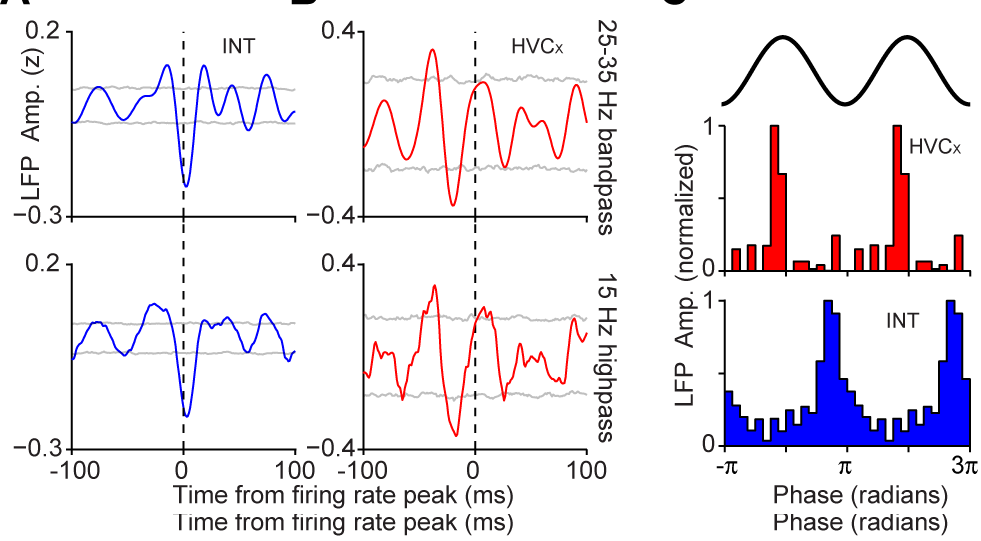
\includegraphics[width=11cm]{chapter4/figure8.png}
    \centering
\medskip
\caption[Spike-field analysis reveals an alternating 30 Hz rhythm in excitatory and inhibitory cells.  ]{\footnotesize \textbf{Spike-field analysis reveals an alternating 30 Hz rhythm in excitatory and inhibitory cells.}  \textbf{a}, Burst-triggered averages of 25-35 Hz (top row) and broadband LFPs (bottom) for interneurons (n=65, p=0, bootstrap test, see Materials and Methods) and \textbf{(b)} HVC$_{X}$ neurons (n=12, p=.006, bootstrap test). Gray line indicates p=.05. \textbf{c}, Here, the power of the LFP is binned at the phase of the LFP for each burst time.  A clear separation in preferred phase can be seen between HVC$_{X}$ neurons and interneurons. }

\label{fig:Sampling}
\end{figure}


These observations indicate that the phase of the 30 Hz LFP is highly correlated with firing times in two cell classes in HVC, and suggests that HVC$_{X}$ neurons, on average, fire during gaps in local inhibition. Anecdotally, within 16 channel carbon fiber bundles localized to volumes of 200 $\mu$m, we have observed multiple interneurons that produce correlated firing patterns and occasional synchronous pauses in inhibition across cells (Figure 4$\cdot$7a).  More rigorously, we find that interneuron troughs that occur within song syllables are more synchronous than one would expect by chance (median correlation coefficient .3848, .2895-.4652 99\% bootstrap confidence interval; p=0, bootstrap test, n=71 interneuron pairs, see Materials and Methods). This analysis was restricted to periods of time when the bird was actively producing sound. As a result, this analysis is not dominated by any modulations in firing rates related to the pattern of sound and silence that occurs within a song motif. Since the precise locations of the carbon fiber electrode tips were not known, we could not relate the degree of correlation to the spatial separation of interneurons. Synchronous pauses in inhibition could be responsible for the dips in the LFP, and could also provide a 'window of opportunity' for projection neurons to fire. At least one class of projection neuron, the HVC$_{X}$ neuron, tends to fire out of phase with inhibition in a 30 Hz time scale.


\section{Discussion}

In singing birds, the relationship between time and space in premotor cortical area HVC is neither random, nor globally organized as a traveling wave, but clustered on a 100 $\mu$m length scale. A 30 Hz rhythm revealed in the LFP and correlated with inhibition influences the timing of at least one projection neuron sub-type (HVC$_{X}$) , and this rhythm is coherent over a length-scale matching that of projection neuron calcium activity (Figure 4$\cdot$6).

The mesoscopic pattern apparent in the LFP and calcium imaging has not been observable using prior methods of sampling single cell activity serially. The stereotyped behavior of the songbird has allowed for alignment of multiple renditions of song, and the construction of 'pseudo-ensembles' based on populations of cells that were not simultaneously recorded \cite{Kozhevnikov:2007eu}. This approach has proven to be powerful in the song system, and has led to rapid advances in understanding the song circuit, but it is an approach that cannot resolve microcircuit dynamics in small volumes of HVC, and cannot resolve spatial maps on the length scale described here.  For lack of experimental data, prior dynamical models of HVC have not considered local spatial correlations in time cell firing {Long:2010db}. Most models also ignore the contribution of inhibitory interneurons \cite{Li:2006vz}, or assume that inhibition guards against runaway excitation {Long:2010db}, but is otherwise uninvolved in shaping projection neuron firing times (though there are a few notable exceptions \cite{Gibb:2009eu, Bertram:2014hd}).

In contrast, we find that the local microcircuit patterns in HVC in singing birds include correlations over space, and specific rules for the relative timing of distinct cell types. Our results reveal that HVC contains 'time domains' characterized by nearly synchronous projection neuron calcium activity. The 100 $\mu$m correlation length of the projection neurons also appears in the 30 Hz LFP, a signal that is highly correlated with an inhibitory rhythm expressed locally in HVC (Figure 4$\cdot$4b-c, and Figure 4$\cdot$8a). Within a local patch of HVC, the LFP and spike correlations indicate that, on average, HVC$_{X}$ projection neurons fire in gaps of inhibition (Figure 4$\cdot$8b). Taken together, these results indicate that functional domains within the HVC microcircuit may contain tightly correlated populations of excitatory and inhibitory cells that fire in opposition and generate a local 30 Hz rhythm in the LFP. These 'time domains' resemble the intermediate scale of geometric organization illustrated in Figure 4$\cdot$1b, characterized by zones in which projection neurons fire at similar times with no coherent global organization. 

Important questions remain about the microcircuit dynamics of HVC. Some are technical: the imaging results reported here rest on calcium imaging and the relationship between calcium transients and the underlying burst of action potentials in HVC projection neurons has not been measured during singing. At present, we can say that to first approximation the sparse calcium transients match the expected burst behavior of the excitatory cells in HVC. The head mounted microscope provided only single-color imaging, precluding cell type identification based on retrograde labeling of downstream targets. Similarly, the rhythm between HVC$_{X}$ cells and interneurons is inferred based on average timing relative to a common signal rather than direct measurements of connected pairs of cells.  Our electrophysiology did not address the relationship between HVC$_{RA}$ projection neurons and the inhibitory rhythm. The role each cell type in HVC plays in driving or responding to the local inhibitory rhythm, and the connectivity that gives rise to this rhythm, await more detailed description \cite{Mooney:2000ta, Mooney:2005db}. Moreover, neither the imaging nor the electrophysiology could directly measure the correlation length of the inhibitory neurons. This was extrapolated from the de-phasing length scale of the 30 Hz LFP, a measure clearly related to interneuron firing patterns, but still an imperfect surrogate.
	
Perhaps more interesting are the outstanding questions about the nature of a dynamical system governed by the properties observed here. Inhibitory neurons show patterned activity throughout song, whereas projection neurons fire sparsely, with calcium events that are correlated in time between neighbors. This suggests a microcircuit in which multiple pools of excitatory neurons drive local interneuron populations.  Then, in a feedback loop, locally synchronized inhibition on a 30 ms time-scale also influences the firing times of multiple pools of excitatory neurons. Theoretical models of neural sequence generation have focussed on the direct interactions between excitatory neurons, but our results suggest that the indirect interactions between excitatory neurons, mediated through inhibition, may be important in defining which cells fire at a given time. In this view, the timing of a projection neuron's activity may be defined not only by its connections to other projection neurons, but also by rhythmic patterns of inhibition dominated by a 30 Hz time-scale. Considering the importance of excitatory-inhibitory coupling in defining the timing of at least one class of projection neuron in HVC, the space of possible models for HVC activity expands significantly.

HVC is one stage in a motor cortico-thalamic loop, and intriguingly the time-scale of activity propagation around this loop is similar to the 30 Hz rhythm described here \cite{Ashmore:2008fy}. Future work is needed to examine whether this time-scale is intrinsic to cellular biophysics in HVC or arises from the time it takes excitatory pulses to propagate around the cortico-thalamic loop \cite{Hamaguchi:2012wj}. Whether this 30 ms time-scale is related to acoustic transitions in song remain to be examined \cite{Gardner:2001jn, Amador:2013ej} and will require more extensive sampling of excitatory and inhibitory cells over the entire volume of HVC. 

Functional clustering in HVC has been described previously in the spontaneous activity of anesthetized songbirds \cite{Graber:2013bq}, but we note a possible difference in the length scale reported in the spontaneous activity of anesthetized birds ($\lambda$=263 $\mu$m) and the length scale we observe in singing birds ($\lambda$=104 $\mu$m for calcium imaging, $\lambda$=108-125 $\mu$m for LFPs). The length scale of correlation during singing matches functional clustering on a 100 $\mu$m length scale that has been observed in mammalian motor cortex in the context of running, grooming \cite{Dombeck:2009cd}, and simple forelimb movements \cite{Hira:2013et, Peters:2014dq}.  Additionally, the 30 Hz rhythm has parallels in primate motor control \cite{Murthy:1992vu, Rubino:2006dd, Bartolo:2014ec} and speech perception and production in humans \cite{Giraud:2007ig}. The recurrence of these length scales and rhythmic time-scales across species and contexts raises the possibility that spatial clustering and 30 Hz rhythmic alternation of excitatory and inhibitory cells may be a recurring feature of cortical motor microcircuits and critical for the sequential organization of behavior. If true, this would imply that relatively slow movements produced by primates and the fast vocal movements of a songbird are coarse-grained in a similar fundamental length-scale (100 $\mu$m) and time-scale (30 Hz) at the level of cortical control.

For studies of songbird vocal learning, these results suggest that future biophysical models of motor sequence generation in HVC should move away from abstract models of neuronal chains defined only by the topology of excitatory cells, to consider new classes of models in which the interplay of spatially correlated patterns of excitation and inhibition form the basis of the stereotyped, robust sequences of neural activity driving birdsong.



\section{Materials and Methods:}

\subsection{Subjects}
All procedures were approved by the Institutional Animal Care and Use Committee of Boston University (protocol numbers 09-007 and 11-027).  Electrophysiology data were collected from 27 adult male zebra finches ($>$120 DPH), and imaging data were collected from 9 adult male zebra finches.  Bird were kept on a 14 hr light-dark cycle. 

\subsection{Viral labeling and calcium imaging.}

Chronic calcium imaging was performed using a head mounted fluorescent microscope described in detail elsewhere \cite{Ziv:2013fd}. To label HVC neurons with GCaAMP6s calcium indicator, birds received four 250 nl injections of lentivirus packaged with GcAMP6s under an Rous sarcoma virus (RSV) promoter into HVC \cite{Scott:2005gr}. To guide the injection of virus, the bounds of HVC were determined by bipolar antidromic stimulation of Area X (n=3) or through fluorescence imaging of a DiI retrograde tracer (n=6) \cite{Scott:2012gq}. We collected 167 ROIs from 9 birds. Fluorescent traces for each animal were collected over a single day of imaging.  For the calcium imaging, all songs were directed (i.e. a female was present).   

Our unpublished results indicate that the RSV promoter in HVC does not label interneurons or glial cells.  We have infected HVC with viruses with the RSV promoter driving transcription of several genes fused to GFP and performed double immunocytochemistry against GFP and several markers for inhibitory interneurons (parvalbumin, somatostatin and calretinin).  We did not observe co-localization of cells labeled with GFP with any of the interneuronal markers.  In addition, we also observed that the morphology of the GFP-positive cells was consistent with that previously described for projection neurons in HVC, but not consistent with them being glial cells. This observation suggests that the RSV promoter labels projection neurons in HVC.

GFP immunolabeling and confocal imaging of the RSV-GCaMP6s construct used here revealed that in all cases where dendrites were visible they contained spines, consistent with the morphology of HVC$_{RA}$ and HVC$_{X}$ projection neurons. Thirty percent of all infected neurons were HVC$_{X}$ projection neurons, based on retrograde labeling from Area X. Retrograde labeling was not performed from RA, but GFP immunolabeling revealed dense axon arbors in nucleus RA, indicating that a significant number of HVC$_{RA}$ neurons were also labelled.


\subsection{Electrophysiology.}

Electrophysiological recordings were gathered from 27 birds, where 13 received implants from 16-channel carbon fiber bundles, 5 from four 4-channel carbon fiber bundles, 3 from tungsten microwire arrays (Tucker Davis Technologies, 16-channel 33 $\mu$m wire diameter), and 6 from four-shank silicon probes (n=4 along the mediolateral axis, n=2 along the anterior-posterior, Neuronexus model no. A4x4-3mm-50-125-703-CM16, 15 $\mu$m thickness).  All arrays were implanted .7 mm anterior and 2.3 mm lateral of the midsagittal sinus at a depth of .4-.7 mm (head angle 30$^{\circ}$) using previously described methods \cite{Guitchounts:2013bs}.  All songs used  for electrophysiology were undirected (i.e. no female was present).  In a subset of the implants the position of the implant (but not single units) was verified antidromically with bipolar stimulating electrodes placed in Area X \cite{Hahnloser:2002hj}. Excitatory projection neurons and putative interneurons were identified based on their unique firing properties. In previous studies, antidromically identified HVC$_{X}$ projection neurons were shown to produce two more sparse, time locked bursts per motif. Putative interneurons produced dense, tonically active, time-locked firing patterns \cite{Hahnloser:2002hj}. All neurons reported in this study fell into one of these two categories.  Local field potentials (LFPs) were extracted from the same electrodes used to record single units after spike removal, and all statements about spike-field relationships were also confirmed with an analysis in which the LFPs were extracted from nearby electrodes, indicating that no cross-contamination between spikes and fields influenced these results.


\subsection{ Analysis of calcium imaging data}

All offline analyses of the calcium imaging data were performed using custom software written in MATLAB. First, the raw imaging data was motion corrected using a previously published algorithm \cite{GuizarSicairos:2008vj}.  Regions of interest (ROIs) were then manually selected and converted into single cell fluorescence traces by taking the mean intensity of all pixels within a given ROI for each movie frame. Baseline fluorescence for each trace, , was computed by taking the 12th percentile in an 800 ms sliding window (400 ms at each time point).  Changes in fluorescence were then defined as , where F is the fluorescence of a given ROI and a particular point in time.  Event times were computed by first finding all local peaks in the  trace that exceeded 1\%.  Events were excluded if   did not remain above -1\% for 300 ms after the detected peak.  Then, the event time was defined as the 50\% rise time between the peak and the preceding trough \cite{Ziv:2013fd}.  To provide an upper bound on the false positive rate given these criteria, which were chosen manually based on visual inspection of the data, we computed the likelihood of finding a peak when the birds were not singing (p=.0156 from 61.5 seconds of silence). All spatial correlations were computed using these event times, derived from temporally sparse fluorescence transients in spatially sparse  populations of infected neurons. The correlation length-scales calculated from these event times are robust to any out of focus fluorescence or neuropil signal that could add spurious correlations to the calcium time series. 

We also note that the distance measurements used for the spatial correlations are exact only if the imaged cells are all in the same plane, which is not the case here. The depth of each cell could not be determined since the head mounted cameras were used in a fixed location. To estimate the error due to this ambiguity, we focused the microscope sharply on 1 $\mu$m beads in agarose, and then defocused until the image of a bead expanded to the size of the largest selected ROI.  This provides a conservative measurement of how far outside the imaging plane a cell can be while still meeting the selection criteria of an ROI.  A more realistic measure was computed by defocusing from a spot the same size as the smallest ROI until it was distorted the same size as the largest ROI. By the conservative measure, cells that appear overlapping in the XY plane may be separated by a z-axis distance of 35 $\mu$m (22 $\mu$m by the more realistic measure). However, the true ambiguity in the euclidian cell to cell distance, taking into account the ambiguity in the Z plane, will decrease as ROIs appear more distant in the XY plane. Cells observed to be 50 $\mu$m apart will have an uncertainty of 11 $\mu$m (4.5 $\mu$m);  at 100 $\mu$m, the uncertainty is only 6 $\mu$m (2.4 $\mu$m).  



\subsection{Bootstrap tests of imaging data.}

The analyses shown in Figure 4$\cdot$2f-g were all conducted using randomization tests.  For Figure 4$\cdot$2f, the median distance between ROIs was plotted against the time between their respective calcium events.  To test for significance at each time bin, the same number of ROIs were randomly selected from the entire data set 10,000 times, and the median was computed for each randomization.  The p-value is then the probability that a median value from the randomized distribution is lower than the observed median. In Figure 4$\cdot$2g, the same procedure was used to test the length of the resultant vector.  That is, we tested whether the length of the resultant vector was longer than would be expected using the same randomization. Finally, ee used a similar procedure to test for the significance of the standard deviation of the anterior-posterior and mediolateral distance distributions. 

\subsection{Analysis of electrophysiology data}
Extracellular voltage traces were multiplexed and digitized at 25 kHz on the headstage and transferred to a PC over USB (Intan RHA2000).  Song was recorded using a head-mounted microphone glued to the headstage \cite{Guitchounts:2013bs}.  All offline analyses were performed using custom software written in MATLAB (Mathworks). To isolate single units offline, the extracellular voltage traces were bandpass filtered between 600 and 11000 Hz (12th order Elliptic filer, .2 dB passband ripple, 40 dB stopband attenuation) and sorted using standard offline spike sorting techniques \cite{Sahani:1999vj, Tolias:2007dy}. For the LFPs, voltage traces were first median filtered (1 ms window) to remove spikes \cite{Pesaran:2008gk}, then lowpass filtered with a 400 Hz corner frequency (4th order Butterworth filter) and downsampled to 1 kHz.  To isolate the 25-35 Hz LFP, the downsampled LFP was bandpass filtered between 25-35 Hz (149 tap Kaiser window FIR filter, 40 dB stopband attenuation, .05 ripple).  To minimize the impulse response, a more lenient 25-35 Hz bandpass was used for the spike-triggered analysis shown in Figure 8a-b (top) and for the comparison shown in Figure 4c (53 tap Kaiser window FIR filter, 20 dB stopband attenuation, .05 ripple). All event-triggered LFP analyses were also repeated using only a 15 Hz highpass filter (Figure 4$\cdot$8a-b bottom; 84 tap Kaiser window FIR filter, 20 dB stopband attenuation, .5 ripple). All filtering was performed forwards and backwards to correct for phase distortion.  Songs were aligned using previously described methods \cite{Poole:2012im}.  Spike-field coherence was estimated using standard techniques based on the cross-spectrum between the spike train and the LFP \cite{Jarvis:2001vr} (1 Slepian taper, NW=1).  To control for bias, the same number of trials were used for each neuron.  Additionally, we only included high quality single units for measuring spike field coherence (n=17 interneurons, SNR$>$8 and $<$.1\% ISIs $<$1ms, no sign of cluster contamination),  all other measures included all interneurons.    

\subsection{Song alignments}
 Songs were aligned using previously described methods \cite{Poole:2012im}. In brief, trials were aligned to song by computing the Euclidean distance in spectral features between the data and a template song in a sliding window. Troughs in the distance were considered candidate matches, and the spectral features of all potential hits were plotted in 2 dimensions and the user performed a cluster cut.


\subsection{Spike sorting. }

 First, positive and negative-going threshold crossings in the 600-11000 Hz bandpassed extracellular voltage traces were detected. The threshold was set to four times the bandpassed signal's robust standard deviation \cite{Quiroga:2004jc}. Then, a 1.1 ms window centered on the negative peak was saved. The spikes were then re-aligned to the negative peak after upsampling by a factor of 8 using cubic splines. Features of the aligned spike windows were computed using robust principal components analysis \cite{Sahani:1999vj}. A mixture of Gaussians model was fit to the spike features using the split and merge expectation maximization algorithm \cite{Tolias:2007dy}, and the number of components in the mixture was determined by fitting models with 2-7 components and choosing the model with the minimum Bayes Information Criterion \cite{Tolias:2007dy}. Unit quality was then assessed by signal-to-noise ratio and refractory period violations. For multi-unit analysis all threshold crossings above 3 standard deviations of the bandpassed signal were included.
 
 \subsection{Spectral density images}
 
 To compute the spectral density image for multiple aligned renditions of the same LFP, we used previously described methods \cite{Markowitz:2013ip}. First, a sparse, binary time-frequency representation of each rendition was generated using 'auditory contours' {Lim:2012uh}. Then, the binary representations were combined by summing across all renditions. In this representation, a false-color plot (Figure 4$\cdot$3a bottom) represents the probability of a binary contour passing through a given point in the time-frequency plane.

\subsection{Identifying bursts in projection neurons and interneurons for burst-triggered averaging. }

To identify bursts of single-unit activity, we first estimated the smooth firing rate for each trial using a Gaussian kernel ($\sigma$ = 5 ms). The smooth firing rate was averaged across trials, and we counted peaks above 100 Hz as burst events.

\subsection {Computing firing pattern distance}
We define the distance between two firing patterns as the mean absolute difference between their average firing rates. The firing rate was estimated by computing the smooth firing rate for each trial (Gaussian kernel, $\sigma$ = 5 ms ), and then averaging across trials. 

\subsection{Determining whether interneuron troughs are synchronous.}
To determine whether interneuron troughs within syllables were more coherent than one would expect by chance, we conducted a bootstrap procedure.  First, the firing rate was estimated within syllables by computing the smooth firing rate for each trial (Gaussian kernel, $\sigma$ = 5 ms ), averaging across trials, and z-scoring the average.  All negative-going peaks less than -.5 were counted as troughs.  A binary vector was created with 1s indicating the presence of a trough and 0s denoting all other time points (troughs in inter-syllable gaps were excluded), and each vector was smoothed with a Gaussian kernel $\sigma$ = 5 ms.  Then we computed the Pearson correlation coefficient between these smoothed vectors from all pairs of interneurons from the same bird (carbon implants only, n=71 pairs).  The median correlation coefficient across all birds was then compared to a null distribution estimated using a bootstrap procedure in which the troughs were selected randomly from time points during syllables (n=1000 bootstraps).

\subsection{Phase locking.} 
All phase locking indices (PLIs) were computed using previously described methods \cite{Lachaux:1999wt}.

\subsection{Statistical tests}
No formal methods were used to pre-determine sample sizes, but the sample sizes used here are similar to those generally used in the field. All statistical comparisons were performed using either a one-tailed or two-tailed Wilcoxon ranksum test with four exceptions.  First, the significance of the imaging results was determined using a bootstrap procedure (Figure 4$\cdot$2f-g, described above). Second, the significance of spike-field coherence (Figure 4b) was determined using a bootstrap procedure by shifting the spike trains across all trials by a separate random number for each neuron (1000 bootstraps). Third, the significance of burst-triggered average LFPs was computed using a bootstrap procedure.  Burst times were randomized for each neuron (1000 bootstraps), and the maximum absolute value was compared between the observed burst-triggered average and the bootstraps. Finally, the statistical significance of the trough timing was determined using a bootstrap where the troughs were randomly selected from time points during syllables (1000 bootstraps). Where appropriate, we controlled for multiple comparisons using the Bonferroni correction.     




%%==============[ CHAPTER 6 ]===============%%

\chapter{Unstable neurons underlie a stable learned behavior}
\label{chapter:body}

This chapter is a reproduction of previously published work (Liberti et al., 2016), and contains critical contributions from \emph{Dr. Jeffrey Markowitz}, who is an equal co-author on this manuscript. 

\section{Introduction}   
  
  Questions about coding stability at the single neuron level have been notoriously difficult to address given the challenge of stably recording from single neurons using implanted electrodes. In the hippocampus, earlier methods tracking tens of cells emphasized stable neural tuning over a timescale of a week \cite{Thompson:1990vj, Kentros:2004wq}, whereas recent studies tracking thousands of cells using new optical techniques \cite{Ghosh:2011ee, Chen:2013fc} revealed that 75-85\% of the cells change their tuning properties within the same timeframe \cite{Ziv:2013fd}. In whisker motor cortex, individual neurons in mice trained on an object detection task were unstable, but the relationship between ensemble measurements and behavior remained stable \cite{Huber:2012fw}. These studies support the view that for stable behaviors, individual neurons involved can show substantial drift in their tuning properties. 
For motor systems, the stability of neural tuning is not necessarily expected; the convergence of vast numbers of neurons in motor cortex to relatively few muscles \cite{Leonardo:2005bn} suggests that a given muscular activation pattern could be produced by many patterns of neural activity \cite{Rokni:2007fh}. In parallel, single neurons in motor cortex are observed to switch tuning properties in a task-dependent manner \cite{Ganguly:2009in}. In the case of the zebra finch, the precise timing and acoustic structure of song is preserved for years \cite{Immelmann:1969uh, Lombardino:2000vc}. Since the zebra finch sings a single song over the course of his lifetime, the question of neural coding stability is particularly well-defined. In the pre-motor cortical area that drives song, HVC (used as a proper name), three primary classes of neurons can be found: inhibitory interneurons, basal-ganglia projecting neurons (HVC$_{X}$), and motor projecting neurons (HVC$_{RA}$).  A third projection neuron type HVC$_{AV}$ sparsely populates the nucleus, but its activity has not yet been described in singing birds \cite{Mooney:2014tn}.  In HVC, each neuron type that has been observed produces a highly stereotyped pattern of action potentials, and these patterns are stable over the time intervals that they have been recorded: minutes to hours \cite{Hahnloser:2002hj, Kozhevnikov:2007eu}. For inhibitory interneurons, the pattern is dense, with spikes occurring throughout song \cite{Kozhevnikov:2007eu, Guitchounts:2013bs}. In contrast, excitatory projection neurons that communicate with downstream targets fire 'ultra sparsely' \cite{Hahnloser:2002hj}. 

During song production, HVC$_{X}$ neurons and inhibitory interneurons exhibit cell-type specific phase-locking to the local field potential (LFP) at 30 Hz. HVC$_{X}$ cells fire in the peak of the LFP and interneurons in the trough \cite{Markowitz:2015ko}. Intracellular recordings in vitro and in vivo suggest that HVC$_{RA}$ neurons also fire in gaps of inhibition \cite{Kosche:2014wu}. Moreover, both the LFP and projection neuron activity are clustered over a 100 $\mu$m length-scale. The phase locking relationship between excitatory and inhibitory neurons is only observed with multiple neuron recordings in the same small volume/phase shifts across HVC preclude a global rhythmic relationship among cell types \cite{Lynch:2016jb}. Taken together, these observations indicate that spatially coherent mesoscopic patterns of inhibition underlie HVC dynamics, where synchronous gaps in local interneuron population activity control projection neuron timing. 

\begin{figure}[!htb]
 %\begin{minipage}[t]{0.49\linewidth}\centering
    \includegraphics[width=11cm]{chapter5/figure1.png}
    \centering
\medskip
\caption[Approach to measuring the stability of neural firing patterns underlying a highly stable behavior.]{\footnotesize \textbf{Approach to measuring the stability of neural firing patterns underlying a highly stable behavior.} \textbf{A}, Spectral density images, for the songs sung by the same bird 405 days apart (n=1412 songs for Day 1 and n=1480 songs for Day 405). \textbf{B}, To measure projection neuron stability a head mounted fluorescence microscope was used to image GCaMP6 delivered by a cell-type specific virus. \textbf{C}, Stability of multi-unit and inhibitory interneuron activity patterns was measured using a custom carbon fiber electrode array.}

\label{fig:Sampling}
\end{figure}

The recent evidence in support of locally organized ensemble activity in HVC allows us to raise the following question: What explains the persistence of the song motor pattern, single neuron stability, or stability of ensemble dynamics. A recent experiment suggests that HVC ensemble dynamics measured through multi-unit activity \cite{Crandall:2007ke} is resilient to circuit perturbations \cite{Otchy:2015hq}. Here we extend the observation of HVC ensemble dynamics using new electrophysiological \cite{Guitchounts:2013bs} and imaging methods (Figure 5$\cdot$1b,c) to address the stability of excitatory projection neurons.


\section{Results}
\subsection{Song is supported by stable mesoscopic dynamics}

\begin{figure}[!htb]
 %\begin{minipage}[t]{0.49\linewidth}\centering
    \includegraphics[width=13cm]{chapter5/figure2.png}
    \centering
\medskip
\caption[Activity patterns from multi-unit ensembles and single interneurons are highly stable.]{\footnotesize \textbf{Activity patterns from multi-unit ensembles and single interneurons are highly stable.} \textbf{A-C} Burst-triggered averages of 25-35 Hz Local Field Potentials (LFPs) for HVC$_{X}$ neurons \textbf{(A)}, interneurons \textbf{(B)}, and multi-unit activity \textbf{(C)}. \textbf{D-F}, The power of the LFP is binned at the phase of the LFP for each burst time. A clear separation in preferred phase can be seen between HVC$_{X}$ neurons \textbf{(D)} and interneurons \textbf{(E)}, but not between interneurons and multiunit activity (F). G, Trial-averaged band-passed LFPs (25-35 Hz) from a single electrode up to 495 days post-implant. \textbf{H}, Examples of multiunit stability over month-long timescales. \textbf{I-J}, Multi-unit patterns are stable over 40 days measured using patterns in firing rate \textbf{(I)} or root-mean-square (RMS) \textbf{(J)} values are stable over 40 days (inset, over 120 days). Colors indicate different birds, many are not visible due to overlap in the upper-left portion of the plot. \textbf{K}, Inhibitory interneuron firing patterns are stable for up to 124 days. Average waveforms are shown next to the corresponding raster (red shading indicates standard deviation).}

\label{fig:Sampling}
\end{figure}

Local field potentials (LFPs) can reflect the synchronous activity of neural ensembles over a length-scale of approximately 100 $\mu$m \cite{Katzner:2009gp} (though see \cite{Buzsaki:2012db}). We recorded LFPs in the zebra finch pre-motor cortex (HVC) using both commercial and previously-described custom carbon fiber electrode arrays \cite{Guitchounts:2013bs, Markowitz:2015ko}. The phase of the 30 Hz LFP is coherent with the spiking of HVC interneurons and projection neurons (Figure 5$\cdot$2a-f) \cite{Markowitz:2015ko}; we found this local phase was precisely conserved over long timescales (Figure 5$\cdot$2g). For most of our implants we were able to record the LFP for up to 30 days, and we found that over this timescale the 30 Hz phase exhibited a drift of less than 0.25 radians or approximately 15 degrees (modal change of .244 radians over 30 days, .232-.254, 95\% bootstrap confidence interval, Extended Data Figure 5$\cdot$1a). This stability in LFP phase indicates that ensemble activity, reflecting a combination of local spiking and presynaptic inputs, does not undergo a major reconfiguration.  

\subsection{Multi-unit ensembles and single inhibitory neurons are stable}

While the LFP is thought to reflect ensemble activity from both excitatory and inhibitory neurons over a length-scale of approximately 100 $\mu$ms \cite{Markowitz:2015ko}, multi-unit recordings from large surface area electrodes can reflect the aggregate activity of tens of nearby neurons within a local volume. To monitor the stability of multi-unit activity, we implanted custom electrodes that were geometrically optimized for sampling from cells across the full depth of HVC. Figure 5$\cdot$2h reveals a multi-unit raster with detailed temporal structure in the pattern of firing and silence, with an average precision of 4.587 ms (4.348-4.843 ms, 95\% bootstrap confidence interval consistent with the stereotyped neural activity reported previously in HVC \cite{Schmidt:2003vb, Hahnloser:2002hj}. The neural patterns shown in Figure 5$\cdot$2h represent finely timed bursts of activity in an unknown number of cells (the number of simultaneously active cells recorded per electrode was more than could be separated by spike-sorting). However, spike-field measurements indicate that the multi-unit signal is phase-locked to the trough of the 30 Hz component of the LFP, suggesting that multi-unit signals are dominated by inhibitory interneurons (Figure 5$\cdot$2c,f) \cite{Markowitz:2015ko}. Enhanced representation of inhibitory cell activity in multi-unit signals is to be expected since projection neurons fire 'ultra-sparsely' \cite{Hahnloser:2002hj} and contribute many fewer spikes to a multi-unit signal than do interneurons. The suggestion drawn from multi-unit signals that pattens of inhibition are stable in HVC (Figure 5$\cdot$2h-j) was directly confirmed in long term recordings from n=6 inhibitory neurons from single unit recordings (3 are shown in Figure 5$\cdot$2k). As revealed in Figure 5$\cdot$2k, inhibitory neuron firing patterns were remarkably stable, even over a time-scale of months. In addition to the stability of the 30 Hz LFP phase, this result indicates that ensemble inhibitory activity is highly stable. 

\begin{figure}[!htb]
 %\begin{minipage}[t]{0.49\linewidth}\centering
    \includegraphics[width=12cm]{chapter5/figure3.png}
    \centering
\medskip
\caption[Drift in multi-unit firing patterns is not accelerated by unilateral TS nerve transection. ]{\footnotesize \textbf{Drift in multi-unit firing patterns is not accelerated by unilateral TS nerve transection.}  \textbf{A-B}, Representative sonogram and multiunit raster before (A) and after the TS nerve cut (B). \textbf{C-D}, Change in acoustic features after nerve cut (***, p$<$.001, Wilcoxon ranksum test). \textbf{E-F}, Post-nerve cut, multi-unit activity does not drift more than expected in the pre-cut baseline condition. Shown is the average correlation at each time point relative to the last baseline day. Blue indicates the 95\% confidence interval estimated from the baseline condition. 
}

\label{fig:Sampling}
\end{figure}

We next asked if the stability of this multi-unit activity depended on sensory feedback. Previous work has shown that the statistical distribution of post-synaptic potentials (PSPs) in HVC projection neurons is invariant to altered auditory feedback induced through a tracheosyringeal (TS) nerve cut \cite{Vallentin:2015hf}, but over long timescales, the song of the adult zebra finch is known to be maintained through an auditory-feedback dependent process \cite{Nordeen:1992fy, Tschida:2012ig}. We anticipated that the rate of drift in the ensemble pattern would increase with perturbations to auditory feedback. Following baseline recording, we severed the ipsilateral TS nerve that relays motor commands to the birds' vocal organ (n=5 birds). As in previous work \cite{Williams:1992fx, Vallentin:2015hf}, this loss of muscular control results in acoustic distortions of song (Figure 5$\cdot$3a-d, see Extended Data Figure 5$\cdot$2 for all examples), degrading the learned sensory-motor correspondence between vocal commands and auditory feedback. Following this, we monitored the song and HVC multi-unit firing patterns for a period of approximately one month. Over this time interval, song did not recover, and the multi-unit spike patterns in the pre-motor cortical zone HVC remained stable (Figure 5$\cdot$3e-f). In all birds subject to the TS cut, shifts in the firing pattern occur at the same rate as for baseline recordings (p$>$.05 for all birds, one-tailed Wilcoxon ranksum test). We conclude from this that the ensemble pattern in HVC is robust to changes in auditory feedback that result from unilateral TS nerve removal. Here the song is altered, but the detailed ensemble firing patterns persist in HVC as though no change had occurred. This observation is synergistic with a recent study showing resilience of the HVC ensemble pattern after neural circuit perturbations \cite{Otchy:2015hq}.


\subsection{Individual projection neurons are unstable over days.}

\begin{figure}[!htb]
 %\begin{minipage}[t]{0.49\linewidth}\centering
    \includegraphics[width=16cm]{chapter5/figure5.png}
    \centering
\medskip
\caption[Projection neurons drift over a five day imaging session ]{\footnotesize \textbf{Projection neurons drift over a five day imaging session} \textbf{A}, Images colored by the timing of max pixel intensity, for two birds, across 5 (\textit{top}, Inscopix microscope) and 4 (\textit{bottom},  custom microscope) day intervals. \textbf{B}, Trial-averaged activity from all song related neurons from one animal. Keeping the same sorting and amplitude color scale, the ROIs are plotted for 5 consecutive days. \textbf{C}, For the same animals shown in A, cells active on three consecutive days are combined in a single image where color now indicates neuron participation rather than timing. (red=day 1, blue=day 2, and green=day 3). Cells with persistent activity on all 3 days appear white in this representation (see Extended Data Fig 5). Cells that change amplitude or change firing probability appear colored. \textbf{D}.  Electrophysiological recording of a projection neuron reveals a new  song-locked burst that emerges over the course of a day. Blue triangles indicate trials plotted at the bottom of the figure. }
\label{fig:Sampling}
\end{figure}

Our electrophysiology methods were unable to track individual excitatory projection cells over time-scales longer than a single day, perhaps due to limitations of recording from smaller cells \cite{Guitchounts:2013bs}. To provide information about the stability of excitatory cells, we turned to optical imaging of genetically encoded calcium indicators (Figure 5$\cdot$4a, Extended Data Figure 5$\cdot$3) \cite{Markowitz:2015ko, Picardo:2016hv}. This was accomplished through the use of miniature head-mounted microscopes \cite{Ghosh:2011ee} using both a commercial head-mounted microscope (Inscopix, n=1 bird), and a custom 3D-printed microscope (3 birds) designed to promote freedom of movement in singing birds (Figure 5$\cdot$4 and Extended Data Figure 5$\cdot$4).  

\begin{figure}[!htb]
 %\begin{minipage}[t]{0.49\linewidth}\centering
    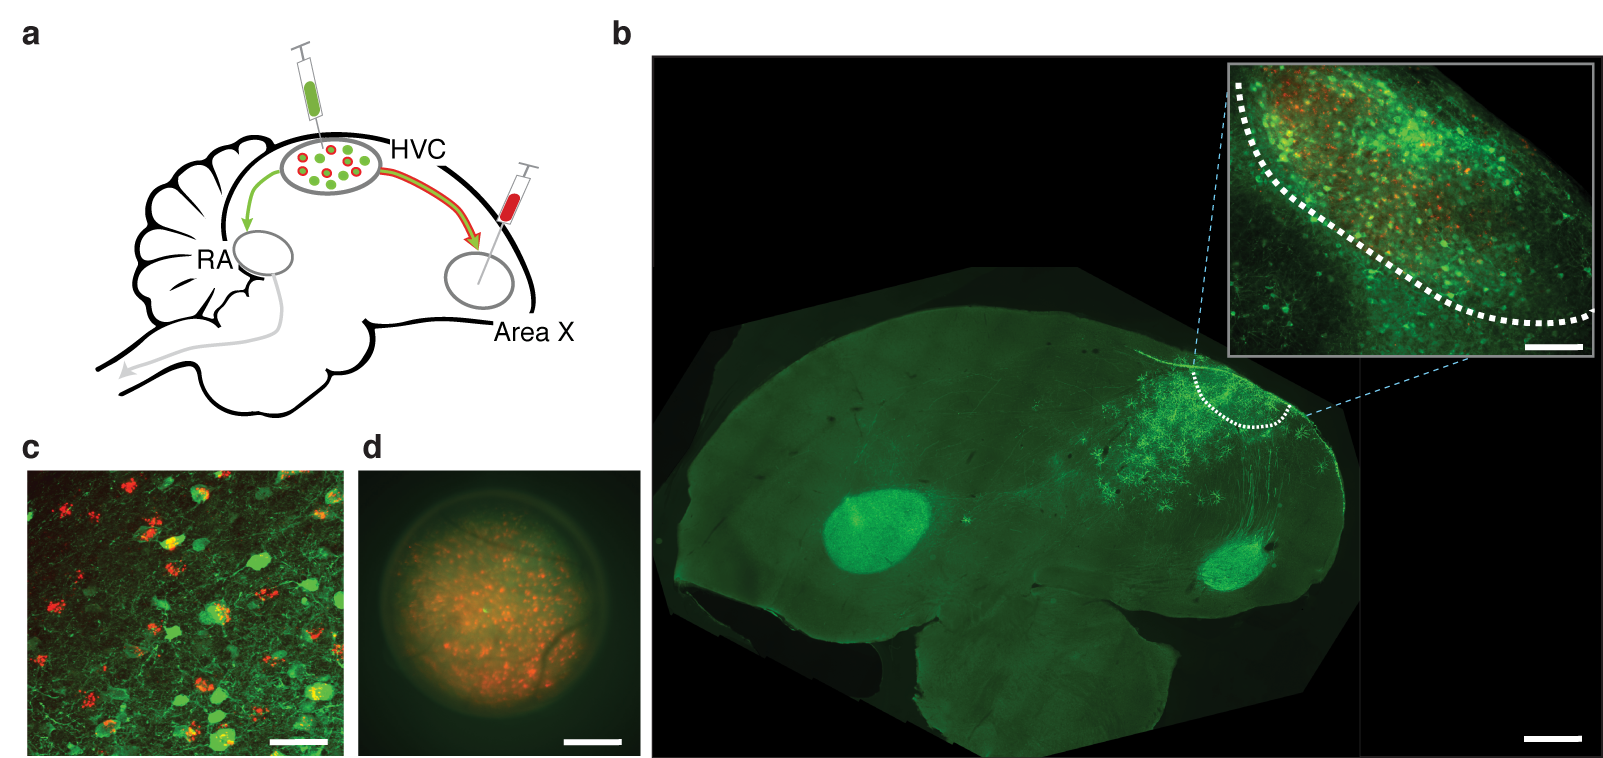
\includegraphics[width=15cm]{chapter5/figureS3.png}
    \centering
\medskip
\caption[Histological verification of virus used for calcium imaging. ]{\footnotesize \textbf{Histological verification of virus used for calcium imaging.} \textbf{A}, Diagram of experimental strategy for calcium imaging. Virus expressing GFP was injected into HVC, and a retrograde dye (DiI) was injected into the downstream nucleus Area X. \textbf{B}, Lentivirus with an RSV promoter produces dense infections of HVC projection neurons. Scale bar indicates 400 $\mu$m. \textit{Inset}, closeup of HVC, bounded by the white dotted line. Scale bar indicates 39 $\mu$m. \textbf{C}. Co-localization of GFP-expressing neurons in HVC and DiI backfill. Scale bar, 250 $\mu$m. \textbf{D}, View of HVC through a chronically implanted GRIN lens. Scale bar, 250um.}
\label{fig:Sampling}
\end{figure}



This microscope provided the first measurements of calcium activity during undirected singing; the solo practice song of the zebra finch.  Projection neuron calcium activity patterns were sparse and time-locked to singing (Figure 5$\cdot$4a). The timing of most projection neurons was stable over several days (Figure 5$\cdot$4a,b), however, across days, the probability that a given cell fires during singing can change dramatically (Figure 5$\cdot$4c, Figure 5$\cdot$7c). Across an interval of days, cells both drop out and newly appear in the song pattern (Figure 5$\cdot$5b,c, and Figure 5$\cdot$6-8). Stable and unstable ROIs can be found next to each other (Figure 5$\cdot$6,7). 

\begin{figure}[!htb]
 %\begin{minipage}[t]{0.49\linewidth}\centering
    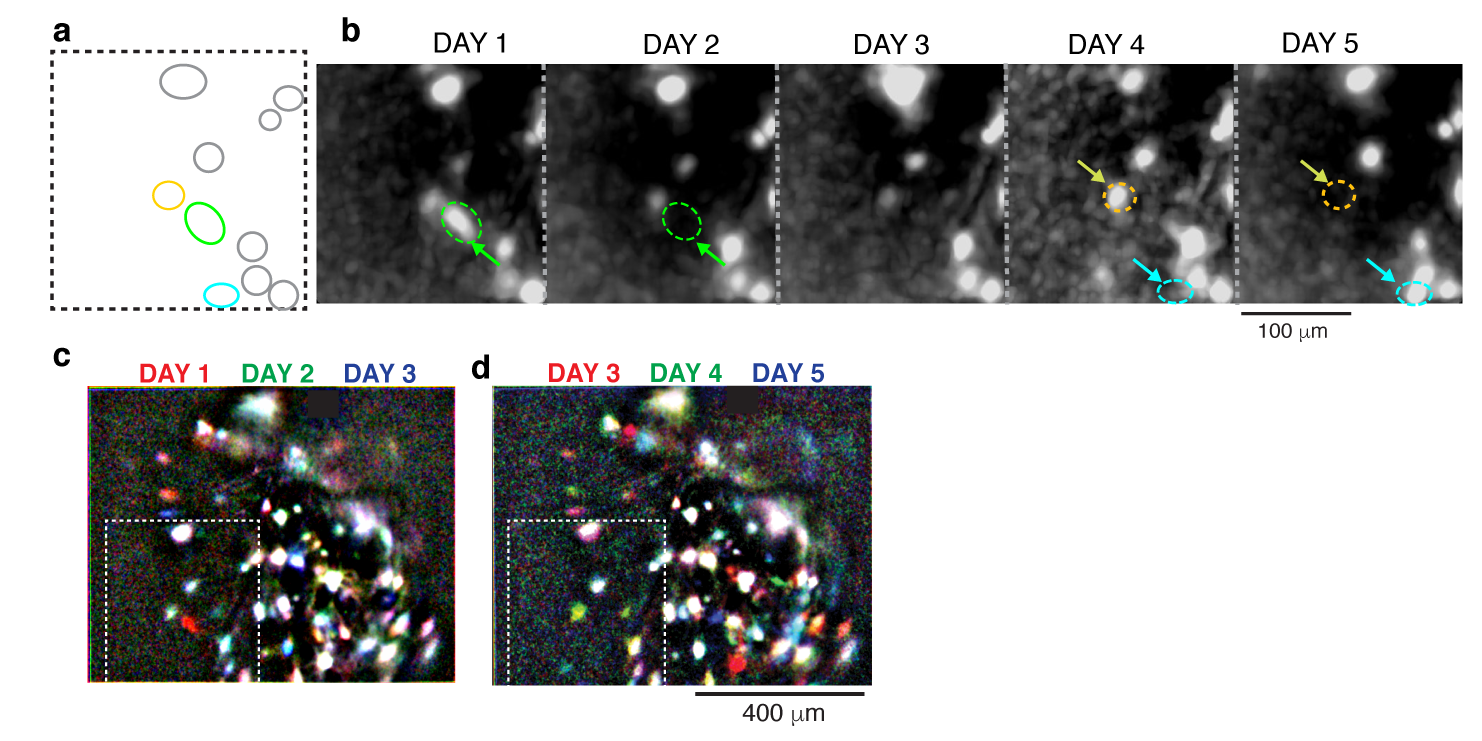
\includegraphics[width=15cm]{chapter5/figureS7.png}
    \centering
\medskip
\caption[Examples of stable and unstable cells in the same imaging region.]{\footnotesize \textbf{Examples of stable and unstable cells in the same imaging region.} \textbf{A}, ROI masks for cells in region. \textbf{B}, Maximum projection of a 191 x 203 $\mu$m subsection of the averaged, song-aligned calcium imaging movies, across 5 days. Arrows highlight two cells in this plane that either drop out (green, yellow) or in (blue) of the neural sequence across days. This region is a smaller section of the total imaging plane, shown in C and D. \textbf{C}. Three day maximum projection overlay from the data in Figure 5$\cdot$4C. The maximum projection image is divided by a smoothed version of the same image,using a 100 pixel disk filter, to normalize across bright and dim ROIs. \textbf{D},  The last three days of the five day longitudinal study, using the same normalization as in C}
\label{fig:Sampling}
\end{figure}

\begin{figure}[!htb]
 %\begin{minipage}[t]{0.49\linewidth}\centering
    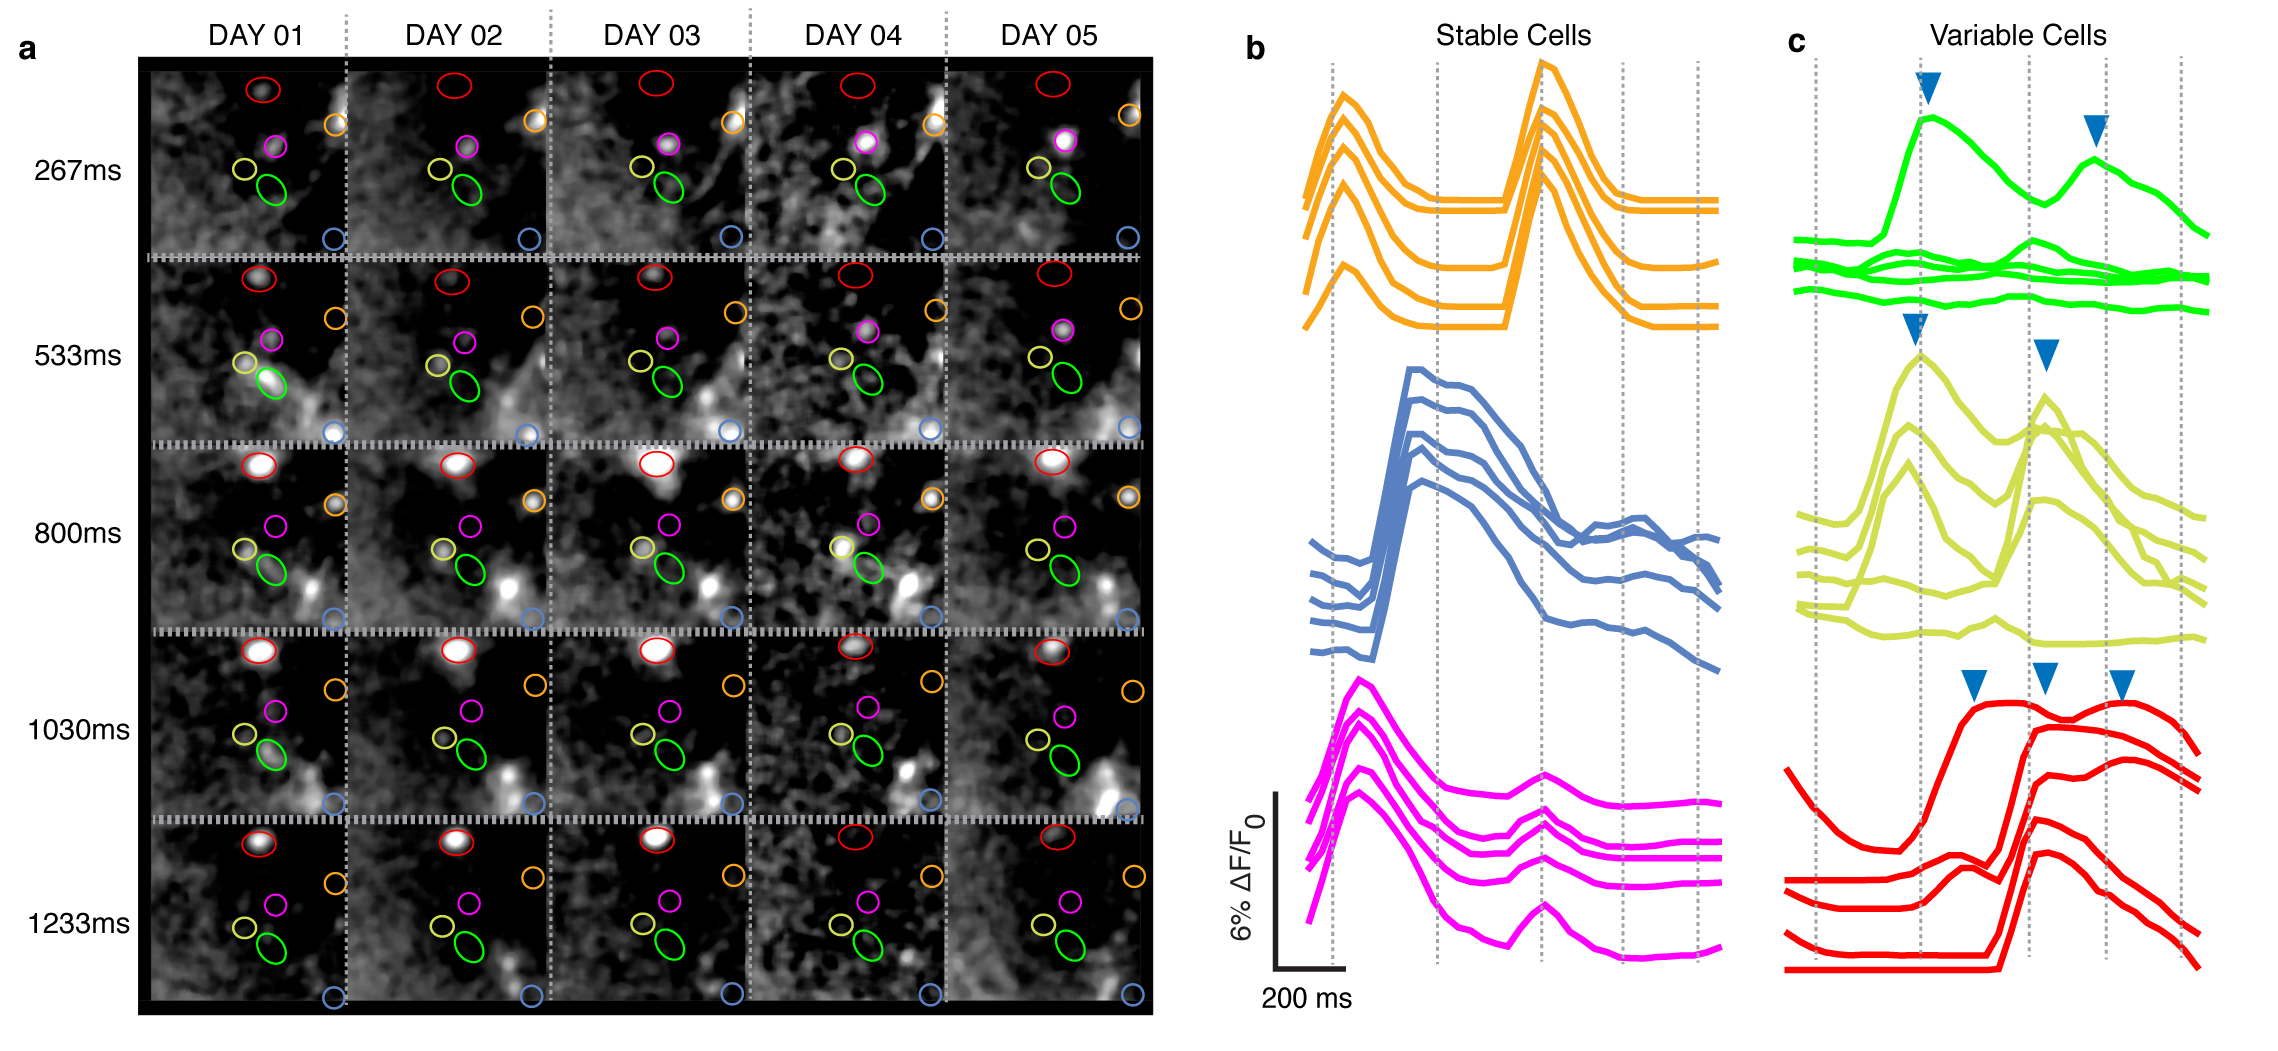
\includegraphics[width=15cm]{chapter5/figureS8.png}
    \centering
\medskip
\caption[Examples of amplitude traces from multi-peaked traces.]{\footnotesize \textbf{Examples of amplitude traces from multi-peaked traces.} \textbf{A}, Single frame stills from the trial-averaged, song-aligned calcium imaging movies, across all 5 days of a longitudinal study. Columns are days, and rows are frame times relative to the start of song. \textbf{B}, Example of three cells with stable timing and amplitude. Five traces represent five days (ordered top to bottom from day 1 to day 5.). \textbf{C}, Traces of three cells that are unstable across days, with triangles indicating calcium peak times. Dashed lines indicate times corresponding to each frame from A.}
\label{fig:Sampling}
\end{figure}
	
One class of projection neuron (HVC$_{X}$) can produce more than one time-locked burst of action potentials during singing. For cells with multiple timing peaks, amplitude or probability of activation could change independently for each peak. This was witnessed both in calcium imaging and in electrophysiological recordings. An example is the the 'fade-in' of a second burst time in a projection neuron recorded with a carbon fiber electrode over the course of a day (Figure 5$\cdot$5d).

For the imaging data, we performed analysis on two ROI sets: one analysis included all ROIs found on any day of imaging (ROIs$_{present some days}$). The second included only ROIs unambiguously present on all days of imaging (ROIs$_{present all days}$). By the fifth day of imaging, across all ROIs recorded, a large number of ROIs showed statistically significant changes in their mean song-aligned activity (p$<$.01 permutation test, 15/39 ROIs for bird 1, 27/38 for bird 2, 26/76 for bird 3 and 26/81 for bird 4, ROIs$_{present some days}$; 11/18, 14/16, 11/22, 5/21, ROIs$_{present all days}$).

\begin{figure}[!htb]
 %\begin{minipage}[t]{0.49\linewidth}\centering
    \includegraphics[width=12cm]{chapter5/figure6.png}
    \centering
\medskip
\caption[Projection neuron activity preferentially changes over periods of sleep. ]{\footnotesize \textbf{Projection neuron activity preferentially changes over periods of sleep.} \textbf{A}, Average correlation across all ROIs across different lags for each bird. Shaded region indicates 95\% bootstrap confidence interval. \textbf{B}, \textit{Top}, All correlations up to a lag of 4 days for multi-unit activity (n=20 birds, one sample per bird) and projection neuron activity (p=2.7e-6, z=4.70, one-tailed Wilcoxon ranksum test). Highlighted in red are cells that participate unambiguously across the entire time series ( p=9.8e-4, z=3.30 one-tailed Wilcoxon ranksum test). 
\textit{Bottom}, Cumulative density functions (CDF) of the data shown above: multiunit data in gray, projection neurons seen across all days in red, and seen clearly on any day are blue. \textbf{C}, The shift in correlation occurs primarily overnight (***, ROIs$_{present some days}$ p=2.0e-40, z=-13.26, ROIs$_{present all days}$ p=1.59e-14, z=-7.59, sign-rank test; shown are data from ROIs$_{present all days}$). \textbf{D}, Song consistency increases over the course of the day (r=.28, p=6.6e-8, Spearman rank correlation). \textbf{E}. Consistency in the timing of peak $\Delta F/F_{0}$ (measured over the whole song) increases with time of day (ROIs$_{present some days}$ r=.14 p=6.1e-9, ROIs$_{present all days}$ r=.18 p=9.7e-7, Spearman rank correlation,  shown are data from ROIs$_{present all days}$). F. The trial by trial correlation between calcium activity and the previous day's average also increases with time of day (ROIs$_{present some days}$ r=.12 p=5.6e-3, ROIs$_{present all days}$ r=.25 p=4.3e-9, Spearman rank correlation; shown are data from ROIs$_{present all days}$). All time of day measurements in E and F use only data our custom microscopes detailed in Figure 5$\cdot$4 (n 3 birds).}

\label{fig:Sampling}
\end{figure}

This shift in projection neuron activity across multiple days is inconsistent with their previously observed stability during brief, minutes-long recordings \cite{Hahnloser:2002hj, Long:2010db}. This contrast motivated us to examine whether the shift in projection neuron activity occurred primarily during the day or during the night. We found a much stronger shift in song-aligned projection neuron calcium traces after a night of sleep than over the course of a single day (Figure 5$\cdot$8c, Figure 5$\cdot$6, ROIs$_{present some days}$ p=2.0e-40, z=-13.26, ROIs$_{present all days}$ p=1.6e-14, -7.59, one-tailed sign-rank test). Next, we checked if drift could be accounted for by time elapsed. First, we analyzed whether calcium activity decreased in consistency across the day, and, surprisingly found the opposite to be true: consistency increased over the course of each day (Figure 5$\cdot$6e, ROIs$_{present some days}$ r=.14 p=6.1e-9, ROIs$_{present all days}$ r=.18, p=9.7e-7). We also found that song-aligned calcium activity became more similar to the previous day's average over the course of the day (Fig 6f, ROIs$_{present some days}$ r=.12, p=5.6e-3, ROIs$_{present all days}$ r=.25 p=4.3e-9, Spearman rank correlation). Thus, within each ROI, song-aligned calcium activity changes significantly over a night's sleep, and then recovers in both self-consistency and in similarity to previous day's average as the day progresses. Given these observations, the drift in calcium activity is not simply a function of time elapsed. Rather, these results suggest that sleep actively destabilizes the representation of song in pre-motor cortex area HVC.


\subsection{Close inspection reveals the fine microstructure of song also changes over intervals of sleep and increases in consistency throughout the day}

The finding that projection neuron activity is unstable across days prompted us to carefully quantify the microstructure of song behavior using a highly-sensitive time-frequency analysis method developed for analysis of sparse signals such as zebra finch song. The persistence of zebra finch song structure has been documented over timescales of years \cite{Immelmann:1969uh,Lombardino:2000vc} and as demonstrated in Figure 5$\cdot$1, over the period of a year, the song appears to be remarkably stable (Figure 5$\cdot$1A); however, the micro-structure of song is not precisely the same, even in this example. High resolution investigation of the microstructure reveals small but significant shifts over the interval of a week, and these changes occur primarily over periods of sleep (p=9.8e-4 w=55, one-tailed Wilcoxon ranksum test). Moreover, similar to the drift in calcium activity, we found that song consistency also increases over the course of the day (Figure 5$\cdot$8d, r=.28, p=6.6e-8, Spearman rank correlation. 


\section{Discussion}


This study suggests that memories encoded in cortex, like many structural features of the human body, undergo renewal at the cellular level. Skin maintains its shape despite the turnover of cells \cite{Weinstein:1965ka}, and the intestinal surface has constant turnover but maintains its function \cite{Creamer:1961jp}. For the stable song of the zebra finch, instability of the neural program qualitatively matches the microscopic day-to day changes in song, but the song changes observed over intervals of sleep are small, while the pattern of neuronal participation changes more dramatically. What explains the persistence of the song motor pattern in spite of the unstable projection neurons underlying song?

A key finding is that on a mesoscopic scale, the premotor cortical area HVC is stable. Over the length scales recorded in LFPs and multi-unit recordings (approximately 100 microns), the neural basis of song is largely unchanged over a timescale of weeks to years. In contrast, individual projection neurons drift: not primarily in the timing of their activity, as much as in the burst probability and participation in the song pattern. One potential factor contributing to ensemble stability in HVC is the spatial correlation observed in the firing patterns of excitatory cells. Nearby excitatory neurons in HVC fire at similar times, and the length-scale of this correlation is roughly 100 microns \cite{Markowitz:2015ko}. If individual projection neurons fade out of the ensemble, nearby projection neurons could be serving redundant roles.

A second related factor contributing to ensemble stability is the role of temporally patterned inhibition in HVC. In contrast to the instability of excitatory neuron coding, we have observed that inhibitory interneuron firing patterns are stable for weeks or months; for as long as it was technically possible to track the firing patterns of the cells. At the simplest level, excitatory neurons are postulated to be driven by a relatively sparse number of strong synapses, leading to the sparsity of their firing patterns \cite{Diesmann:1999in, Long:2010db}. Support for this prediction has been found from serial electron microscopy reconstruction of HVC \cite{Benezra:2015ux}. In contrast, many inhibitory interneurons in HVC have large dendritic arbors and are thought to be driven by a large number of presynaptic partners \cite{Mooney:2005db}. The prediction from HVC connectivity is that changes in a small number of synapses could alter the excitatory neuron firing patterns dramatically, but influence the inhibitory interneurons very little. In light of this numerical argument, and the observed stability of single inhibitory neurons, HVC ensemble patterns could be stabilized if interneurons have a strong local influence over projection neuron activity. Indeed, this appears to be the case. The firing times of the excitatory projection neurons coincide with stereotyped pauses in local inhibition \cite{Kosche:2014wu, Amador:2013ej}, and HVC$_{X}$ excitatory neurons and inhibitory interneurons fire in opposite phases of the 30Hz LFP \cite{Markowitz:2015ko}. The observations are true on the micro-scale, and due to phase shifts across the extent of HVC the rhythmic alternation is not observed globally \cite{Lynch:2016jb}. Local blockade of inhibition releases the sparse firing cells from inhibition and they begin to fire at multiple times in song \cite{Kosche:2014wu}. Building on these observations, a recent modeling study suggested that inhibitory interneuron dynamics can increase the robustness of HVC dynamics to added noise \cite{Cannon:2015jq}. These models can be made more precise in future experiments as additional cell type specific information is measured. The relative stability of different classes of HVC excitatory neurons (HVC$_{RA}$, HVC$_{X}$ and HVC$_{Av}$) remain to be examined since our methods could not distinguish among the three cell types. In the songbird, stable patterned inhibition may be an important force in maintaining the dynamical pattern of song in spite of underlying drift in the projection neurons. For mammals, similar principles may apply. Aspects of the song corticothalamic loop resemble features of mammalian motor cortex, including an important 30 Hz rhythm \cite{Markowitz:2015ko, Rubino:2006dd, Murthy:1992vu} and spatial correlations in neuron firing patterns over 100 $\mu$m length scales \cite{Dombeck:2009cd, Peters:2014dq, Hira:2013et}. In mammalian motor cortex, it will be interesting to track drift in excitatory versus inhibitory neuron populations to see if patterned inhibition may provide a stabilizing force in motor skill persistence. 

Finally, we address the importance of sleep in the rearrangement of the song code in HVC. The change in the song motor pattern occurs primarily over intervals of sleep, and we have shown that adult song behavior also undergoes microscopic shifts in sleep. Our results may be related to a previous observation: as juveniles learn to sing, their songs progress through a day of practice \cite{Ohgushi:2015kp}, but degrade slightly over intervals of sleep \cite{Deregnaucourt:2005kk}. The depth of this overnight 'backsliding' is positively correlated with the eventual success of song learning, indicating that nighttime song rearrangements are important for learning. In addition, if song-aligned HVC activity is disrupted through lesioning Nif, an area upstream of HVC, the pattern recovers primarily overnight \cite{Otchy:2015hq}. 
The present study provides a possible neural mechanism for these sleep effects, raising, the possibility that new patterns of activity 'invented' over intervals of sleep provide important raw material for song learning and maintenance.  Francis Crick proposed that noisy reactivation of neural circuits in sleep weakens the strongest pathways in the brain, promoting adaptive plasticity \cite{Crick:1983wa}. Songbirds reactivate their song patterns in pre-motor cortex in a noisy or incomplete manner \cite{Dave:2000wp} and it is possible that this spontaneous activity drives the overnight shift in HVC excitatory neurons observed here. Future studies can track the firing patterns of excitatory neurons in HVC while silencing or overstimulating spontaneous activity in sleep, directly testing the hypothesis that noisy replay of song in sleep promotes adaptive plasticity of the song motor program. It remains to be seen whether the overnight shift in HVC is random, or guided by vocal errors. Random shifts in the population could increase robustness of HVC dynamics by enforcing redundant representations of song. In contrast, shifts in the population that are influenced by vocal performance errors could be an active part of song learning and maintenance.


\section{Methods}
\subsection{Subjects}
All procedures were approved by the Institutional Animal Care and Use Committee of Boston University (protocol numbers 14-028 and 14-029). Electrophysiology data were collected from n=27 adult male zebra finches ($>$120 DPH), and imaging data were collected from n=4 adult male zebra finches. Birds were kept on a 14 h light-dark cycle.

\subsection{Splaying microfiber electrodes}
We used a previously-described minimally invasive carbon fiber electrode array \cite{Guitchounts:2013bs} in addition to commercially available arrays (TDT, Neuronexus) to chronically monitor both single units and LFPs. Extracellular voltages were amplified and digitized at either 25 or 30 Khz using the Intan acquisition system (RHA2000 and RHD2000).

\subsection{Microfiber electrodes for multi-unit recordings}
Bare (i.e. uncoated) microthread electrodes were prepared by extracting 5 and 11 $\mu$m diameter fibers from commercially available spools of carbon fiber (grade XAS, HTA, T300 or P25). Once extracted, sizing and other impurities were removed by heating fibers as previously described \cite{Guitchounts:2013bs}. The bare fibers were then attached to coated silver wire using a conductive silver paint (842-20G, MG Chemicals). Signals were sent from a custom headstage to a differential amplifier (AM Systems 1700, gain of 1000, low cut-off 300 Hz, high cut-off 5 kHz), and digitized with a National Instruments Acquisition board (PCIE 6323, 40 kHz sampling rate). 

\subsection{Tracheosyringeal nerve cut}

The right TS nerve was removed using previously described methods \cite{Williams:1992fx}. Briefly, birds were anesthetized with 4\% isoflurane and maintained at 1-2\% for the course of the surgery. Feathers were removed from the neck, and an incision was made over the trachea. The nerve was dissected from the surrounding tissue and the nerve was pulled from its roots on the syrinx, extracting a minimum of 1 cm of nerve length. 


\subsection{Calcium imaging}

To image calcium activity in pre-motor cortical neurons during singing, we employed head-mounted fluorescence microscopes, both commercial and custom built. This method provides long-term recordings of calcium signals in HVC \cite{Markowitz:2015ko}, and enables studies of motor stability and adaptive plasticity at the single neuron level. For viral delivery, we use the genetically encoded calcium indicators GCaMP6s (2 birds) and GCaMP6f (2 birds) delivered by lentiviruses \cite{Wilson:2008in,Markowitz:2015ko}.

For 1 bird, we used a commercial microscope (Inscopix) to gather female-directed singing over 5 day periods. However, these microscopes could not be used with a rotary commutator and were too heavy to evoke reliable undirected or solo song. Motivated by these challenges, we developed a light-weight (1.7g), commutable, 3D printed single-photon fluorescent microscope that simultaneously records audio and video Figure 5$\cdot$4, (n=3 birds). These microscopes enabled recording of hundreds of songs per day (all birds sang at least 500 songs on at least one day of recording), and all songs were recorded from birds longitudinally in their home cage, without requiring adjustment or removal of the microscope during the imaging period. Birds were imaged for less than 20 minutes total on each imaging day, and LED activation and video acquisition were triggered on song using previous described methods. All analysis was restricted to a particular bout in song, either the first (1 bird) or the second (3 birds). Recordings were taken from 3 weeks to 3 months post-injection.


\subsection{Virus Information}

Addgene plasmids \# 40753 (pGP-CMV-GCaMP6s) and \# 40755 (pGP-CMV-GCaMP6f) (gift of the Douglas Kim Laboratory) were transformed into E.Coli bacteria by heat shock, and sequenced. The GCaMP6s and GCaMP6f fragments were PCR amplified with the addition of NotI/BamH1 to the 5' and 3' ends respectively. GCaMP6s was cloned into the pHAGE-CMV-eGFP vector to form pHAGE-CMV-GCaMP6s. The RSV promoter sequence was ordered from IDT as a gblock with the addition of SpeI/NotI to the 5' and 3' ends respectively and was cloned into pHAGE-CMV-GCaMP6s and pHAGE-CMV-eGFP to form pHAGE-RSV-GCaMP6s and pHAGE-RSV-eGFP. GCaMP6f was then cloned into pHAGE-RSV-GCaMP6s to form pHAGE-RSV-GCaMP6f. The viruses were packaged in HEK 293T cells and titered on FG293 cells, with titers ranging between $1.2-2.3 x 10^10$ infectious particles/mL. Plasmid maps and sequences of all lentiviral vectors employed can be downloaded from the vectors page of the laboratory of Darrel Kotton: %%www.kottonlab.com.

The tropism of our virus for excitatory neurons was evaluated by counterstaining using known markers of inhibitory neurons, specifically Anti-Parvalbumin (Abcam Ab11427), Anti-Caretinin (SWANT 7697), and Anti-Calbindin (SWANT CB-300). All observable GCaMP6 labeled dendrites contained spines, consistent with the morphology of HVC$_{RA}$ and HVC$_{X}$ projection neurons. Out of 1000 counted neurons, only 1 was double-labeled with inhibitory markers. 

\subsection{Song alignments}

Songs were aligned using the Euclidean distance in spectral features between the data and a template song in a sliding window. Local minima in the Euclidean distance were considered candidates hits, which were then plotted in 2 dimensions for the user to perform a cluster cut. No time warping was applied to any data. These methods have been described in more detail previously \cite{Poole:2012im}.

\subsection{Spectral density images}

To plot the variability of multiple song renditions in time and frequency we used the spectral density image, which has been described previously \cite{Markowitz:2013ip, Markowitz:2015ko}. A sparse binary time-frequency representation was generated using auditory contours \cite{Lim:2013uw, Aoi:2015bz}. These time-frequency binary images were combined by averaging across all renditions. In the resulting image, the value at each pixel is the probability that a time-frequency contour passes through it. 

\subsection{Acoustic change post-nerve cut}

To analyze the change in song post-TS nerve cut, we computed amplitude modulation (AM), frequency modulation (FM), Wiener entropy, amplitude envelope, pitch and pitch goodness using Sound Analysis Pro for MATLAB \cite{Tchernichovski:2000ix}. We then computed the average or standard deviation of each feature across the entire song and compared the last day of singing pre-cut with the first day of singing post-cut.

\subsection{Acoustic change overnight}

To quantify changes in song microstructure we used the similarity score derived from the spectral density image, which has been described previously \cite{Markowitz:2013ip}. For 5 consecutive days of singing from n=10 birds, we divided each day's worth of singing in half by trial number. To compute the change in song microstructure across the day, we computed the similarity scores between trials from the first half of the day and the spectral density image from the second half of the day. Then, to analyze the overnight change we computed similarity scores between trials from the first half of each day and the spectral density image from the previous evening. Finally the scores were averaged for each day prior to statistical comparison. Next, to estimate the change in song consistency over the course of the day (Figure 5$\cdot$6d), we computed the spectral density image for each hour's worth of singing. Then, similarity scores were calculated for each trial and the corresponding spectral density image. Trends were estimated by taking the Spearman rank correlation between similarity score and the time of day. 

\subsection{Local field potentials and single units}

Local field potentials (LFPs) were analyzed as described previously \cite{Markowitz:2015ko}. Extracellular voltage traces were median filtered (1 ms window) to remove spikes and then lowpass filtered with 400 Hz corner frequency (4th order Butterworth filter) and downsampled to 1 kHz. Finally, the LFP was filtered with a 25-35 Hz bandpass (8th order Elliptic filter for Figure 5$\cdot$1; 53 tap Kaiser window FIR filter, 20 dB stopband attenuation, .05 ripple for all analysis to minimize the impulse response). To compute the change in phase angle, we used the angle of the Hilbert-transformed narrowband LFP. 

Single interneurons were analyzed as described previously \cite{Markowitz:2015ko}. Extracellular voltage traces were band-pass filtered from 600-11 kHz (12th order Elliptic filter, .2 dB passband ripple, 40 dB stopband attenuation) and sorted using standard offline spike sorting techniques \cite{Sahani:1999vj, Tolias:2007dy}. 


\subsection{Multi-unit electrophysiology}

First, threshold crossings were taken from extracellular traces digitized at 40 kHz using a threshold of 2.5 robust standard deviations \cite{Quiroga:2004jc}. Threshold crossing were then converted into firing rates on a single-trial basis by convolving with a Gaussian kernel (5 ms sigma). Alternatively, the root-mean-square (RMS) of the voltage signal was calculated in a 5 ms sliding window (box car). To estimate the stability of multi-unit activity, we averaged either the song-aligned firing rate or RMS across all trials in a given day. Then, the Pearson correlation coefficient was computed between the averages from either the first day of recording (or the last day pre-TS cut) and each subsequent day (Figure 5$\cdot$2I-J). To compare the drift post-TS cut to the baseline condition, correlation values were binned in a 16 day sliding window (5 day overlap, the result was insensitive to binning parameters, data not shown), and a Wilcoxon ranksum test was performed between the binned pre- and post-nerve cut correlation values. 

\subsection{Calcium imaging}

Time plots used in Figure 5$\cdot$5a were created by averaging all song-aligned calcium imaging movies for a bird within a single day. The resulting 'average' movie was smoothed with a 15 $\mu$m gaussian filter, and  each pixel was then colored by its center of mass in time. To create presence or absence images used in Figure 5$\cdot$5c, Maximum projection images were created for all song-aligned calcium imaging movies, and the average pixel intensity of these maximum projections was taken for each day of imaging. Each day is mapped to the red, green, or blue. For Figure 5$\cdot$6c, each maximum projection image is divided by a smoothed version of the same image, using a 100 $\mu$m pixel disk filter, to normalize across bright and dim ROIs.

Region Of Interest (ROI) based analysis was performed as described previously \cite{Markowitz:2015ko}. In brief, raw imaging data was motion corrected using a previously published algorithm \cite{GuizarSicairos:2008vj}. ROIs were manually selected and pixels were averaged for each frame within each ROI. ROI traces were converted to $\Delta F/F_{0}$ by estimating $F_{0}$ as the 12th percentile in an 800 ms sliding window. Drift was assessed by computing the Pearson correlation between trial-averaged calcium traces for each ROI at all possible lags. Correlation values from the same lag (e.g. between Day 1 and 2, Day 2 and 3) were averaged for each ROI (a similar procedure was used for the multi-unit data comparison in Figure 5$\cdot$6b). To account for any uncertainty in the alignments due to the 30 Hz sampling rate of the camera, we then computed the maximum Pearson correlation in a 100 ms window. Drift was then quantified using a randomization permutation test with a p=.01 threshold. Specifically, we compared the correlations observed at each lag (1-4 days) with correlations from the same data with the group (i.e. day) labels scrambled. P-values were determined by estimating the probability that the observed correlation was greater than or equal to the correlation values from over 10,000 randomizations. We also repeated this analysis using the timing of peak $\Delta F/F_{0}$ on each day (not shown). Specifically, for each ROI the time of peak trial-averaged $\Delta F/F_{0}$  was computed on each day, and the peak times were compared between each day of imaging and the first. For each cell, if the peak timing changed by more than 100 ms or there were no peaks greater than .5\% $\Delta F/F_{0}$, the cell was considered unstable. 

In order to compare within-day to overnight changes in correlations, we split the data on each day in halves by trial number. The within-day correlations were measured by computing the correlations between trial-averages using the first and second half of trials from a given day. The overnight correlations were measured by computing the correlations between trial-averages from the second half of one day with the first half of the subsequent day. The within-day and overnight correlations were averaged across days for each ROI, and subsequently a sign-rank test was used to compare the two groups of correlation values. For visualization (Figure 5$\cdot$8c) the two populations were Z-scored using a bootstrap.

To test for significant interactions between time of day and the consistency of calcium activity, we first computed the amplitude of peak $\Delta F/F_{0}$ across the entire song for each ROI (this controlled for any change in song duration across the day). Next, we computed the standard deviation of the peak $\Delta F/F_{0}$ in 1 hour bins and computed the Spearman rank correlation between these values and time of day. To account for changes in peak $\Delta F/F_{0}$ due to photobleaching, we computed the partial rank correlation between the time of day and standard deviation of the peak $\Delta F/F_{0}$ after accounting for the correlation between time of day and mean of the peak $\Delta F/F_{0}$ (again using 1 hour bins). Then, to analyze the similarity of calcium activity to the previous day's average, we peak-normalized the $\Delta F/F_{0}$ values for each trial through dividing by the median peak $\Delta F/F_{0}$ determined using the 5 nearest trials (with respect to time of day). Then, we estimated the similarity between each trial and the previous day's average using the peak Pearson correlation coefficient (also over a 100 ms window). Finally, we computed the Spearman rank correlation between these similarity values and time of day.


\subsection{Controls for stability of the imaging plane and photobleaching}

Across days, ROIs were manually inspected and adjusted to insure that the center of mass for each ROI was at the center of the ROI mask, and that the mask did not overlap with neighboring cells. Masks that were moved more then the diameter of the mask at any point of the longitudinal study were excluded from analysis. To ensure that our results were not impacted by the stability of the imaging plane, we then checked to see if there were any differences in the spatial profile of stable and unstable ROIs. More precisely, we computed the $\Delta F/F_{0}$-weighted centroid within each ROI for each day. Then, we took the Euclidean distance between the $\Delta F/F_{0}$ weighted centroids for each ROI across adjacent days of imaging. Lastly, the distances for unstable and stable ROIs (determined using the permutation test described above) were compared and we found no significant effect (ROIs$_{present some days}$ p=.17 z=.97, ROIs$_{present all days}$ p=.99 z=-4.86; one-tailed Wilcoxon ranksum test). Moreover, to control for any effects of bleaching in our time of day analysis we repeated the analysis of calcium activity consistency using the Spearman rank partial correlation accounting for correlation between time of day and average peak $\Delta F/F_{0}$.  A significant effect was still observed (ROIs$_{present some days}$ r=.12 p=7.8e-7, ROIs$_{present all days}$ r=.17 p=2.8e-6).

\subsection{Statistical analysis}

No formal methods were used to predetermine sample sizes, the sample sizes used here are similar to those used in the field. All statistical comparisons were performed using non-parametric tests (Wilcoxon ranksum, sign-rank, bootstrap, or randomization tests), with the exception of the correlation between variability computed within and between days (Pearson correlation, the result was verified with the Spearman rank correlation). Where appropriate, we controlled for multiple comparisons using the Holm-Bonferroni step-down procedure.


\cleardoublepage

% -------------------------------------
% CHAPTER 3: CONCLUSION
% -------------------------------------
\chapter{Conclusions}
\label{chapter:Conclusion}
\thispagestyle{myheadings}

% set this to the location of the figures for this chapter. it may
% also want to be ../Figures/2_Body/ or something. make sure that
% it has a trailing directory separator (i.e., '/')!
\graphicspath{{3_Conclusion/Figures/}}


\section{ Potential cellular mechanisms for reinforcement learning}

The results described in  \textit{Chapter 4}  \& \textit{Chapter 5} indicate that HVC operates on two distinct levels: a mesoscopic level that is highly stable and a microscopic level where individual neurons are free to change their participation. It is possible that HVC may represent learned behaviors in the stability of network patterns that persist in spite of the drifting participation of individual neurons. The instability of the neural program could reflect the microscopic day-to day changes in song, but the difference in magnitude raises the question: If this drift is truly random, why does the song not undergo larger shifts? What explains the persistence of the song motor pattern in spite of the unstable projection neurons underlying song? What drives the instability of single neurons? Potentially, this fine scale plasticity we observe may reflect an underlying mechanism that is important for maintaining the stability of the motor behavior over time. It is possible that fine-scale drift may somehow actively serve as a mechanism for memory maintenance and motor stability.

Given that HVC receives inputs from the auditory system (Akutagawa and Konishi, 2010; \cite{Vates1995-zr}, it is an accommodating location for sensorimotor integration.  HVC sits atop both the AFP and the VMP, evaluations of prediction-errors here would provide a convenient mechanism to mediate sensory-motor learning- and could provide the site of active maintenance of the song motor program throughout adulthood. However, many experimental findings have reduced the likelihood of this being true. Deafened birds do not show significantly altered HVC responses during singing. In the canary, auditory responses cannot be elicited in HVC until seconds after song has ended. Intracellular recordings in HVC$_{X}$ neurons have failed to find even sub-threshold changes in response to auditory stimuli that overlap with song production. \cite{Hamaguchi2014-sx}. Together, this suggests that HVC projection neurons likely have no real-time mechanisms for updating the motor code in response to sensory feedback.  However, our findings provide valuable insight- the changes we observe typically do not occur during the day, but discretely over periods of sleep. This suggests that there may be 'offline' mechanisms that update the motor plan. The premotor nucleus HVC might still serve as a structure where auditory feedback is ultimately integrated by constant fine-tuning of song motor commands, where individual cells adapt their firing times to regulate the behavioral output of song after the accumulation and evaluation performance errors across the course of a day. In this way, drifting excitatory neurons may be hedonistic; changing their activity based on a history of activity that led to 'good' performances, stabilized by mesoscopic inhibition (Zagha, Ge, and McCormick 2015). However, these changes may simply be the result of intrinsic homeostatic mechanisms that support network stability.


In this concluding section, I propose experiments that could address if changes in neural participation is important to memory stability or maintenance.  A key question is whether drift at the single neuron level is influenced by an animal's perceived behavioral performance. These experiments hold the potential to reveal single neuron rules underlying sensory-motor learning and address long standing questions about the nature of memory stability for skilled movements.

\section{ Engineering limitations, and future directions.}
\subsection{ Identifying the downstream projection targets of projection neurons during imaging }


 How do different projection neuron classes contribute to the stability of the motor program? 
One of the key limitations of the imaging studies performed in the previous chapters is that we could not segregate the downstream projection targets of the neurons we recorded from. While HVC projection neurons all appear to be discretely active at one or a few moments of song, these neurons are a heterogeneous population. They differ greatly in their morphology, and send their axons to opposite ends of the brain. HVC$_{X}$ and HVC$_{RA}$ possibly send independent computational contributions to the AFP and the VMP- if drift occurs in one population but not the other, it would have very different implications. It is clearly important to undertake experiments that can identify cell-type specific contributions to neural coding. There are two major challenges. First, we lack a precise way of genetically labeling distinct HVC projection neuron subpopulations. Secondly, we are limited in both the resolution and the bandwidth of our miniature head-mounted microscopes. I briefly describe how to address these challenges below.
 

\subsubsection{ Genetic Labeling of specific subpopulations}
While the zebra finch genome has been sequenced and several transgenics have been generated \cite{Scott:2005gr}, viral transduction in the songbird remains a challenge, and there are limited genetic tools currently available. While excitatory neurons in HVC can be preferentially targeted for genetic manipulation, it is still not possible to target specific sub-populations using cell type specific promoters. However, the nucleated structure of the songbird brain makes it ideal for intersectional strategies using retrograde labeling. Preliminary data suggests that it is possible to selectively image from populations of cells of a known origin using retrograde viruses (Figure 6$\cdot$1). New advances in blood based viruses and advanced retrograde viruses could spur advances as well.

\begin{figure}[!htb]
 %\begin{minipage}[t]{0.49\linewidth}\centering
    \includegraphics[width=12cm]{figure2.png}
    \centering
\medskip
\caption[Cell-type specific genetic labeling]{\footnotesize  \textbf{Cell-type specific genetic labeling} \textbf{a}, \textit{Left,} Lentiviral infection of a heterogeneous mixture of neurons in HVC \textit{Right,} HVC-X labeling using retrograde viruses. Red  = DiI, Green = GCaMP6, Blue = DAPI }

\label{fig:Sampling}
\end{figure}



Even without adopting new genetic tools, one could simultaneously image a retrogradely injected dye (for example, DiI; which has green excitation and red emission) and the GCaMP6, so that projection neuron subtypes in songbirds can be identified, based on the presence or absence of retrograde labeling from downstream nuclei.  However, current  miniscope designs can only image in one band/wavelength ( In our case, we use blue excitation and green emission).
  
\subsubsection{ Multicolor Imaging}
Single photon imaging with miniature head-mounted fluorescence microscopes has become an increasingly widespread and powerful method for recording neural activity in freely moving animals at the cellular-level.
In our hands, it has been indispensable in describing the stability and spatial organization of single projection neurons- but in many ways, this technique still remain relatively limited. Due to bandwidth constraints, it is not possible to  use different fluorophores to segregate signals by cell type or projection target. One way to address this is to make modifications to incorporate two or more independent color channels.For example, microscopes could be designed with multi-peaked excitation LEDs and color cameras, and paired with the appropriate filter sets that accommodate multi-color imaging in blue/green and green/red. This strategy could increase the bandwidth of information gathered within the imaging plane- and allow the use of additional fluorescent proteins or tracers to disambiguate specific neuron types within an imaging field (Figure 6$\cdot$2).

 \begin{figure}[!htb]
 %\begin{minipage}[t]{0.49\linewidth}\centering
    \includegraphics[width=13cm]{figure3.png}
    \centering
\medskip
\caption[Multi-wavelength imaging in a 1P miniature microscope.]{\footnotesize  \textbf{Multi-wavelength imaging in a 1P miniature microscope.}  \textbf{A} dual color microscopes can be used to disambiguate populations of neurons using a combination of genetically encoded reporters, or injected dies. \textbf{B} Dual pass band filter sets are commercially available, and are well suited to this application. }

\label{fig:Sampling}
\end{figure}



\subsection{Structured Illumination Microscopy} 

Another limitation to single photon imaging is that the poor z-axis resolution can make it difficult to disambiguate signals coming from overlapping cells. While computational techniques have emerged that are designed to de-mix overlapping neurons, these techniques are still highly parameterized  and need to be optimized per preparation \cite{Picardo:2016hv}. To date, the axial resolution of bench-top multi-photon microscopy is still vastly superior to that which can be achieved otherwise. In spite of these limitations, head-mounted microscopes are often the only way to optically observe neural populations during naturalistic behaviors. In the songbird, we have observed that head-fixation is an extremely stressful experience. Under this condition, birds rarely sing. To promote song production, birds are deprived of water and social exposure to females- and these are used as an incentive to sing.  As a result, this paradigm likely impedes the study of 'undirected' singing in songbirds, a learning-intensive form of song practice in the zebra finch. We have evidence that excitatory neuron activity during the production of undirected song can differ from directed, and that network exploration during song 'practice' may be important. (Figure 6$\cdot$3)   

 \begin{figure}[!htb]
 %\begin{minipage}[t]{0.49\linewidth}\centering
    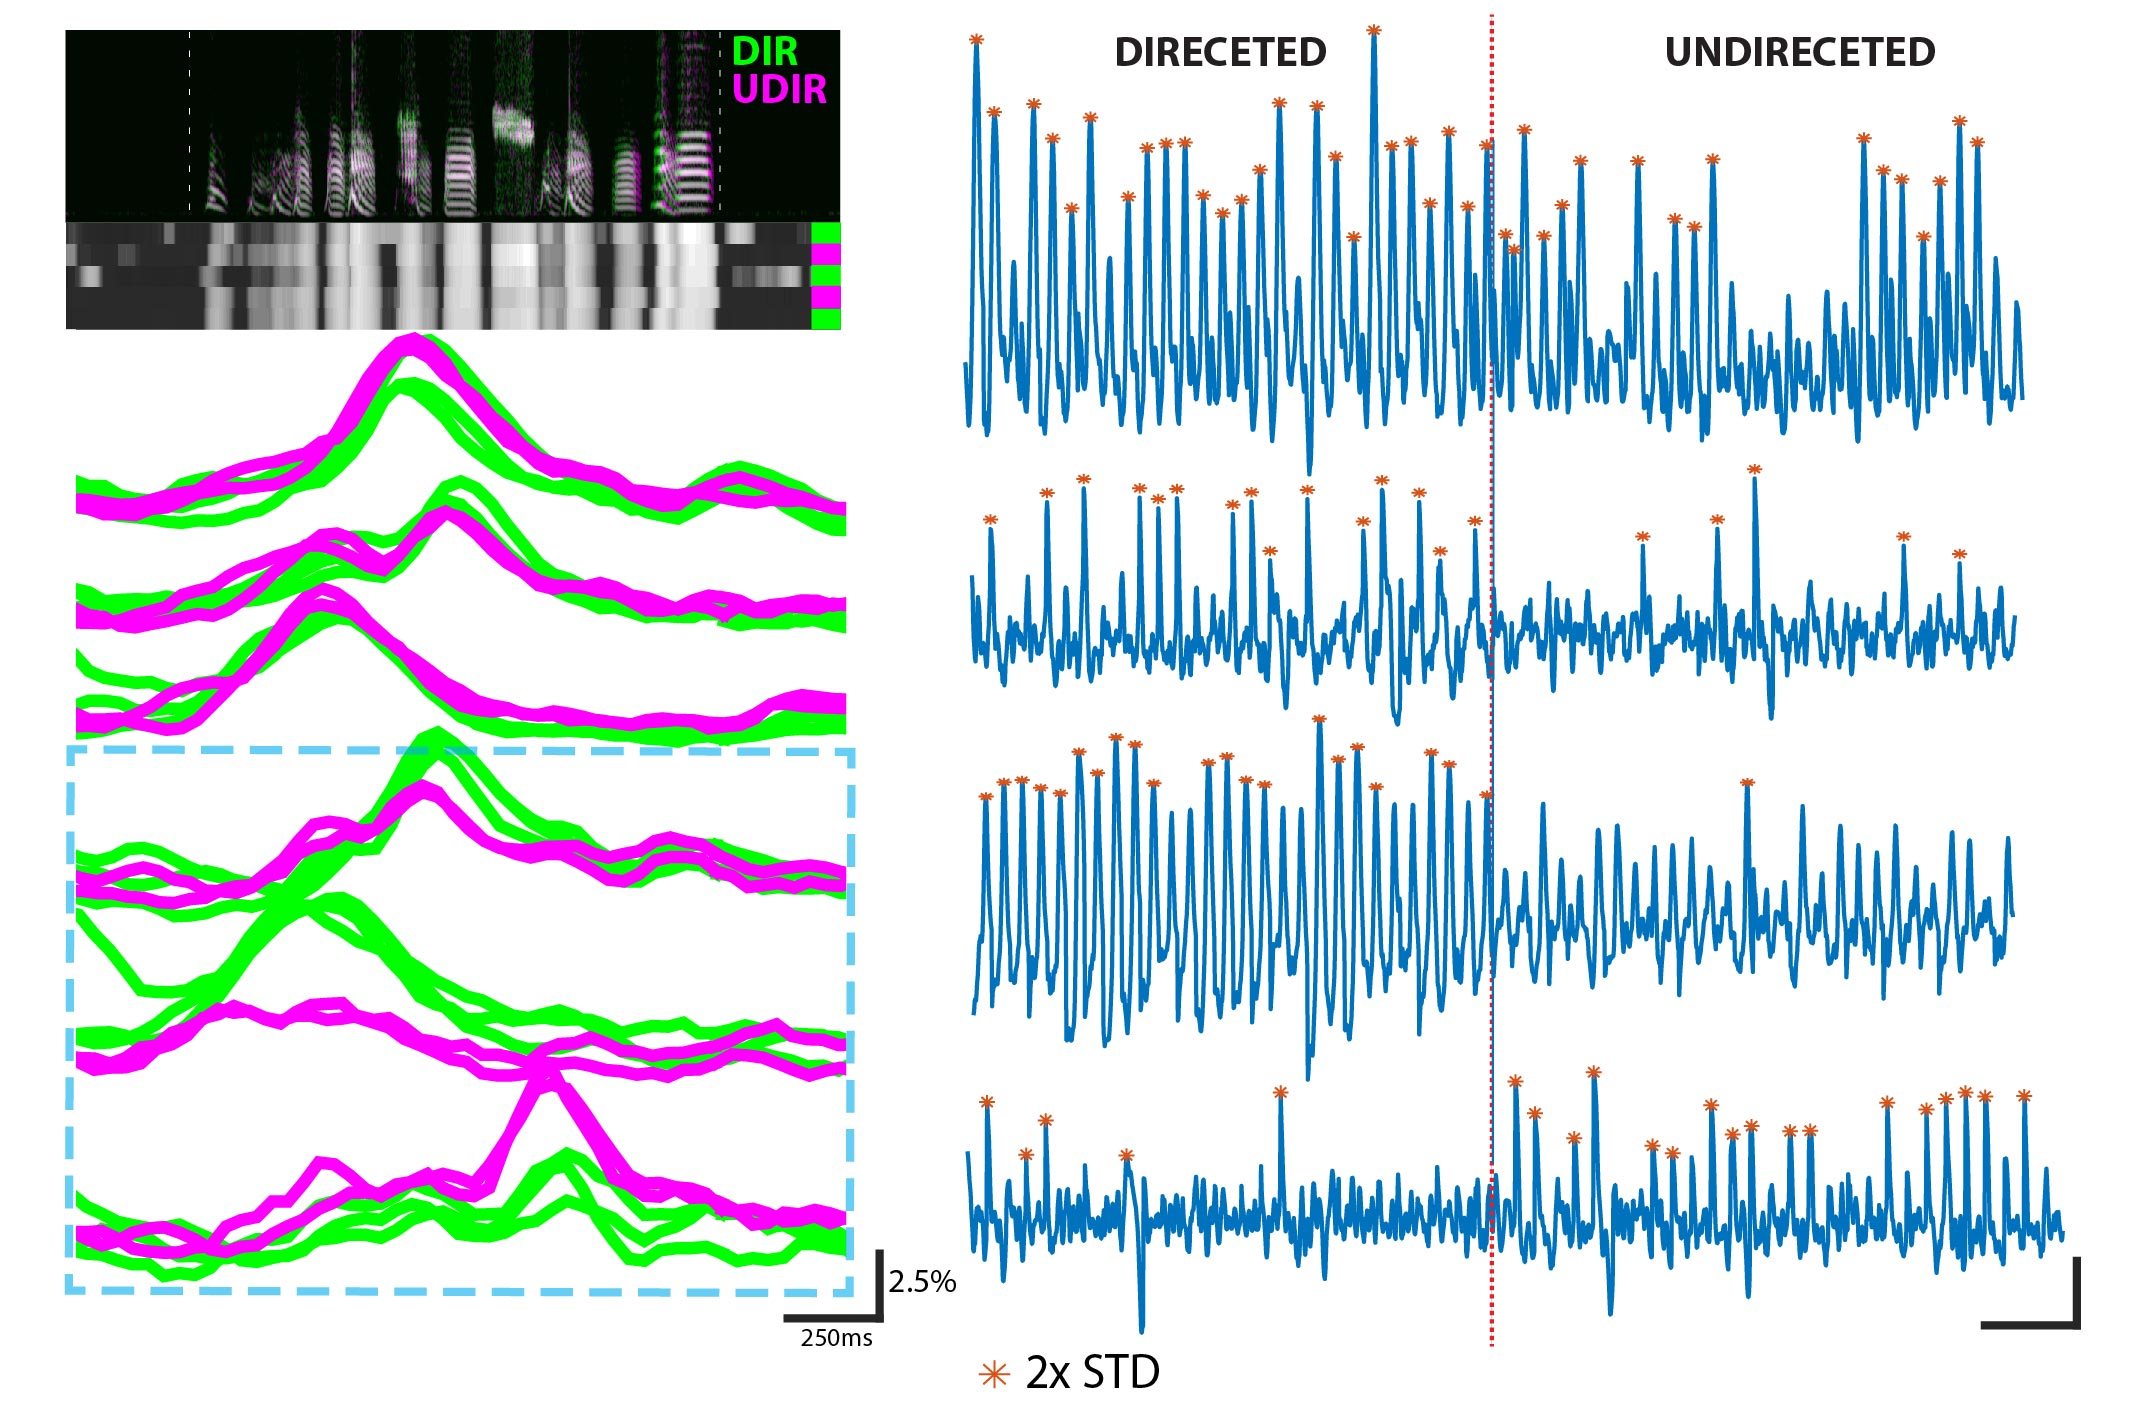
\includegraphics[width=11cm]{figure5.jpg}
    \centering
\medskip
\caption[Context related changes in HVC projection neurons ]{\footnotesize  \textbf{Context related changes in HVC projection neurons} Head-fixing animals may preclude the study of differences in motor coding that relate to the behavioral context of the animal. We see some evidence that motor codes that underlie song that is 'directed' to a female may differ from when song is produced in isolation.  \textit{Left,} Several ROIs aligned to song, from interleaved trials of directed and undirected song. Blue dotted-line inset highlights several ROIs the show some differences related to behavioral context. (Green = Directed, Magenta = undirected) \textit{Right,} fluorescent time series data from several ROIS, concatenated from many songs in each context. Differences in peak participation frequency in each context suggest that variabilities in coding may exist as a function of behavioral context.}

\label{fig:Sampling}
\end{figure}

 \begin{figure}[!htb]
 %\begin{minipage}[t]{0.49\linewidth}\centering
    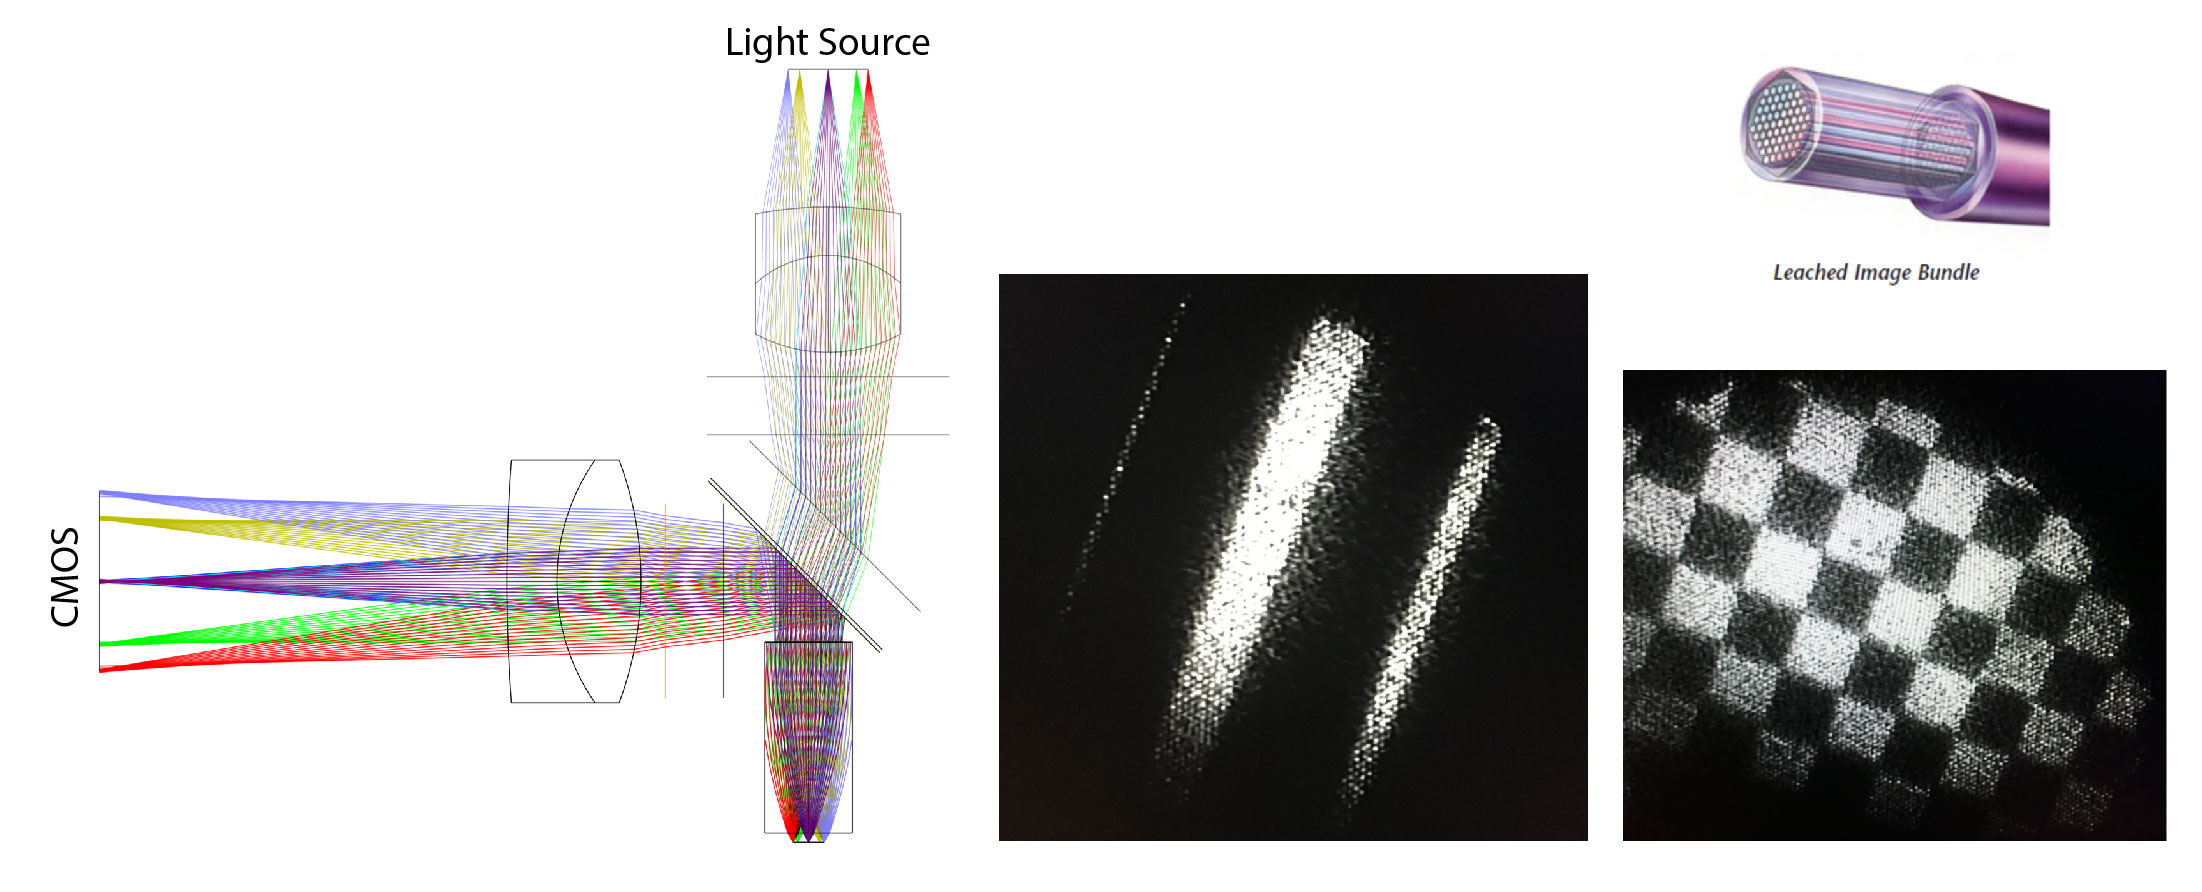
\includegraphics[width=11cm]{figure4.jpg}
    \centering
\medskip
\caption[Structured Illumination Integration]{\footnotesize  \textbf{Structured Illumination Integration} The integration of structured illumination into miniature microscopes would improve z-axis resolution, and could allow for arbitrary or patterned stimulation- creating all-optical interrogation, at the single cell level, in a freely behaving animal. \textit{Left,} Light-path for SIM integration. \textit{Right}, DMD patterns on the coherent fiber.}

\label{fig:Sampling}
\end{figure}
  
Compared to these laser scanning techniques, single photon imaging has relatively poor depth of field, z-axis sectioning, and tissue penetration. These issues can potentially be addressed using optical and computational techniques that improve signal quality by rejecting unwanted noise. The most promising of these techniques is Structured Illumination Microscopy (SIM). The increase in resolution from SIM is obtained by providing non-uniform excitation light patterns that feature sinusoidal intensity variations in one or more dimensions coupled with powerful image reconstruction techniques. This allows the rejection of out of focus light from outside of the image plane, at the expense of decreasing the effective frame-rate due to the computational step. Using micro LEDs and/or DMD coupled laser light deliver through coherent fiber bundles, SIM can be delivered through a custom designed miniature microscope. In preliminary experiments, a Digital Micro-mirror Device (Texas Instruments LightCrafter) is used to create three grid patterns that are shifted by a third of the period. After acquiring the three images, the sectioned image is computed and background fluorescence is rejected.  Extensions to this strategy could afford new ways to control neurons in freely behaving animals, using patterned illumination for optical control of spatially segregated neurons, and potentially could afford 3D volumetric imaging (Szabo et al. 2014). (Ventalon et al. 2015). Proof-of-concept work is currently occurring in an on-going collaboration with Bernardo Sabatini's lab in Harvard Medical School. Figure 6$\cdot$4 A fast cycle of ZEMAX optical path modeling and re-printing of the microscope housing has facilitated this collaborative engineering project, and has already demonstrated improvements in the rejection of out-of-plane fluorescence.





\section{ROI based, near-Real-Time Brain Machine Interface (BMI) experiments }


Motivated by the observation that the stability of song memory is rooted in the stability of network patterns that persist in spite of drifting individual neuron dynamics, we hope to explain the persistence of the song motor pattern in spite of unstable projection neurons. It is experimentally possible to directly test the hypothesis that changes in the firing patterns of single neurons in pre-motor cortex is beneficial to the motor program. I propose to explicitly test if the activity of these cells is shaped by the recent history of time-correlated reward or punishment signals, by using real-time Brain Machine Interfacing (BMI) experiments 
 
What is the utility of drifting motor commands in the production of a stable motor behavior? Previous studies using extracellular and intracellular recordings indicate that during vocal production,  HVC$_{X}$ and HVC$_{RA}$ neurons are insensitive to feedback perturbations, suggesting that performance evaluation does not occur in these cells during song. However, spine imaging studies have found that deafening shrinks and destabilizes dendritic spines on HVC$_{X}$ neurons within 12-48 hr and that these changes precede and predict the severity of song degradation. 


These results suggest that at least HVC$_{X}$ cells are sensitive to auditory feedback on the same timescale that we have observed drifting firing patterns. The descending projections of HVC$_{X}$ (and possibly HVC$_{AV}$) possibly  relay an efference copy of the motor control sequences that could be evaluated alongside song performance in the basal ganglia. In this case, we might expect some mechanism would exist at the interface of auditory and motor generation systems to consolidate and reconcile this evaluation. Perhaps  HVC serves as a structure where auditory feedback is ultimately integrated by constant fine-tuning of song motor commands. Individual cells slightly adapt their firing times to regulate the behavioral output of song after the accumulation and evaluation of performance errors, forming the mechanistic basis of memory maintenance and and motor stability. 


This could be tested using a variant of CAF where the auditory feedback is made contingent on the activity of single HVC, LMAN, or Area X neuron (Figure 6$\cdot$5). The aim would be to steer plasticity in cells that are already under observation. In this paradigm the bird can only escape aversive white noise playback by modulating the firing rate of either a single isolated unit, or group of units (Koralek et al. 2012) Potentially, this drift will be modulated by performance errors delivered through conditional auditory feedback and consolidated over periods of sleep.  This drift could be blocked or reduced by selective blockage of the output structures of the basal ganglia.
				
This use of region of interest (ROI) based feedback could be contingent on one or several neurons, and could be contrasted by feedback contingent on specific times in song in order to tease apart the individual contributions of individual cell types in HVC- although this strategy could be deployed across the song system. It would be critical to characterize the response of different cell types within a day, as well as the responses across days, to this feedback contingency in order to tease apart the cell-type specific mechanisms of motor adaptation. It would be equally interesting to monitor spontaneous activity during sleep, to observe what offline dynamics may be occurring that may predict changes or reinforce stable cells.

 
 \begin{figure}[!htb]
 %\begin{minipage}[t]{0.49\linewidth}\centering
    \includegraphics[width=11cm]{figure1.png}
    \centering
\medskip
\caption[BMI experimental outline]{\footnotesize  \textbf{BMI experimental outline} \textbf{a}, \textit{Left,} To perform experiments that can identify neural activity patterns in real time, the video stream is constantly processed to extract fluorescence information in pixels within predefined regions of interest. Rules (such as the ratio of activity in two ensembles) are applied to this near-real-time ROI analysis to trigger external events through a programmable digital output, such as white noise contingent on the pattern of activity recorded through the head-mounted microscope. In this mode, the camera provides a near-real-time brain machine interface allowing songbirds to control sounds directly through the measured calcium signals in the brain. Other BMI possibilities include closed-loop stimulation experiments that seek to electrically or optically disrupt patterns of activity in real-time.}
\label{fig:Sampling}
\end{figure}
 
 
 
 \section{The role of sleep}
The role of sleep, as it relates to motor systems, is not well-known. Chapter 5 describes changes in neural patterns that discretely occur overnight, raising the possibility that new patterns of activity 'invented' over intervals of sleep provide important raw material for song learning and maintenance. Francis Crick proposed that noisy reactivation of neural circuits in sleep weakens the strongest pathways in the brain, promoting adaptive plasticity. This leads us to ask: Do new strategies of motor exploration occur over periods of sleep, seeking the source of variability and motor-sequence exploration both during periods of song and during 'offline' periods? It is possible that spontaneous activity patterns in sleep allow injection of randomness that allows for fine grade motor exploration through subtle changes in synaptic weights. This may be visualized in large scale changes seen across days, which may be guided or biased within a day by small populations of auditory and/or context sensitive neurons. 
 
Sleep is widely believed to be important for learning and memory, particularly in the process of consolidation, a process that transforms short-term memories into more stable longer-term memory representations (Kuriyama, Stickgold, and Walker 2004)  (Walker and Stickgold 2004)  (Stickgold and Walker 2004)  (Diekelmann and Born 2010). Many theoretical models propose that consolidation would benefit from sleep, suggesting that sleep prevents the possible interference of daily activities on memory consolidation (Diekelmann and Born 2010). However, experimental evidence explicitly demonstrates that this process is sparse. 

Learning new tasks is often associated with stabilization of ensemble activity patterns across days as well as increased task-related neuronal activity. The emerging picture is that neuronal representations are explored by behavioral relevance during the day, but that long-term integration of beneficial changes occurs during offline periods. This 'consolidation' may  transform short-term optimal network configurations, that may be inherently fragile and plastic, into more stable and long-term stored memory representations without the interference of online processes (Ferry and McGaugh 2000; Izquierdo and McGaugh 2000)  (Eisenberg and Dudai 2004) (Diekelmann and Born 2010) (Diekelmann and Born 2010)

 \begin{figure}[!htb]
 %\begin{minipage}[t]{0.49\linewidth}\centering
    \includegraphics[width=11cm]{figure6.png}
    \centering
\medskip
\caption[Spontaneous activity during sleep]{\footnotesize  \textbf{Spontaneous activity during sleep} \textit{Top}, activity during sleep, contrasted with \textit{Bottom}, song related neural activity. }
\label{fig:Sampling}
\end{figure}
 
During sensorimotor learning of song in juvenile zebra finches, improvements in structure from the previous day deteriorated over a night of sleep, but through the following day improved and surpassed the previous day's quality. Interestingly, juveniles that showed the most 'backsliding' as a result of sleep, achieved the best tutor song imitation as adults (Der�gnaucourt et al. 2005). In addition, spontaneous activity during sleep in juvenile male zebra finches was correlated to the quality of tutor song imitation (Gobes, Zandbergen, and Bolhuis 2010). In the adult, spontaneous neuronal activation during sleep in several parts of the song system appear to resemble motor activation patterns that drive song (Dave and Margoliash 2000). Moreover, there is evidence that noisy or partially incomplete  spontaneous sequence reactivations of the motor plan occur during sleep in the motor region RA(Shank and Margoliash 2009). Taken as a whole, there is strong evidence that sleep plays a role in memory formation in songbirds and that this may be critical for the learning and maintenance of song. (Gobes, Zandbergen, and Bolhuis 2010; Gobes and Bolhuis 2008)

Future experiments are needed to robustly answer how sleep is involved in motor stability and planning. I believe that the zebra finch will presents itself as an ideal model system for addressing these questions; the extreme precision and long-term stability of song structure offers a unique opportunity to observe how motor memories are maintained at the network level- and how these networks are shaped by different states, like sleep. Using cell-type specific genetically encoded calcium indicators and custom miniature head-mounted microscopes, neural populations can be observed over weeks and months. Combining the use of near real-time behavioral and neurally guided feedback mentioned in the previous section, along with round-the-clock monitoring of neural activity will help elucidate the learning roles of individual cells the lead to stable memories.

 





\cleardoublepage

%\appendix
\begin{appendices}
\chapter{Proof of xyz}
\label{appendix}
\thispagestyle{myheadings}

This is the appendix.
\end{appendices}
%==========================================================================%
% Bibliography
\newpage
\singlespace
\bibliographystyle{apalike}

% each subdirectory can have its own BiBTeX file
\bibliography{thesis}
\cleardoublepage

%==========================================================================%
% Curriculum Vitae
\addcontentsline{toc}{chapter}{Curriculum Vitae}

\thispagestyle{empty}

\begin{center}
{\LARGE {\bf CURRICULUM VITAE}}\\
\vspace{0.5in}
{\large {\bf Joe Graduate}}
\end{center}

Basically, this needs to be worked out by each individual, however the same format, margins, typeface, and type size must be used as in the rest of the dissertation. 
 

%==========================================================================%
\end{document}
